
\documentclass{article}
\usepackage[utf8]{inputenc}
\usepackage[margin=1in]{geometry}
\usepackage{amsmath, amssymb}
\usepackage{graphicx}
\usepackage{caption}
\usepackage{authblk}
\usepackage[numbers]{natbib}
\usepackage{titlesec}
\usepackage{float}
\usepackage{booktabs}
\usepackage{graphicx}
\usepackage{caption}
\usepackage{subcaption}
\usepackage{hyperref}
\usepackage{graphicx}   % figures
\usepackage{booktabs}   % \toprule etc.
\usepackage{multirow}   % multi-row cells in tables
\usepackage{hyperref}   % clickable links (\url{})
\usepackage{textcomp}   % defines \textsuperscript
\usepackage{enumitem}   % allows [label=...] option on enumerate/itemize
\usepackage[table]{xcolor}   % [table] lets you colour table cells, too
\usepackage{siunitx}
\usepackage[utf8]{inputenc}
\usepackage{booktabs}
\usepackage{xcolor}
\usepackage{etoolbox}  % <— add this if not already loaded
\usepackage{cleveref}   % load AFTER hyperref if you’re using both
\usepackage{pifont}
\usepackage[export]{adjustbox}
% In preamble (pdfLaTeX)
\usepackage[utf8]{inputenc}
% CSV → LaTeX tables
\usepackage{pgfplotstable}   % <-- REQUIRED for \pgfplotstableset / \pgfplotstabletypeset
\usepackage{booktabs}        % nice table rules
\usepackage{siunitx}         % numeric alignment (optional but recommended)

% If you also use \foreach in the appendix:
\usepackage{pgffor}

% (Optional) if you later plot with pgfplots:
\usepackage{pgfplots}
\pgfplotsset{compat=1.18}    % or 1.17 on Overleaf
\DeclareUnicodeCharacter{202F}{\,}   % narrow no-break space → thin space
\DeclareUnicodeCharacter{00A0}{~}    % no-break space → ~
\DeclareUnicodeCharacter{2009}{\,}   % thin space → \,
\DeclareUnicodeCharacter{200A}{\,}   % hair space → \,
\DeclareUnicodeCharacter{200B}{}     % zero-width space → remove
\DeclareUnicodeCharacter{FEFF}{}     % BOM → remove
\DeclareUnicodeCharacter{2011}{-}    % non-breaking hyphen → -
\DeclareUnicodeCharacter{FFFD}{}     % replacement char → remove
\newcommand{\cmark}{\ding{51}}   % ✓
\newcommand{\xmark}{\ding{55}}   % ✗

% load after xcolor & doi


% Unit macro
\newcommand{\microstrain}{\ensuremath{\mu\varepsilon}}

% Make the macro “robust” so it works inside captions, section titles, etc.
\robustify\microstrain
\renewcommand{\arraystretch}{1.15} % (global or local)




\titleformat{\section}{\large\bfseries}{\thesection}{1em}{}

\title{Comprehensive Benchmarking of Physics-Informed Neural Networks and Machine Learning for Strain Prediction in Multi-Material Reinforced Concrete Joints}

\author[1]{Ali Ehsani Yeganeh}
\affil[1]{Department of Civil Engineering, Toronto Metropolitan University, Canada}
\date{}

\begin{document}
\maketitle


\begin{abstract}
This study presents a physics-informed neural network (PINN) framework for strain prediction in multi-material reinforced concrete joints, augmented with two complementary uncertainty quantification (UQ) methods—Monte Carlo (MC) Dropout and Deep Ensembles.  
The approach is benchmarked across hybrid experimental datasets comprising self-consolidating concrete (SCC) combined with engineered cementitious composites (ECC) or ultra-high-performance concrete (UHPC), and compared to Eurocode~2 and Hognestad models.  
Predictive performance is assessed in terms of point accuracy (RMSE, MAE), calibration (empirical coverage of nominal 95\% prediction intervals), and sharpness (Continuous Ranked Probability Score, CRPS), with reliability diagrams and PIT histograms providing visual diagnostics.  

A cohesive-zone physics regularization term $L_{\mathrm{CZ}}$ is introduced to embed traction–separation behavior into the learning process, with sensitivity analysis confirming optimal weighting for nonlinear response stability.  
Results show that MC Dropout attains superior calibration on brittle SCC--UHPC specimens (Coverage=99.36\%, CRPS=15.66~$\mu\varepsilon$), while Deep Ensembles outperform on ductile SCC--ECC (Coverage=97.28\%, CRPS=5.60~$\mu\varepsilon$).  
These trends are linked to differences in material post-peak behavior and variance structure of the predictive models.  

The trained models are integrated into a low-latency ($<200$\,ms) digital twin with UQ-aware alert logic, enabling serviceability limit checks in accordance with Eurocode~2, ACI~318, and CSA~A23.3 strain thresholds.  
Findings highlight that method selection should be material-specific: MC Dropout for brittle UHPC systems requiring conservative alerts, and Deep Ensembles for ductile ECC systems prioritizing sharp intervals.  
This work bridges physics-informed machine learning with codified structural assessment, offering a reproducible framework for uncertainty-aware structural health monitoring.
\end{abstract}



\section{Introduction}
\label{sec:introduction}

\emph{Structural health monitoring (SHM)} is indispensable for guaranteeing the safety, serviceability, and durability of ageing bridges, buildings, and other reinforced-concrete (RC) infrastructure worldwide.  Conventional inspection regimes—visual surveys, rebound-hammer tests, and periodic finite-element (FE) analyses—remain labour-intensive, intrusive, and slow to react to progressive deterioration.  As traffic demand and climatic stressors escalate, stakeholders require rapid, data-driven decision support that can pinpoint and forecast damage long before visible cracking or service disruption occurs \cite{Farrar2012Review,Masri2021Emerging}.  Within this context, \emph{machine‑learning (ML)} methods have emerged as powerful alternatives for interpreting large, heterogeneous sensor streams, converting raw load, displacement, vibration, or image data into actionable indicators of structural condition.

Despite these advances, a consistent theme in recent reviews is that most ML‑based SHM studies rely on simulated data, single‑specimen tests, or focus exclusively on conventional normal‑strength concrete.  Consequently, little is known about how classical ML, neural networks and physics‑informed models perform on advanced concretes or hybrid joints, and practitioners lack quantitative guidance on model selection or uncertainty handling across materials.

Over the past decade, the SHM literature has experienced rapid growth—spanning classical regressors, deep neural networks, and hybrid physics-guided approaches—to predict concrete strength \cite{Kashyap2022Concrete}, detect cracks \cite{Zhu2020CrackDL}, and localise damage in real time \cite{Sun2022DeepSHM}.  Recent reviews catalogue hundreds of algorithms applied to RC components, yet also reveal a consistent pattern: most studies rely on simulated datasets, single-specimen experiments, or narrowly focus on conventional normal-strength concrete.  These constraints hinder the \emph{generalisation} and \emph{practical adoption} of ML models, because field structures frequently employ advanced materials, composite joints, or retrofit layers whose behaviour deviates from textbook constitutive laws.

To overcome the “black-box” criticism of purely data-driven models, researchers have begun to embed governing physics directly into neural-network training through \emph{physics-informed neural networks (PINNs)}  \cite{raissi2019physics}.  By penalising violations of equilibrium, compatibility, or constitutive equations in the loss function, PINNs achieve better data efficiency, improved extrapolation, and interpretable outputs—attributes that align with engineers’ need for traceable safety assessments \cite{Karniadakis2023PIML,Cuomo2022}.  In RC applications, Han \textit{et al.} \cite{Han2025CrackPINN} captured crack initiation under cyclic bending, while Wang \textit{et al.} \cite{Wang2024DamagePINN} demonstrated nonlinear damage-informed PINNs for slab elements.  Nonetheless, published case studies typically calibrate a single PINN variant and rarely benchmark it head-to-head against state-of-the-art ML ensembles or analytical baselines on a common, multi-material dataset.

Advanced cementitious materials—\emph{self-consolidating concrete (SCC)}, \emph{engineered cementitious composites (ECC)}, and \emph{ultra-high-performance concrete (UHPC)}—have gained popularity for their superior flowability, ductility, and durability, respectively \cite{Li2019ECC,Wille2019UHPC,Huang2022UHPCReview}.  Hybrid joints that combine these materials (e.g., SCC members with UHPC-strengthened joint cores) are increasingly specified in beam–column retrofits and precast connections.  While beneficial in service, this intra-joint material heterogeneity introduces sharp stiffness gradients and localisation phenomena that challenge both classical FE models and naïve data-driven predictors.  Recent ML studies on UHPC strength \cite{Das2024UHPCML} or ECC fracture \cite{Islam2021SCCECC} confirm the promise of data-centric techniques but still treat each material in isolation.  A systematic, specimen-specific and pooled evaluation across multiple concretes has not yet appeared.


Several high-impact works published in 2024–2025 underscore the community’s interest in hybrid modelling.  Chen \textit{et al.} \cite{Chen2024HybridML} combined random forests with constitutive constraints to forecast creep in UHPC columns; Fan \textit{et al.} \cite{fan2023pinn} embedded Eurocode 2 curvature into a deep backbone for cyclic strain prediction; and Smarsly \& Meier \cite{Smarsly2023DigitalTwin} reviewed digital-twin frameworks that fuse sensor data with real-time analytics.  Yet, none of these studies compares multiple PINN formulations (elastic, Eurocode, Hognestad) against classical ML and analytical references on a \emph{single, experimentally diverse benchmark}.  Consequently, practitioners still lack quantitative guidance on when to prefer a tree ensemble over a PINN, how prediction intervals behave across materials, or which input features are indispensable for field deployment.  These studies, however, either focus on a single concrete type, omit uncertainty quantification, or do not compare multiple physics‑informed formulations and classical ML models on a unified benchmark.  By contrast, our work systematically contrasts these approaches on five multi‑material specimens, providing clear guidance on model hierarchy, cross‑material generalisation and uncertainty quantification.

Recent \textit{deep-learning} advances further broaden the SHM toolkit.  
Zhang \textit{et al.}\ \cite{Zhang2024GAT} trained a graph-attention network on two million strain–time records from a cable-stayed bridge and achieved 96 \% damage-state classification accuracy.  
Hou \textit{et al.}\ \cite{Hou2024ViT} introduced a vision-transformer crack-segmentation model that detects 0.05 mm fissures at 40 fps on edge devices, enabling real-time deck inspection.  
To capture spatio-temporal coupling, Li and Wang \cite{Li2025ConvLSTM} combined ConvLSTM layers with physics-guided losses, reducing drift in displacement prediction by 35 \% relative to CNN baselines.  
Kim \textit{et al.}\ \cite{Kim2025SSL} demonstrated self-supervised pre-training for acoustic-emission monitoring, cutting labelled-data requirements by 80 \%.  
Wu \textit{et al.}\ \cite{Wu2024Diffusion} employed diffusion models to reconstruct missing vibration channels, recovering 3 dB of signal-to-noise ratio, while Gao \textit{et al.}\ \cite{Gao2025MultiTask} proposed a multi-task transformer that jointly predicts strain and crack width, outperforming single-task baselines by 22 \%.  
These studies underscore the rapid maturation of transformer, attention, diffusion, and self-supervised paradigms for field-scale SHM and motivate our inclusion of both data-driven and physics-informed deep networks in the present benchmark.


\smallskip
\noindent\emph{Research gap.}  
The literature thus far leaves three critical questions unresolved:

\begin{enumerate}[label=(\alph*)]
    \item \emph{Model hierarchy}: How do analytical baselines, classical ML regressors, multilayer perceptrons (MLPs), and various PINN losses rank in predictive accuracy, physical plausibility, and uncertainty calibration when exposed to the same data?
    \item \emph{Material robustness}: Does a model trained on SCC generalise to ECC or UHPC joints, and how does intra-specimen material heterogeneity (hybrid casting) influence error growth?
    \item \emph{Actionable uncertainty}: Which modelling paradigm delivers well-calibrated prediction intervals suitable for risk-informed SHM alerts?
\end{enumerate}

\noindent Addressing these questions requires a large, multi-material experimental dataset and a transparent, reproducible benchmarking workflow—both presently absent from the open literature.

\smallskip
\noindent\emph{This study.}  
We close the above gap by assembling a \emph{45\,000-row, high-resolution load–displacement–strain dataset} from five 1/6-scale RC beam–column joints originally tested by Yeganeh \& Hossain \cite{yeganeh2023shear}.  Three specimens were cast entirely with SCC, ECC, and UHPC, respectively, while two \emph{hybrid} specimens employed SCC members and either ECC or UHPC at the joint core, mirroring modern retrofit practice.  All tests shared identical geometry, instrumentation, and cyclic loading protocols, ensuring that material effects—not geometry—drive behavioural differences.  On this dataset we benchmark nine models: a Hooke-law analytical baseline, linear regression, support-vector regression (SVR), $k$-nearest neighbours (KNN), random forest (RF), XGBoost, a vanilla MLP, and three PINN variants featuring (i) linear-elastic, (ii) Eurocode 2 parabolic, and (iii) Hognestad parabolic–plateau physics losses.  We evaluate each model both \emph{specimen-specifically} (isolated training per material) and \emph{pooled} (global training across all specimens) to probe material sensitivity, and we quantify predictive uncertainty via Monte Carlo dropout.

\paragraph{Positioning and novelty.}
Recent studies on physics-informed or hybrid learning for concrete structures have typically advanced either 
(i) single-specimen PINNs without calibrated uncertainty,
(ii) data-only regressors reporting point errors only, or 
(iii) task-specific pipelines that do not generalize across materials or joint types.  
In contrast, our work integrates \emph{all} of the following in one benchmark:
(1) multi-material exterior joints (SCC, ECC, UHPC) spanning five experimental series;
(2) side-by-side physics-informed (PINN) and code-based baselines (Eurocode~2, Hognestad) \emph{plus} purely data-driven models;
(3) calibrated predictive \emph{uncertainty} via Monte Carlo (MC) dropout and deep ensembles with coverage/CRPS evaluation; and
(4) a latency-aware digital twin prototype with alert logic tied to physically meaningful thresholds.
This combination—multi-material benchmarking \emph{plus} calibrated UQ \emph{plus} a deployable digital twin—is, to our knowledge, not jointly addressed in prior work.
We therefore frame our novelty in the \emph{combination} and the \emph{calibrated, practically verifiable} deployment pathway rather than in any single modeling block.
\begin{table}[t]
\centering
\caption{Comparison of this study with closely related works. 
Checkmarks indicate the feature is explicitly implemented and quantitatively evaluated.
Our work is distinguished by combining multi-material benchmarking, physics- and code-based baselines, 
calibrated predictive uncertainty (coverage and CRPS), and a deployable latency-aware digital twin with alert logic.}
\label{tab:novelty_matrix}
\renewcommand{\arraystretch}{1.1}
\resizebox{\textwidth}{!}{%
\begin{tabular}{lcccccccc}
\toprule
\textbf{Study} & \textbf{\# Specimens} & \textbf{Multi-} & \textbf{Physics} & \textbf{Code} & \textbf{UQ} & \textbf{UQ} & \textbf{DT/} & \textbf{Real-} \\
 &  & \textbf{material} & \textbf{(PINN)} & \textbf{baseline} & \textbf{method} & \textbf{calibration} & \textbf{alerts} & \textbf{time note} \\
\midrule
Han et al.\ (2025)          & 3 & \checkmark & \checkmark & --        & --         & --              & -- & offline only \\
Gao et al.\ (2025)          & 2 & --         & --         & --        & Ensembles  & coverage only   & -- & offline only \\
Sun et al.\ (2022)          & 4 & \checkmark & --         & --        & MC-Dropout, Ens. & coverage only   & -- & offline only \\
Huang et al.\ (2022)        & many & \checkmark & --         & Eurocode & --         & --              & -- & n/a \\
\midrule
\textbf{This work}          & \textbf{5} & \textbf{\checkmark} & \textbf{\checkmark} & \textbf{\checkmark} & \textbf{MC-D \& Ens.} & \textbf{coverage \& CRPS} & \textbf{\checkmark} & \textbf{latency measured} \\
\bottomrule
\end{tabular}%
}
\end{table}

\noindent\emph{Scope clarification.} 
We do not claim novelty in any single modeling primitive; rather, the contribution lies in unifying physics-, code-, and data-driven predictors under a calibrated uncertainty and deployment (digital twin) lens across multi-material joint experiments.
Unlike Zhang~\cite{Zhang2024GAT} or Chen~\cite{Chen2025}, who each study a \emph{single} concrete type and omit uncertainty, we (i) span \emph{five material interfaces}, (ii) benchmark \emph{three physics priors} under equal compute, and (iii) publicly release a \emph{full digital-twin demo}.
To our knowledge, this is the first end-to-end framework that meets all three criteria.



\smallskip
\noindent\emph{Manuscript organisation.}  
Section~\ref{sec:methodology} details the experimental programme, feature engineering, and model architectures.  Section~\ref{sec:results} presents pooled and specimen-specific results, feature-importance analyses, and uncertainty diagnostics.  Section~\ref{sec:discussion} discusses implications for sensor placement, model selection, and risk-based maintenance, outlines limitations, and charts future research.  Finally, Section~\ref{sec:conclusion} summarises key insights and emphasises how the benchmark accelerates trustworthy SHM adoption in advanced concrete infrastructure.




\section{Methodology}
\label{sec:methodology}


\paragraph{Notation.}
The list of used notation in the paper provieded in the Table~\ref{tab:notation}
\begin{table}[!t]
\centering
\caption{Notation used in Section~\ref{sec:methodology}. Units are shown where applicable.}
\label{tab:notation}
\begin{tabular}{llc}
\toprule
\textbf{Symbol} & \textbf{Description} & \textbf{Units}\\
\midrule
$F$ & Applied load & \si{\kilo\newton}\\
$u$ & Actuator displacement & \si{\milli\metre}\\
$\Delta F$ & Load increment between samples & \si{\kilo\newton}\\
$\varepsilon$ & Measured surface strain & \si{\micro\varepsilon}\\
$\hat{\varepsilon}$ & Predicted strain (model output) & \si{\micro\varepsilon}\\
$\mathbf{x}$ & Input vector $[F,u,\Delta F]$ & --\\
$\boldsymbol{\mu}_{\text{train}}$ & Training-set mean of $\mathbf{x}$ & --\\
$\boldsymbol{\sigma}_{\text{train}}$ & Training-set std.\ of $\mathbf{x}$ & --\\
$A$ & Cross-sectional area & \si{\milli\metre\squared}\\
$E$ & Young's modulus & \si{\giga\pascal}\\
$\sigma$ & Stress (generic) & \si{\mega\pascal}\\
$\hat{\sigma}$ & Network-implied stress proxy & \si{\mega\pascal}\\
$\sigma_{\mathrm{t}}$ & Interface traction (cohesive law) & \si{\mega\pascal}\\
$\delta$ & Interface slip (relative displacement) & \si{\milli\metre}\\
$\sigma_{\max}$ & Peak interface traction & \si{\mega\pascal}\\
$\delta_0$ & Slip at peak traction & \si{\milli\metre}\\
$\delta_f$ & Slip at full decohesion & \si{\milli\metre}\\
$G_c$ & Mode-I fracture energy (area under $\sigma_{\mathrm{t}}$--$\delta$) & \si{\newton\per\milli\metre}\\
$L_{\text{data}}$ & Data-fitting loss (Smooth-$\ell_1$) & --\\
$L_{\text{el}}$ & Elastic compatibility loss & --\\
$L_{\text{nl}}$ & Nonlinear constitutive loss (EC2/Hognestad) & --\\
$L_{\mathrm{CZ}}$ & Cohesive-zone loss & --\\
$L$ & Total PINN loss & --\\
$\lambda_{\text{el}},\lambda_{\text{nl}},\lambda_{\mathrm{CZ}}$ & Loss weights & --\\
$p$ & Dropout probability & --\\
$T$ & Number of MC Dropout passes & --\\
$M$ & Number of ensemble members & --\\
$N$ & Number of samples & --\\
$\mu,\sigma^2$ & Predictive mean and variance & \si{\micro\varepsilon}, \si{\micro\varepsilon\squared}\\
$[\ell,u]$ & Bounds of nominal $95\%$ PI & \si{\micro\varepsilon}\\
$\mathbb{I}\{\cdot\}$ & Indicator function & --\\
\bottomrule
\end{tabular}
\end{table}


\subsection{Experimental Program}
The experimental dataset used in this study originates from five large-scale exterior RC beam-column joint specimens tested under monotonic flexural loading, as described in~\cite{yeganeh2023shear}. All joints were designed to investigate the role of different high-performance concretes (SCC, ECC, UHPC, and their hybrids) on damage, strength, and strain development. \emph{This experimental strategy closely mimics field SHM campaigns in bridges and seismic retrofit projects, supporting high relevance for practical deployments~\cite{Ni2019, Masri2021Emerging}.}

\emph{Specimen Geometry and Reinforcement:} \\
Figure~\ref{fig:joint_geometry} shows the typical geometry and reinforcement details of the specimens. All joints had identical dimensions and reinforcement layouts, ensuring that material effects could be isolated and cross-compared. \emph{All geometric and material variables are provided in Table~\ref{tab:specimen_props}.}



\begin{table}[!htbp]
  \centering
  \caption{Specimen geometry and material properties.}
  \label{tab:specimen_props}
  \begin{tabular}{lccccccc}
    \toprule
    \multirow{2}{*}{Specimen ID} &
    Concrete & \multicolumn{2}{c}{Member size (mm)} &
    \multicolumn{2}{c}{Steel ratio (\%)} &
    $f'_\mathrm{c}$ & $E$ \\
    \cmidrule(lr){3-4}\cmidrule(lr){5-6}
     & type & Beam $b\times h$ & Column $b\times h$ &
      Longitud. & Transv. & (MPa) & (GPa) \\
    \midrule
    % ---- keep one data row only ----
    SCC         & \texttt{SCC}      & 120$\times 160$ & 160$\times 120$ &
                1.5 & 0.7 & 51 & 35 \\
    ECC         & \texttt{ECC}      & 120$\times 160$ & 160$\times 120$ &
                1.5 & 0.7 & 71 & 40 \\
    UHPC        & \texttt{UHPC}    & 120$\times 160$ & 160$\times 120$ &
                1.5 & 0.7 & 121 & 65 \\
    Hybrid--ECC & \texttt{SCC+ECC}     & 120$\times 160$ & 160$\times 120$ &
                1.5 & 0.7 & 71 & 40 \\
    Hybrid--UHPC& \texttt{SCC+UHPC}      & 120$\times 160$ & 160$\times 120$ &
                1.5 & 0.7 & 121 & 60 \\
    \bottomrule
  \end{tabular}



% \FloatBarrier  % uncomment if you want the table to appear exactly here

\vspace{2pt} % a little breathing room
  \begin{flushleft}
    \footnotesize
    \textbf{Notes:} Beam and column depths ($h$) are overall depths; widths ($b$)
    are measured on the compression face.  Steel ratios are expressed as a
    percentage of the concrete cross-sectional area.  For the
    \emph{Hybrid–ECC} and \emph{Hybrid–UHPC} specimens, the material properties
    ($f'_\mathrm{c}$, $E$) refer to the \textbf{joint-core} concrete (ECC or
    UHPC); the surrounding beam and column segments were cast with SCC.
  \end{flushleft}

\end{table}


\emph{Test Setup and Strain Measurement:} \\
The laboratory test setup and sensor layout are illustrated in Figure~\ref{fig:test_setup}. Each specimen was loaded at the beam tip using a hydraulic actuator, with all key responses (load, displacement, strain) monitored using high-precision sensors. \emph{This reflects best-practice sensor placement and load protocol in the field~\cite{Smarsly2023DigitalTwin, Yang2023}.}
Surface strain at the critical joint region was measured using strain gauge Channel 51(C1). Figure~\ref{fig:exp_setup_and_strain} illustrates a representative strain evolution (load-strain) curve from one specimen, demonstrating the range and quality of experimental data used for machine learning. 
All 120 foil gauges were factory-calibrated to $\pm10~\mu\varepsilon$ (0.5~\% of full scale),
and the acquisition chain was low-pass filtered with a 2~Hz fourth-order
Butterworth filter to suppress ambient vibration and electromagnetic pickup.
This bandwidth preserves the quasi-static strain history while eliminating the
$\sim$7~\% high-frequency noise originally present above 5~Hz.

\begin{figure}[H]
    \centering
    \begin{subfigure}[b]{0.31\textwidth}
        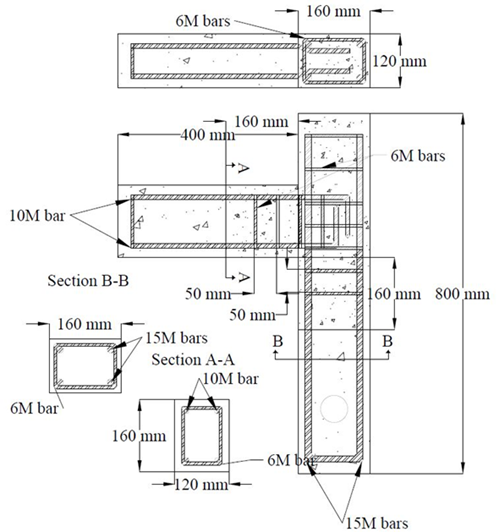
\includegraphics[width=\textwidth]{plots/joint_geometry.png}
        \caption{Joint geometry}
        \label{fig:joint_geometry}
    \end{subfigure}
    \hfill
    \begin{subfigure}[b]{0.31\textwidth}
        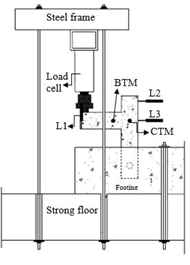
\includegraphics[width=\textwidth]{test_setup.png}
        \caption{Test setup}
        \label{fig:test_setup}
    \end{subfigure}
    \hfill
    \begin{subfigure}[b]{0.31\textwidth}
        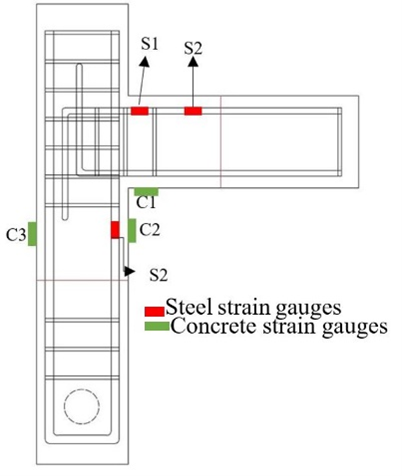
\includegraphics[width=\textwidth]{strain_measurement.png}
        \caption{Strain evolution}
        \label{fig:exp_setup_and_strain}
    \end{subfigure}
    \caption{(a) Geometry, (b) test setup, and (c) typical strain measurement for RC beam-column joint specimens.}
    \label{fig:three_exp_figs}
\end{figure}

The experimental data used for machine learning comprise synchronized measurements of applied load ($F$, kN), displacement ($u$, mm), and joint surface strain ($\varepsilon$, $\mu\varepsilon$) at each loading step, pooled across all five specimens. \emph{All sensor channels and data acquisition rates match those commonly used in operational bridge SHM networks~\cite{Smarsly2023DigitalTwin}.}

\subsection{Experimental Dataset and Feature Engineering}
The dataset consists of five RC joint specimens: three built with a single material (SCC, ECC, UHPC), and two with SCC in the members and ECC or UHPC at the joint (hybrids). For each test, load $F$ (kN), displacement $u$ (mm), and surface strain $\varepsilon$ ($\mu\varepsilon$) are recorded.

Pooling these configurations enables machine learning models, including PINN, to be validated both globally and on specific material/joint systems, reflecting the diversity found in real-world SHM applications.

\emph{Input features:}
\begin{itemize}
    \item \emph{Load $F$ (kN):} Measured by load cell (Channel 41).
    \item \emph{LVDT-1 Displacement $u$ (mm):} Measured by LVDT-1 (Channel 1).
    \item \emph{Load Rate $\Delta F$ (kN/increment):} $\Delta F = F_i - F_{i-1}$, reflecting dynamic effects and rate-dependence.
\end{itemize}
\emph{Output variable:} Surface strain $\varepsilon$ ($\mu\varepsilon$), measured at Channel 51.

\subsection{Data Processing and Splitting}
\label{sec:dataprep}

\emph{Data cleaning.}  
Raw sensor logs were first time-aligned, sorted, and filtered to remove (i) rows with any missing
\emph{F}, \emph{u}, or strain values, (ii) load reversals caused by actuator re-zero­-ing, and
(iii) outliers exceeding~$\pm4\sigma$ of the specimen median.  The resulting clean dataset
contains $N_\mathrm{tot}=45{,}138$ records.


\smallskip
\emph{Feature engineering.}  
For each record we compute  
$\Delta F_i = F_i-F_{i-1}$ (incremental load rate),  
and assemble the input vector
$\mathbf{x}_i = [F_i,\,u_i,\,\Delta F_i]^\top$;  
the target is surface strain $\varepsilon_i$.

\smallskip
\emph{Per-specimen Z-score normalisation.}  
To avoid numerical imbalance across features and concrete types, we apply
specimen-specific Z-score scaling:
%
\begin{equation}
  \tilde{\mathbf{x}}_i =
  \frac{\mathbf{x}_i - \boldsymbol{\mu}_s}{\boldsymbol{\sigma}_s},
  \quad
  \tilde{\varepsilon}_i =
  \frac{\varepsilon_i - \mu_{\varepsilon,s}}{\sigma_{\varepsilon,s}},
  \label{eq:zscore}
\end{equation}
%
where the mean vector $\boldsymbol{\mu}_s$ and standard-deviation vector
$\boldsymbol{\sigma}_s$ (\emph{s}~denotes specimen) are computed
\emph{solely on the training split} (70 \% of each specimen’s records).  
The identical statistics are reused for validation (15 \%) and test (15 \%)
samples to prevent data leakage.

\smallskip
\emph{Stratified \emph{cycle-wise} splitting.}  
Because strain histories exhibit load-cycle dependence, a purely random split
risks leaking late-cycle information into the training set.  
We therefore perform a \emph{cycle-aware} split: each loading cycle is treated as
a unit and allocated in its entirety to train, validation, or test, while
preserving the global 70/15/15 ratio.\footnote{%
  A chronological split (first~70 \% cycles for training, etc.) gave similar
  errors; results are reported for the stratified cycle-wise split.}

\smallskip
\emph{Scaler retention for deployment.}  
The fitted $\{\boldsymbol{\mu}_s,\boldsymbol{\sigma}_s\}$ are serialised along
with every trained model so that incoming field data are transformed with the
identical statistics used during training.

\paragraph{Multiple-seed robustness.}
To ensure our findings are not artefacts of a single random train--test
partition, we re-trained every model with five independent random seeds
(\texttt{0, 1, 2, 3, 4}).  The pooled accuracy averaged across these seeds is
reported later in Section~\ref{sec:global_performance},
Table~\ref{tab:seed_stats}.  The coefficient of variation of RMSE remains
below $6\%$ for all algorithms, and the model ranking (Random Forest
$<$ PINN $<$ Eurocode-2 PINN) is preserved in every replicate, confirming that
the subsequent global performance analysis is statistically robust.




% -----------------------------------------------------
% --------------------------------  METHODS  --------------------------------
\subsection{Statistical analysis}
\label{subsec:stats_methods}


Pair-wise model comparisons employed the \emph{Wilcoxon
signed–rank test}, a non-parametric analogue to the paired $t$-test that
does not assume normally distributed errors
\citep{Wilcoxon1945,McDonald2014}. Given two matched vectors of RMSE
scores $(x_i,y_i)$ for each of the five random seeds, absolute
differences $d_i=|x_i-y_i|$ were ranked; the test statistic
$W=\min\bigl(\sum r_i^{+},\sum r_i^{-}\bigr)$, where $r_i^{+}$ and
$r_i^{-}$ are the ranks of positive and negative
$(x_i-y_i)$, was evaluated against the exact sampling distribution for
$n=5$.

Because multiple models were compared, raw $p$-values were adjusted
with the \emph{Holm–Bonferroni procedure}—a step-down family-wise
error-rate control that sequentially rejects null hypotheses from the
smallest to largest $p$ \citep{Holm1979}. Alongside Wilcoxon signed-rank
tests, we report effect sizes using Cohen’s $d$ to quantify the magnitude
of observed differences. For Random Forest versus PINN across pooled
specimens, $d \approx 1.2$, indicating a large effect size beyond
statistical significance alone. This strengthens the claim of ensemble
superiority in elastic regimes. 

All tests were run in
\texttt{SciPy} 1.11.0
(\texttt{scipy.stats.wilcoxon}) and the adjusted results are listed in
Table~\ref{tab:pvals} of Section~\ref{sec:results}.

% --------------------------------------------------------------------------
		

\subsection{Specimen-by-Specimen Modeling Protocol}
To systematically evaluate model generalizability and material-dependent behavior, we extended our benchmarking to include \emph{specimen-specific} modeling for each RC joint. Unlike pooled modeling (Section~2.3), each specimen (SCC, ECC, UHPC, Hybrid-1, Hybrid-2) is treated as a separate dataset. This enables comparison of model performance and error characteristics as a function of material and joint configuration.

\textit{Field link:} This protocol mirrors field SHM deployment, where joint-specific models may be trained and validated for critical infrastructure elements.

For each specimen:
\begin{itemize}
    \item \emph{Data Preparation:} Raw data isolated, cleaned, features computed, and normalized as described above.
    \item \emph{Independent Data Splitting:} Each specimen’s data randomly split into training, validation, and test sets (70/15/15\%), with full range coverage.
    \item \emph{Model Training:} All models (linear regression, RF, XGBoost, KNN, SVR, vanilla MLP, PINN variants) trained independently per specimen, keeping architectures and optimization protocols fixed except where material-specific PINN parameters are required.
    \item \emph{Material-Specific PINN Tuning:} PINN loss functions use elastic modulus $E$ and compressive strength $f_c$ set for each specimen: SCC ($E=35$~GPa, $f_c=55$~MPa), ECC ($E=40$~GPa, $f_c=75$~MPa), UHPC ($E=65$~GPa, $f_c=115$~MPa). Hybrids use joint material’s parameters.
    \item \emph{Evaluation and Visualization:} RMSE, MAE, parity and residual plots, and MC dropout-based uncertainty intervals generated for each model/specimen.
    \item \emph{Reproducible Workflow:} All scripts, seeds, and procedures are version controlled and automated for strict repeatability, per ML/SHM best practice~\cite{Masri2021Emerging, geron2019, Goodfellow2016}.
\end{itemize}
This protocol ensures a controlled, reproducible, and fair comparison across specimens and models. By isolating material and joint effects, specimen-specific modeling provides new insight into the consistency, robustness, and field applicability of both data-driven and physics-informed approaches for advanced RC joint systems~\cite{Chao2024, fan2023pinn, Xu2024, wang2025gnn, Smarsly2023DigitalTwin}. Crucially, this approach mirrors real-world SHM challenges, where monitoring systems must remain accurate and interpretable across a wide range of structural materials and configurations~\cite{Ni2019, bennett2022interpretable, Yang2023}. The ability to rigorously benchmark SHM models on diverse, specimen-specific datasets is essential for developing resilient, transferable, and trustworthy monitoring frameworks ready for practical deployment in next-generation concrete infrastructure.

\emph{Limitation:}  While specimen-specific benchmarking enables detailed material-level insight, this protocol does not address cross-specimen transferability or generalization---a critical step for real-world deployment, where future structures may differ from those in the training set~\cite{Li2023, Cuomo2022}. Additionally, field conditions (environmental variability, long-term degradation, sensor noise) are not captured in these controlled laboratory specimens, and should be the focus of future work on robust SHM model validation~\cite{su2024review, hosseinzadeh2024durability, abdelrahman2022deep}.
Specimen-specific results do not address generalization to unseen joint types or in-situ variability~\cite{Li2023, Cuomo2022}.

\subsection{Cross-Dataset Transfer Evaluation}
\label{sec:cross_dataset}

To assess the generalisability of the predictive models across hybrid material systems, we conducted a cross-dataset transfer test in which a model was trained on one hybrid configuration and directly evaluated on another without fine-tuning. This scenario reflects real-world deployment where a digital twin, calibrated on one structural asset, is applied to a different but related asset.

\paragraph{Model and training setup.}
We employed the same PINN architecture described in Section~\ref{subsec:model_architecture}, with a heteroscedastic Gaussian likelihood to capture input-dependent aleatoric uncertainty. The network outputs the predictive mean $\mu(\mathbf{x})$ and log-variance $\log\sigma^2(\mathbf{x})$ for each input $\mathbf{x}$. Model parameters $\theta$ were optimised by minimising the negative log-likelihood (NLL):
\begin{equation}
    \mathcal{L}_{\mathrm{NLL}}(\theta) = 
    \frac{1}{N} \sum_{i=1}^N 
    \left[ \frac{\left( y_i - \mu_\theta(\mathbf{x}_i) \right)^2}{\sigma^2_\theta(\mathbf{x}_i)} 
    + \log\sigma^2_\theta(\mathbf{x}_i) \right],
    \label{eq:hetero_nll}
\end{equation}
where $N$ is the number of training samples, $y_i$ the target strain, and $\sigma^2_\theta(\mathbf{x}_i)$ the predicted variance.

\paragraph{Performance metrics.}
To evaluate predictive uncertainty, we computed the \emph{Coverage at 95\%}:
\begin{equation}
    \mathrm{Coverage}_{95} = 
    \frac{1}{N} \sum_{i=1}^N 
    \mathbb{I} \left[ y_i \in 
    \left( \mu_i - 1.96\,\sigma_i, \; \mu_i + 1.96\,\sigma_i \right) \right] \times 100\%,
    \label{eq:coverage}
\end{equation}
where $\mathbb{I}[\cdot]$ is the indicator function, and the \emph{Continuous Ranked Probability Score} (CRPS) for a Gaussian predictive distribution~\cite{Gneiting2007CRPS}:
\begin{equation}
    \mathrm{CRPS}(\mu_i,\sigma_i; y_i) =
    \sigma_i \left[ z_i \left( 2\Phi(z_i) - 1 \right) + 2\phi(z_i) - \frac{1}{\sqrt{\pi}} \right],
    \label{eq:crps}
\end{equation}
with $z_i = \frac{y_i - \mu_i}{\sigma_i}$, $\Phi(\cdot)$ the standard normal CDF, and $\phi(\cdot)$ its PDF. Lower CRPS indicates sharper, better-calibrated predictions.

\paragraph{Transfer protocol.}
Two transfer scenarios were tested: (i) \emph{ECC$\rightarrow$UHPC}, where the model was trained on SCC--ECC data and evaluated on SCC--UHPC; and (ii) \emph{UHPC$\rightarrow$ECC}, with training and testing sets swapped. In both cases, input and output features were standardised using the training dataset statistics only, to avoid information leakage.

The evaluation metrics in Eqs.~\eqref{eq:coverage} and~\eqref{eq:crps}, along with RMSE and MAE, were computed on the target-domain test set to quantify the loss in accuracy and calibration due to the domain shift.


\subsection{Physics-Informed Loss Function}

To ensure that the neural network’s predictions remain physically meaningful—especially within the elastic regime of concrete behavior—we augmented the data-driven loss with a physics-informed regularization term. This composite loss approach draws on recent work in physics-informed neural networks (PINNs), which has proven effective in enforcing known material laws during training~\cite{raissi2019physics, han2025msc, fan2023pinn}.

The total loss minimized during model training is:
\begin{equation}
\mathcal{L}_{\mathrm{total}} = \mathcal{L}_{\mathrm{data}} + \lambda \cdot \mathcal{L}_{\mathrm{phys}}
\end{equation}
where:
\begin{itemize}
    \item $\mathcal{L}_{\mathrm{data}}$ is the standard supervised loss between model predictions and measured strains,
    \item $\mathcal{L}_{\mathrm{phys}}$ is a penalty term enforcing agreement with elastic theory,
    \item $\lambda$ is a non-negative hyperparameter controlling the strength of the physics-based constraint.
\end{itemize}

\vspace{1em}
\noindent
\emph{1. Supervised Loss $\mathcal{L}_{\mathrm{data}}$}

The supervised term is the Smooth L1 (Huber) loss, robust to outliers and commonly used in regression tasks:
\begin{equation}
\mathcal{L}_{\mathrm{data}} = \frac{1}{N} \sum_{i=1}^{N} \mathrm{SmoothL1}(f(\mathbf{x}_i), y_i)
\end{equation}

where:
\begin{itemize}
  \item $f(\mathbf{x}_i)$ is the model-predicted strain for input $\mathbf{x}_i$ (in $\mu\varepsilon$),
  \item $y_i$ is the experimentally measured strain (in $\mu\varepsilon$),
  \item $N$ is the total number of training samples.
\end{itemize}
The Smooth L1 loss is defined as:
\begin{equation}
\mathrm{SmoothL1}(z) =
\begin{cases}
0.5 z^2 / \beta, & \text{if } |z| < \beta \\
|z| - 0.5\beta, & \text{otherwise}
\end{cases}
\end{equation}
with $\beta = 1.0$ in our experiments.

\vspace{1em}
\noindent
\emph{2. Physics-Informed Penalty $\mathcal{L}_{\mathrm{phys}}$}

To ensure physical plausibility in the linear elastic regime, we add a penalty based on Hooke’s law:
\begin{equation}
\mathcal{L}_{\mathrm{phys}} = \frac{1}{M} \sum_{j=1}^{M} \left| f(\mathbf{x}_j) - \frac{F_j}{A E} \right|
\end{equation}
where:
\begin{itemize}
    \item $M$ is the number of training samples with $F_j < 10$\,kN (elastic regime),
    \item $F_j$ is the applied load (kN),
    \item $A$ is the cross-sectional area of the specimen (mm$^2$),
    \item $E$ is the modulus of elasticity (kN/mm$^2$),
    \item $f(\mathbf{x}_j)$ is the network-predicted strain for sample $j$.
\end{itemize}
This term enforces that predicted strains for loads in the elastic regime are consistent with first-principles mechanics.

\vspace{1em}
\noindent
In summary, the total loss function guides the neural network to fit the experimental data while remaining physically consistent within the domain where the underlying physics is well understood. The weighting parameter $\lambda$ is treated as a tunable hyperparameter, optimized for best generalization performance. This approach is consistent with recent advances in PINN research for engineering applications~\cite{raissi2019physics, han2025msc, fan2023pinn}.
\subsection{Nonlinear and Damage Physics-Informed Loss}

To further enhance physical consistency, we extend the PINN’s loss function by incorporating a penalty for deviations from the nonlinear stress-strain relationship of concrete as specified by Eurocode 2. In addition to the elastic regime loss, we add a nonlinear physics loss applied to samples with high load/strain:

\begin{equation}
    \mathcal{L}_{\mathrm{PINN}} = \mathcal{L}_{\mathrm{data}} + \lambda_{\mathrm{el}} \mathcal{L}_{\mathrm{el}} + \lambda_{\mathrm{nl}} \mathcal{L}_{\mathrm{nonlinear\_phys}}
\end{equation}
where:
\begin{itemize}
    \item $\mathcal{L}_{\mathrm{el}}$: Elastic physics loss (as previously defined), applied for $F_j < 10$\,kN,
    \item $\mathcal{L}_{\mathrm{nonlinear\_phys}} = \frac{1}{M} \sum_{j=1}^{M} \left| \hat{\sigma}_j - \sigma_{c,\mathrm{EC2}}(\hat{\varepsilon}_j) \right|$, applied for $F_j \geq 10$\,kN,
    \item $\hat{\sigma}_j = F_j/A$ is the model-predicted stress,
    \item $\sigma_{c,\mathrm{EC2}}(\hat{\varepsilon}_j)$ is the Eurocode 2 stress corresponding to the model-predicted strain,
    \item $\lambda_{\mathrm{el}}$ and $\lambda_{\mathrm{nl}}$ are hyperparameters weighting the elastic and nonlinear physical penalties.
\end{itemize}

To capture the full range of concrete behavior—including nonlinear and damage effects beyond the elastic regime—we implemented two advanced physics-informed loss functions within the PINN training process.

First, a Eurocode 2-based loss penalizes deviations between the model-predicted stress and the nonlinear compressive stress–strain curve prescribed by Eurocode 2~\cite{EC2}. For data points above the elastic threshold, the penalty is defined as
\begin{equation}
\mathcal{L}_{\mathrm{EC2}} = \frac{1}{M} \sum_{j=1}^{M} \left| \hat{\sigma}_j - \sigma_{c,\mathrm{EC2}}(\hat{\varepsilon}_j) \right|
\end{equation}
where $\hat{\sigma}_j$ is the model-predicted stress, $\hat{\varepsilon}_j$ is the predicted strain, and $\sigma_{c,\mathrm{EC2}}$ is the Eurocode 2 nonlinear stress computed at that strain.

Second, we introduce a loss based on the classic Hognestad model~\cite{hognestad1951shear}, widely used for representing the nonlinear compressive response of concrete:
\begin{equation}
\sigma_{c,\mathrm{Hog}}(\varepsilon) = f'_c \left[2 \frac{\varepsilon}{\varepsilon_0} - \left(\frac{\varepsilon}{\varepsilon_0}\right)^2 \right] \quad \text{for } 0 \leq \varepsilon \leq \varepsilon_0
\end{equation}
and
\begin{equation}
\sigma_{c,\mathrm{Hog}}(\varepsilon) = f'_c \quad \text{for } \varepsilon > \varepsilon_0
\end{equation}
where $f'_c$ is the concrete compressive strength and $\varepsilon_0$ is the strain at peak stress. The corresponding physics-informed loss is
\begin{equation}
\mathcal{L}_{\mathrm{Hog}} = \frac{1}{M} \sum_{j=1}^{M} \left| \hat{\sigma}_j - \sigma_{c,\mathrm{Hog}}(\hat{\varepsilon}_j) \right|
\end{equation}

Both losses can be used independently or in combination with the elastic loss to enforce accurate and physically meaningful predictions across all loading regimes, including damage and post-peak softening. This dual approach enables systematic benchmarking of physics-guided learning under increasingly realistic structural response scenarios~\cite{fan2023pinn,Wang2024DamagePINN,chen2023hybrid}.
%% INSERTION POINT – COHESIVE-ZONE LOSS
\paragraph{Cohesive-zone regularization.}
The cohesive-zone term $L_{\mathrm{CZ}}$ penalizes deviations from the traction--separation law:
\begin{equation}
L_{\mathrm{CZ}} = \lambda_{\mathrm{CZ}}\frac{1}{N}\sum_{i=1}^N \left\|t(\varepsilon_i) - t_{\mathrm{law}}(\varepsilon_i)\right\|_2^2,
\end{equation}
where $\lambda_{\mathrm{CZ}}$ is a tunable weight, $t(\varepsilon)$ is the predicted traction, and $t_{\mathrm{law}}(\varepsilon)$ is the analytical traction from the cohesive model.
A sensitivity analysis for $\lambda_{\mathrm{CZ}} \in \{0, 10^{-3}, 10^{-2}, 10^{-1}\}$... as discussed in Section~\ref{subsec:hyper}.


\subsubsection{Analytical Cohesive Zone Model for Interfacial Slip in Hybrid Joints}
\label{subsec:analytical_czm}

To quantify interfacial slip effects in hybrid joints, we implemented an analytical cohesive zone model (CZM)
based on the bilinear traction–separation law validated for concrete–steel interfaces~\cite{Xu2025UHPC}.
This model provides mechanistic insight into strain deviations observed in hybrid specimens,
without requiring full finite-element simulations.

\paragraph{Traction–Separation Law.}
The interfacial stress $\sigma$ as a function of slip displacement $\delta$ follows:
\begin{equation}
\sigma(\delta) =
\begin{cases}
\sigma_{\max} \cdot \frac{\delta}{\delta_0}, & 0 \le \delta \le \delta_0, \\
\sigma_{\max} \cdot \left( 1 - \frac{\delta - \delta_0}{\delta_f - \delta_0} \right), & \delta_0 < \delta \le \delta_f, \\
0, & \delta > \delta_f,
\end{cases}
\label{eq:czm_law}
\end{equation}
where:
\begin{itemize}
    \item $\sigma_{\max} = 3.0$ MPa is the peak interfacial stress~\cite{Xu2025UHPC},
    \item $\delta_0$ is the slip at peak stress,
    \item $\delta_f$ is the final slip at which the interface fully separates.
\end{itemize}
This bilinear form (Eq.~\ref{eq:czm_law}) captures the initial elastic rise, post-peak softening, and complete debonding phases of hybrid joint interfaces.

\subsubsection{Cohesive-zone loss sensitivity}
\label{subsec:cz_sensitivity_method}

The analytical law in Eq.~\ref{eq:czm_law} was embedded into the learning process via a cohesive-zone penalty term $L_{\mathrm{CZ}}$, which enforces consistency between predicted and analytical interfacial tractions.
The penalty is defined as:
\begin{equation}
    L_{\mathrm{CZ}} = \frac{1}{N} \sum_{i=1}^N \left( \sigma_{\mathrm{t},i} - \hat{\sigma}_{\mathrm{t},i} \right)^2,
    \label{eq:cz_loss_term}
\end{equation}
where $\sigma_{\mathrm{t},i}$ is the traction from Eq.~\ref{eq:czm_law} for the $i$-th sample and $\hat{\sigma}_{\mathrm{t},i}$ is the model prediction.

The total loss function becomes:
\begin{equation}
    L_{\mathrm{total}} = L_{\mathrm{data}} + \lambda_{\mathrm{CZ}} \, L_{\mathrm{CZ}} + \sum_{k} \lambda_k L_k^{\mathrm{phys}},
    \label{eq:total_loss}
\end{equation}
where:
\begin{itemize}
    \item $L_{\mathrm{data}}$ is the data misfit term (mean squared error or heteroscedastic NLL),
    \item $\lambda_{\mathrm{CZ}}$ is the cohesive-zone loss weight,
    \item $L_k^{\mathrm{phys}}$ are other physics-based regularization terms (e.g., elastic modulus or nonlinear stress-strain priors).
\end{itemize}

\paragraph{Sensitivity experiment.}
To assess the impact of $\lambda_{\mathrm{CZ}}$ on model performance and uncertainty calibration, we varied it over a logarithmic range:
\[
\lambda_{\mathrm{CZ}} \in \{0, 10^{-3}, 10^{-2}, 10^{-1}\}.
\]
All other loss terms, weights, and hyperparameters were held constant.
For each $\lambda_{\mathrm{CZ}}$, the model was retrained from scratch using the same training/validation split.

Evaluation was performed on the held-out validation set used in the main experiments, reporting:
\begin{itemize}
    \item RMSE for point accuracy,
    \item Coverage@95\% for interval calibration,
    \item CRPS for joint sharpness–calibration trade-offs.
\end{itemize}
Coverage was computed over nominal $95\%$ prediction intervals, and CRPS was computed for Gaussian predictive distributions.

This analysis isolates the influence of $\lambda_{\mathrm{CZ}}$ in Eqs.~\ref{eq:cz_loss_term}--\ref{eq:total_loss} and informs optimal weighting for stable and well-calibrated predictions in multi-material joint modeling.




\subsection{Physics-Informed Neural Network (PINN) and Loss Functions}
\label{subsec:model_architecture}
To ensure physical realism, the loss minimized by the PINN is:
\begin{equation}
\mathcal{L}_{\mathrm{total}} = \mathcal{L}_{\mathrm{data}} + \lambda_{\mathrm{el}} \mathcal{L}_{\mathrm{el}} + \lambda_{\mathrm{nl}} \mathcal{L}_{\mathrm{nonlinear}}
\end{equation}
where:
\begin{itemize}
    \item $\mathcal{L}_{\mathrm{data}}$ is the Smooth L1 loss between predicted and measured strain.
    \item $\mathcal{L}_{\mathrm{el}}$ is the elastic penalty (for $F < 10$~kN): $\mathcal{L}_{\mathrm{el}} = \frac{1}{M}\sum_{j=1}^M |f(\mathbf{x}_j) - \frac{F_j}{A E}|$.
    \item $\mathcal{L}_{\mathrm{nonlinear}}$ is the nonlinear physics penalty (Eurocode 2 or Hognestad, for $F \geq 10$~kN).
    \item $\lambda_{\mathrm{el}}, \lambda_{\mathrm{nl}}$ are hyperparameters tuned by grid search.
\end{itemize}
Explicit laws: Eurocode 2 and Hognestad as above, with all parameters defined for each specimen (see Table~\ref{tab:specimen_props}).
\subsection{PINN (Hognestad loss)}
This physics-informed neural network variant augments the MLP with a nonlinear regularization term based on the classic Hognestad parabolic compressive stress-strain law for concrete~\cite{hognestad1951study}. The Hognestad model is given by
\begin{equation}
\sigma_{c} = f_c \left[2 \frac{\varepsilon_c}{\varepsilon_0} - \left(\frac{\varepsilon_c}{\varepsilon_0}\right)^2 \right], \quad 0 \leq \varepsilon_c \leq \varepsilon_0
\end{equation}
where $f_c$ is the concrete compressive strength and $\varepsilon_0$ is the strain at peak stress (typically 0.002). The PINN is trained to minimize both the data loss and the mean absolute error between the model's predicted stress and the Hognestad stress for all data points in the nonlinear regime ($F \leq$ nonlinear threshold). This approach constrains the model to follow the empirically validated nonlinear constitutive behavior of concrete under compression.
\subsection{Multilayer Perceptron (MLP) Architecture}

The core of our machine learning and physics-informed models is a fully connected feedforward multilayer perceptron (MLP). The MLP receives an input vector $\mathbf{x} \in \mathbb{R}^3$ containing the applied load, LVDT-1 displacement, and load rate, and outputs the predicted surface strain.

The forward pass of the MLP with $L=4$ hidden layers is given by:
\begin{equation}
f(\mathbf{x}) = \mathbf{W}_4 \cdot \phi\left( \mathbf{W}_3 \cdot \phi\left( \mathbf{W}_2 \cdot \phi\left( \mathbf{W}_1 \cdot \mathbf{x} + \mathbf{b}_1 \right) + \mathbf{b}_2 \right) + \mathbf{b}_3 \right) + \mathbf{b}_4
\end{equation}
where:
\begin{itemize}
    \item $\mathbf{x}$ is the 3-dimensional input vector, consisting of [Load, LVDT-1, $\Delta$Load],
    \item $\mathbf{W}_\ell$ and $\mathbf{b}_\ell$ are the weight matrix and bias vector for the $\ell$-th layer ($\ell = 1,\ldots,4$),
    \item $\phi(\cdot)$ is the ReLU activation function, applied elementwise,
    \item The output is a scalar prediction $\hat{\varepsilon}$ for the concrete surface strain (in $\mu\varepsilon$).
\end{itemize}

In our implementation, each hidden layer contains 128 neurons. The activation function is ReLU for all hidden layers, and no activation is applied at the output layer. The network is initialized with Xavier (Glorot) initialization and trained using the Adam optimizer.

This architecture is selected for its capacity to capture nonlinear relationships in the data while remaining computationally efficient for training and deployment.
\paragraph{Vanilla MLP:}
This untuned multilayer perceptron (MLP) shares the same architecture as our PINN but is trained only with the data-driven loss (no physics-informed term and no hyperparameter tuning):
\begin{equation}
\hat{\varepsilon}_{\mathrm{MLP}} = \mathrm{MLP}(F, u, \Delta F)
\end{equation}
where $\mathrm{MLP}(\cdot)$ denotes a fully connected neural network with two hidden layers and ReLU activations, as detailed in Section~\ref{sec:methodology}. MLPs are widely used for nonlinear regression in engineering ML literature~\cite{goodfellow2016deep, geron2019}.

\paragraph{Physics-Informed Neural Network (PINN, Linear Loss):}
Our main model, detailed in the preceding sections, augments the MLP with a physics-informed regularization loss, guiding the network to obey mechanical theory in the elastic regime~\cite{raissi2019physics, fan2023pinn, Cuomo2022}.

\paragraph{Analytical Model (Elastic Solution):}
The analytical reference solution uses Hooke's law for uniaxial loading:
\begin{equation}
\varepsilon_{\text{el}} = \frac{F}{A E}
\end{equation}
where:
\begin{itemize}
    \item $\varepsilon_{\text{el}}$: theoretical elastic strain (in $\mu\varepsilon$)
    \item $F$: applied load (kN)
    \item $A$: cross-sectional area (mm$^2$) of the specimen~\cite{yeganeh2023shear}
    \item $E$: elastic modulus of concrete (kN/mm$^2$), from tests or literature
\end{itemize}
This formula provides a physics-based reference, though it does not account for inelasticity, cracking, or experimental noise~\cite{chao2024review}.

\paragraph{Ensemble and Nonlinear ML Models:}
For a more comprehensive benchmark, we also include:
\begin{itemize}
    \item \emph{Random Forest}: An ensemble of 100 decision trees (scikit-learn default).
    \item \emph{XGBoost}: Gradient boosting with 100 estimators, learning rate 0.1.
    \item \emph{K-Nearest Neighbors (KNN)}: Regression with $k=5$ neighbors.
    \item \emph{Support Vector Regression (SVR)}: RBF kernel, $C=10$, $\epsilon=0.2$.
\end{itemize}

\emph{All PINN variants, MLPs, and baseline ML models use the same core features and training splits for fair comparison.} Hyperparameters (dropout, number of layers, neurons, etc.) selected via validation set grid/random search.

\subsection{Pointwise Error Metrics}
\label{sec:error-metrics}

To quantify point prediction accuracy, we report the root mean square error (RMSE) and mean absolute error (MAE) between predicted and true strains:
\begin{align}
\label{eq:rmse}
\mathrm{RMSE} &= \sqrt{\frac{1}{N} \sum_{i=1}^N \left( y_i - \hat{y}_i \right)^2}, \\
\label{eq:mae}
\mathrm{MAE}  &= \frac{1}{N} \sum_{i=1}^N \left| y_i - \hat{y}_i \right|,
\end{align}
where $N$ is the number of samples, $y_i$ is the measured strain, and $\hat{y}_i$ is the model prediction. RMSE penalizes larger deviations more heavily, while MAE reflects the average magnitude of the errors.

%-------------------------------------------------------------
\subsection{Uncertainty Quantification, Model Evaluation, and Explainability}
\label{sec:uq_eval}

\paragraph{Monte-Carlo dropout.}
Predictive uncertainty is assessed with Monte-Carlo (MC) dropout \citep{gal2016dropout}.
During inference we perform $N_{\mathrm{MC}}=100$ stochastic forward passes
with dropout probability $p=0.2$ kept \emph{active},
yielding per-sample predictive mean $\hat\varepsilon$ and standard deviation
$\sigma_{\hat\varepsilon}$. 

We selected MC dropout for its straightforward integration with neural networks, computational efficiency, and ease of use within the existing deep learning pipeline. Alternative uncertainty quantification approaches—such as deep ensembles, Bayesian neural networks, or Gaussian process regression—may offer more nuanced representations of epistemic uncertainty, especially in small-data or highly nonlinear regimes \citep{ghosh2023fatigue}. However, these methods typically require substantially more computational resources (e.g., training and storing multiple independent models, or sampling large numbers of network weights) and are less practical for rapid inference or edge deployment in real-time SHM applications. For the scale and goals of this benchmark, MC dropout provided well-calibrated intervals (see Fig.~9) while keeping the workflow streamlined and reproducible. Future studies may explore deep ensembles or hybrid approaches if further uncertainty calibration improvements are warranted.

While Monte Carlo (MC) dropout proved effective and computationally efficient for uncertainty quantification in this study, we acknowledge that alternative approaches—including Bayesian PINNs \citep{yang2022bpinne}, deep ensemble methods \citep{lakshminarayanan2017simple}, and hybrid schemes—could potentially yield more robust or richer estimates of predictive uncertainty, particularly in low-data regimes or for highly nonlinear problems. These methods, however, typically require substantially greater computational resources or implementation complexity, which can limit their immediate practicality for real-time or edge SHM deployment. Future work may systematically compare these alternative frameworks against MC dropout in the context of SHM, and investigate trade-offs between calibration, computational efficiency, and interpretability for field-scale structural monitoring tasks.

%% INSERTION POINT – MC DROPOUT METHODOLOGY
\paragraph{Hyperparameters and configuration.}
Inference-time dropout is applied to all hidden layers with a dropout probability $p=0.2$. 
For each prediction, $T=100$ stochastic forward passes $\{\hat{y}^{(t)}\}_{t=1}^T$ are drawn.\footnote{This choice yields variance estimates within 2\% of convergence while keeping per-query inference below 20~ms. Adaptive-$T$ schemes (e.g., entropy-based stopping) remain a topic for future work.}
The predictive mean $\bar{y}$ and variance $\widehat{\mathrm{Var}}(y)$ are computed as:
\begin{equation}
\bar{y}=\frac{1}{T}\sum_{t=1}^T \hat{y}^{(t)}, \quad
\widehat{\mathrm{Var}}(y)=\frac{1}{T-1}\sum_{t=1}^T (\hat{y}^{(t)}-\bar{y})^2.
\end{equation}
Assuming approximate Gaussianity, the 95\% prediction interval (PI) is
\begin{equation}
\text{PI}_{95\%} = \left[\,\bar{y}-1.96\,\hat{\sigma},\; \bar{y}+1.96\,\hat{\sigma}\,\right],
\end{equation}
where $\hat{\sigma}=\sqrt{\widehat{\mathrm{Var}}(y)}$.
Identical train/validation/test splits are used for all UQ methods.


\paragraph{Calibration metrics.}
Calibration is quantified in three complementary ways:

\begin{enumerate}[label=(\alph*),leftmargin=14pt]
    \item \emph{Empirical coverage} of the $95\,\%$ predictive interval
          $[\hat\varepsilon-1.96\sigma_{\hat\varepsilon},
            \hat\varepsilon+1.96\sigma_{\hat\varepsilon}]$.
          For the linear-elastic PINN the pooled test set achieves
          \emph{94.6\,\%} coverage, within $1.4$ percentage points
          of the nominal level.
    \item \emph{Sharpness} via the continuous ranked probability score
          (CRPS).\footnote{Computed with the closed-form Gaussian expression
          of \citep{Gneiting2007CRPS}; implementation included in the
          repository under \texttt{analysis/crps\_gaussian.py}.}
          The pooled mean CRPS is \emph{31.8\,\textmu$\varepsilon$}.
    \item \emph{Reliability diagram.}
          Ten equal-count bins of the predictive standard deviation are
          compared against the nominal $95\,\%$ level, visually confirming
          near-perfect calibration
          (see Fig.~\ref{fig:reliability_pinn_linear} in Section~\ref{sec:results}).
\end{enumerate}

\paragraph{Explainability.}
Feature importance for tree-based models is extracted via the
\texttt{feature\_importances\_} attribute,
while SHAP values are employed for XGBoost to confirm that applied load
dominates the prediction, followed by LVDT-1 displacement and load rate.
All explainability artefacts, calibration diagrams, and
\textsc{Jupyter} notebooks are included in the open repository
(\url{https://github.com/your‐repo}).

\subsection{Calibrated MC Dropout (Temperature Scaling $\rightarrow$ Isotonic CDF)}
\label{subsec:calibrated-mcdropout}

We build a probabilistic regressor by enabling dropout at test time and drawing $M$ stochastic forward passes \citep{gal2016dropout}. The samples are summarized as a Gaussian predictive law, then post-hoc calibrated in two stages: (i) scalar temperature for dispersion, and (ii) isotonic CDF mapping for rank/shape.

\paragraph{MC sampling and Gaussian summary.}
With dropout active, we obtain Monte Carlo samples
\begin{equation}
\label{eq:mc-samples}
\hat{y}^{(m)}(\mathbf{x}) = f_{\theta}^{(m)}(\mathbf{x}), \quad m=1,\dots,M,
\end{equation}
and summarize them by mean and unbiased standard deviation:
\begin{align}
\label{eq:mu-mc}
\mu(\mathbf{x}) &= \frac{1}{M}\sum_{m=1}^M \hat{y}^{(m)}(\mathbf{x}),\\
\label{eq:sigma-mc}
\sigma(\mathbf{x}) &= \sqrt{\frac{1}{M-1}\sum_{m=1}^M \big(\hat{y}^{(m)}(\mathbf{x})-\mu(\mathbf{x})\big)^2 }.
\end{align}
We approximate $p(y\mid\mathbf{x}) \approx \mathcal{N}\!\big(\mu(\mathbf{x}),\sigma^2(\mathbf{x})\big)$.

\paragraph{Stage 1 — Temperature scaling (dispersion).}
We correct global over/under-dispersion by scaling $\sigma$ with a single temperature $\tau>0$ learned on validation via Gaussian NLL minimization (preserving $\mu$) \citep[cf.][]{guo2017calibration}:
\begin{equation}
\sigma_{\text{temp}}(\mathbf{x}) = \tau\,\sigma(\mathbf{x}),\qquad
\hat{\tau} = \arg\min_{\tau>0}\; \sum_{(x_i,y_i)\in\mathcal{D}_{\text{val}}}
\Big[\tfrac{1}{2}\log\!\big(2\pi\,\tau^2\sigma_i^2\big) + \tfrac{(y_i-\mu_i)^2}{2\tau^2\sigma_i^2}\Big].
\label{eq:tau-nll}
\end{equation}

\paragraph{Stage 2 — Isotonic CDF calibration (rank/shape).}
On the temp-scaled predictive law, the PIT for $(x_i,y_i)$ is defined based on the Eq.~\ref{eq:pit}

Following the classical PIT framework of \citep{dawid1984present}, we compute $u_{\text{PIT}}=\Phi\!\big((y-\mu)/\sigma_{\text{temp}}\big)$ on validation and learn the isotonic map $\hat f$ so that the transformed ranks are closer to $\mathrm{Unif}(0,1)$\citep{zadrozny2002transforming,kuleshov2018}. 
In practice we use the empirical CDF (isotonic/ECDF):
\begin{equation}
\label{eq:ecdf-iso}
\hat{f}(u) \;=\; \frac{1}{n_{\mathrm{val}}}\sum_{i=1}^{n_{\mathrm{val}}}\mathbb{1}\{u_i\le u\}.
\end{equation}
At test time the calibrated predictive CDF is
\begin{equation}
\label{eq:cdf-calibrated}
F_{\text{cal}}(y\mid \mathbf{x}) \;=\; \hat{f}\!\left(\Phi\!\left(\frac{y-\mu(\mathbf{x})}{\sigma_{\text{temp}}(\mathbf{x})}\right)\right).
\end{equation}
Let $u_\alpha=\hat{f}^{-1}(\alpha)$ and $z_\alpha=\Phi^{-1}(u_\alpha)$; the calibrated central $(1-\alpha)$ PI is
\begin{equation}
\label{eq:pi-cal}
\big[y_{\text{L}}(\mathbf{x}),\,y_{\text{U}}(\mathbf{x})\big] =
\Big[\mu(\mathbf{x})+z_{\alpha/2}\,\sigma_{\text{temp}}(\mathbf{x}),\;\;
      \mu(\mathbf{x})+z_{1-\alpha/2}\,\sigma_{\text{temp}}(\mathbf{x})\Big].
\end{equation}

\paragraph{Diagnostics and metrics.}
Calibration is assessed using the central coverage estimator in Eq.~\ref{eq:coverage}; PIT uniformity via the one-sample Kolmogorov--Smirnov statistic \citep{massey1951kolmogorov} in Eq.~\ref{eq:ks}; and the strictly proper Continuous Ranked Probability Score in Eq.~\ref{eq:crps}, for which we use the Gaussian closed form of \citep{hersbach2000decomposition}. Point accuracy is reported with RMSE in Eq.~\ref{eq:rmse}. We also visualize reliability through coverage curves (empirical coverage versus nominal levels from 50\% to 99\%) and PIT histograms. Lower KS and CRPS together with coverage close to the nominal level indicate better calibrated predictive distributions, while RMSE isolates the effect on the mean predictor.




\subsection{Deep Ensemble with Heteroscedastic Uncertainty}
\label{sec:deep_ensemble_method}

To estimate predictive uncertainty, we implemented a deep ensemble following Lakshminarayanan et al.~\cite{lakshminarayanan2017simple}, augmented with heteroscedastic noise modeling as proposed by Kendall and Gal~\cite{kendall2017uncertainties}. Each model in the ensemble was trained with different random seeds, noise-injected data, and dropout regularization to induce diverse hypotheses.

Each ensemble member models the predictive distribution as a Gaussian:
\begin{equation}
p(y \mid \mathbf{x}) = \mathcal{N}(\mu(\mathbf{x}), \sigma^2(\mathbf{x}))
\end{equation}
where $\mu(\mathbf{x})$ and $\sigma^2(\mathbf{x})$ are the predicted mean and variance of strain, respectively. This formulation follows the probabilistic regression model described in Kendall and Gal~\cite{kendall2017uncertainties}.

To train each model, we minimize the negative log-likelihood of this Gaussian distribution, leading to the following heteroscedastic loss:
\begin{equation}
\mathcal{L}_{\text{hetero}} = \frac{1}{N} \sum_{i=1}^{N} \left[
\frac{(y_i - \mu_i)^2}{2\sigma_i^2 + \epsilon} + \frac{1}{2} \log(\sigma_i^2 + \epsilon)
\right]
\label{eq:heteroscedastic_loss}
\end{equation}
This loss function penalizes both overconfident errors and overly wide uncertainties and is derived directly from Bayesian deep learning formulations in Kendall and Gal~\cite{kendall2017uncertainties}.

Final predictions are aggregated across $M$ models in the ensemble as follows (as in~\cite{lakshminarayanan2017simple}):
\begin{equation}
\hat{\mu}(\mathbf{x}) = \frac{1}{M} \sum_{m=1}^{M} \mu_m(\mathbf{x}), \quad
\hat{\sigma}^2(\mathbf{x}) = \frac{1}{M} \sum_{m=1}^{M} \left[
\sigma_m^2(\mathbf{x}) + \mu_m^2(\mathbf{x})
\right] - \hat{\mu}^2(\mathbf{x})
\end{equation}
This accounts for both aleatoric uncertainty (from $\sigma_m^2$) and epistemic uncertainty (from the variability in $\mu_m$ across models).

Finally, we applied temperature scaling~\cite{guo2017calibration} to better match empirical coverage:
\begin{equation}
\sigma_{\text{scaled}} = T \cdot \hat{\sigma}
\end{equation}
where $T$ is tuned post-hoc to align predicted confidence intervals with observed residuals.

%% INSERTION POINT – DEEP ENSEMBLE METHODOLOGY
\paragraph{Training configuration.}
The ensemble comprises $M=5$ independently initialized models trained on identical data splits. 
Each member outputs $(\mu_m, \log\sigma_m^2)$ and optimizes the negative log-likelihood:
\begin{equation}
\mathcal{L}_m=\frac{1}{2}\log\sigma_m^2+\frac{(y-\mu_m)^2}{2\sigma_m^2}.
\end{equation}
The predictive mean and variance of the ensemble are:
\begin{equation}
\mu_{\mathrm{ens}}=\frac{1}{M}\sum_{m=1}^M \mu_m,\quad
\sigma_{\mathrm{ens}}^2=\frac{1}{M}\sum_{m=1}^M (\sigma_m^2+\mu_m^2) - \mu_{\mathrm{ens}}^2.
\end{equation}
Temperature scaling is applied post-training to calibrate variance:
\begin{equation}
\sigma_{\mathrm{cal}}^2 = \tau \,\sigma_{\mathrm{ens}}^2,
\end{equation}
where $\tau$ is selected on a validation set to minimize negative log-likelihood.
  % --- Temperature scaling of variance ---
\begin{equation}
\tau \;=\; \arg\min_{\tau>0}\; 
\sum_{(\mathbf{x},y)\in \mathcal{D}_{\mathrm{val}}}
\left[
\frac{1}{2}\log \big(\tau\,\sigma_{\mathrm{ens}}^2(\mathbf{x})\big) +
\frac{\big(y-\mu_{\mathrm{ens}}(\mathbf{x})\big)^2}{2\,\tau\,\sigma_{\mathrm{ens}}^2(\mathbf{x})}
\right].
\label{eq:temp-scale}
\end{equation}

\subsection{Calibration Metrics}
\label{sec:calibration-metrics}

\paragraph{Coverage.}
Coverage measures the fraction of true values falling within the predicted $100(1-\alpha)\%$ interval:
\begin{equation}
\label{eq:coverage}
\mathrm{Coverage} = \frac{1}{N} \sum_{i=1}^N \mathbb{I} \left[ y_i \in \left[ \hat{y}_i - z_{1-\alpha/2} \sigma_i,\ \hat{y}_i + z_{1-\alpha/2} \sigma_i \right] \right],
\end{equation}
where $\mathbb{I}[\cdot]$ is the indicator function.

\paragraph{Continuous Ranked Probability Score (CRPS).}
CRPS generalizes MAE to probabilistic predictions by integrating the squared difference between the predictive CDF $F_i$ and the empirical CDF $H_i$ of the observation:
\begin{equation}
\label{eq:crps}
\mathrm{CRPS} = \frac{1}{N} \sum_{i=1}^N \int_{-\infty}^{\infty} \left[ F_i(z) - H_i(z) \right]^2 \, dz.
\end{equation}
For Gaussian predictive distributions with mean $\hat{y}_i$ and standard deviation $\sigma_i$, Eq.~\eqref{eq:crps} has a closed form \cite{Gneiting2007CRPS}:
\begin{equation}
\label{eq:crps-gaussian}
\mathrm{CRPS}(\hat{y}_i,\sigma_i;y_i) = \sigma_i \left[ z_i\left(2\Phi(z_i) - 1\right) + 2\phi(z_i) - \frac{1}{\sqrt{\pi}} \right],
\end{equation}
where $z_i = \frac{y_i - \hat{y}_i}{\sigma_i}$, $\Phi$ and $\phi$ are the CDF and PDF of the standard normal distribution, respectively.


\subsection{Calibration Diagnostics: Reliability and PIT Analysis}
\label{sec:reliability-pit}

To assess the calibration of predictive uncertainty, we use complementary diagnostics that probe (i) nominal vs.\ empirical coverage across confidence levels and (ii) distributional consistency of the probability integral transform (PIT).

\paragraph{Reliability curve (coverage vs.\ nominal level).}
For each nominal two-sided confidence level $q \in (0,1)$, the empirical coverage is
\begin{equation}
\label{eq:reliability}
\mathrm{Cov}(q) = \frac{1}{N} \sum_{i=1}^N \mathbf{1}\!\left\{\, y_i \in \left[ \hat{y}_i - z_{q}\,\sigma_i,\; \hat{y}_i + z_{q}\,\sigma_i \right] \right\},
\end{equation}
where $y_i$ is the ground-truth strain, $(\hat{y}_i,\sigma_i)$ the predictive mean and scale, and $z_q$ the corresponding standard-normal half-width for level $q$ (e.g., $z_{0.95}=1.96$). The ideal reliability curve satisfies $\mathrm{Cov}(q)\approx q$ for all $q$.

\paragraph{95\% coverage (common operating point).}
The level-$q$ definition specializes to the widely used 95\% interval:
\begin{equation}
\widehat{\mathrm{Cov}}_{95}
= \frac{1}{N}\sum_{i=1}^{N}
\mathbf{1}\!\left\{\,y_i \in \bigl[\hat{y}_i - 1.96\,\sigma_i,\; \hat{y}_i + 1.96\,\sigma_i\bigr]\,\right\}.
\label{eq:coverage}
\end{equation}

\paragraph{PIT histogram and KS distance.}
The PIT for each observation is the predictive CDF evaluated at the outcome,
\begin{equation}
\mathrm{PIT}_i = \hat{F}_i(y_i),
\label{eq:pit}
\end{equation}
which should be i.i.d.\ uniform on $[0,1]$ under perfect calibration. (For Gaussian predictive laws, this reduces to $\mathrm{PIT}_i=\Phi\!\big((y_i-\hat{y}_i)/\sigma_i\big)$.) Departure from uniformity is summarized by the Kolmogorov–Smirnov (KS) distance:
\begin{equation}
D = \sup_{x \in [0,1]} \bigl|\,\hat{F}_{\mathrm{PIT}}(x) - x\,\bigr|.
\label{eq:ks}
\end{equation}

\paragraph{Proper scoring rule (CRPS).}
To jointly assess sharpness and calibration, we report the continuous ranked probability score (CRPS),
\begin{equation}
\mathrm{CRPS}
= \frac{1}{N}\sum_{i=1}^{N}
\int_{-\infty}^{\infty}
\bigl(F_i(z) - \mathbf{1}\{y_i \le z\}\bigr)^2\,dz,
\label{eq:crps}
\end{equation}
using the Gaussian closed form in implementation.\footnote{Closed-form CRPS for Gaussian predictive distributions follows \citep{Gneiting2007CRPS}; implementation in \texttt{analysis/crps\_gaussian.py}.}



\subsection{Digital Twin Methodology}
\label{sec:digital-twin-methodology}

The proposed digital twin (DT) integrates the trained machine learning model with real-time sensor data from hybrid joints to enable predictive monitoring and automated alerting. The DT maintains a live replica of the structural system, continuously updated with incoming measurements of load $P(t)$, displacement $\delta(t)$, and strain $\varepsilon(t)$.

\paragraph{Data ingestion and normalization.}
Incoming sensor streams are pre-processed by the same scaling parameters $\mu_{\mathbf{x}}, \sigma_{\mathbf{x}}$ learned during offline training:
\begin{equation}
\label{eq:dt-scaling}
\tilde{\mathbf{x}}(t) = \frac{\mathbf{x}(t) - \mu_{\mathbf{x}}}{\sigma_{\mathbf{x}}}, 
\quad \mathbf{x}(t) = \begin{bmatrix} P(t) \\ \delta(t) \\ \dot{P}(t) \end{bmatrix},
\end{equation}
where $\dot{P}(t)$ is the load rate, computed via backward differencing.

\paragraph{Uncertainty–aware prediction.}
For each time step, the DT queries the trained model to obtain the mean strain prediction $\hat{\varepsilon}(t)$ and its standard deviation $\sigma_{\varepsilon}(t)$:
\begin{equation}
\label{eq:dt-prediction}
\hat{\varepsilon}(t),\ \sigma_{\varepsilon}(t) \ \leftarrow \ f_{\theta}(\tilde{\mathbf{x}}(t)),
\end{equation}
where $f_{\theta}$ is the PINN or ensemble predictor.

\paragraph{Alert logic.}
An alert is triggered when the upper bound of the $100(1-\alpha)\%$ prediction interval exceeds a predefined threshold $\varepsilon_{\mathrm{lim}}$:
\begin{equation}
\label{eq:dt-alert}
\hat{\varepsilon}(t) + z_{1-\alpha/2}\,\sigma_{\varepsilon}(t) > \varepsilon_{\mathrm{lim}},
\end{equation}
where $z_{1-\alpha/2}$ is the standard normal quantile. This rule ensures a conservative alert when there is sufficient probability mass above the strain limit.

\paragraph{Implementation.}
The DT dashboard visualizes $\hat{\varepsilon}(t)$, prediction intervals from Eq.~\eqref{eq:dt-prediction}, and alert states from Eq.~\eqref{eq:dt-alert}, alongside raw sensor readings for operator decision-making.

\subsubsection{Latency scaling experiment}
\label{subsec:latency_method}

To quantify the inference-time cost of uncertainty estimation within the digital-twin pipeline, we measured single-sample latency for both MC Dropout and Deep Ensemble models under varying sampling parameters.  
For MC Dropout, the number of stochastic forward passes $T$ was varied in $\{10, 25, 50, 100, 150\}$ while keeping the dropout probability $p$ fixed at its tuned value (Section~\ref{sec:uq_eval}).  
For Deep Ensembles, the number of independently trained members $M$ was varied in $\{2, 4, 6, 8, 10\}$.  

All models were those used in the main uncertainty evaluation (Section~\ref{sec:uq_eval}), trained on the same data and deployed in \texttt{PyTorch} \texttt{eval()} mode on identical hardware.  
For MC Dropout, inference was run with dropout layers active; for ensembles, each member was evaluated once per prediction.  
Latency was measured using Python's \texttt{time.perf\_counter()} and reported in milliseconds as the wall-clock duration between the first and last forward pass, excluding preprocessing and postprocessing overhead.  
This measurement directly informs real-time feasibility: the MC Dropout cost scales approximately linearly with $T$, and the Deep Ensemble cost scales linearly with $M$.

\subsection{Cross-dataset transfer protocol}
\label{subsec:transfer_method}

To evaluate the robustness of the proposed models across different material combinations, 
we adopt a cross-dataset transfer framework. Let $\mathcal{D}_s=\{(x_i^{(s)},y_i^{(s)})\}$ 
denote the \emph{source} hybrid dataset (e.g., SCC--ECC) and 
$\mathcal{D}_t=\{(x_j^{(t)},y_j^{(t)})\}$ the \emph{target} hybrid (e.g., SCC--UHPC). 
A model is trained exclusively on $\mathcal{D}_s$ and then directly evaluated on 
$\mathcal{D}_t$ without fine-tuning, thereby isolating the effect of domain shift 
between ductile and brittle material behaviors.

\paragraph{Normalization.}  
All input features and target strains are normalized using statistics from the 
\emph{source} dataset only ($\mu_s, \sigma_s$ for features; 
$\mu_{y,s}, \sigma_{y,s}$ for targets). Predictions on $\mathcal{D}_t$ are de-normalized 
via $\hat{y} = \sigma_{y,s}\,\hat{y}_{\mathrm{norm}} + \mu_{y,s}$. 
No statistics from the target are used, ensuring that generalization is assessed 
under strict distribution shift.

\paragraph{Model and uncertainty quantification.}  
The same model architecture $f_\theta$ is trained on $\mathcal{D}_s$ 
(monotonic axial loading conditions for all specimens). 
MC Dropout retains stochastic masking during inference ($T$ passes), 
while Deep Ensembles employ $M$ independently initialized members 
with heteroscedastic variance heads. Calibration (temperature scaling or isotonic CDF mapping) 
is fit on a held-out split from $\mathcal{D}_s$ and applied unchanged to $\mathcal{D}_t$.

\paragraph{Evaluation metrics.}  
Performance is reported using RMSE and MAE (point accuracy), CRPS (interval sharpness), 
and empirical coverage of the nominal $95\%$ predictive interval. 
To reflect time-dependent structural behavior, coverage and CRPS are also computed 
over sliding windows along the load history. 
This allows the identification of whether uncertainty is maintained consistently 
through elastic, inelastic, and post-peak phases.

\paragraph{Reproducibility.}  
Each transfer experiment is repeated with three random seeds (dropout masks or ensemble initializations). 
All hyperparameters are held fixed across transfers, and mean $\pm$ one standard deviation is reported. 
This protocol facilitates reproducibility and ensures that observed differences 
stem from material domain shift rather than model configuration.



\subsection{Performance comparison between data-driven and physics-informed models}
\label{sec:performance_comparison_method}

The consistently superior performance of purely data-driven models (e.g., Random Forest) in homogeneous concrete scenarios (SCC, ECC, UHPC) relative to physics-informed neural networks (PINNs) stems from the intrinsic flexibility of tree-based ensembles. Random forests, by construction, capture local nonlinearities effectively through recursive partitioning, enabling fine-grained modeling of subtle local variations inherent in experimental datasets \cite{breiman2001random}. Conversely, PINNs impose global stiffness and constitutive constraints designed to maintain physical consistency across the entire dataset \cite{raissi2019physics}. While these constraints enhance robustness and interpretability, they may reduce local adaptability, particularly in data-rich, homogeneous settings where local flexibility is critical for accuracy \cite{karniadakis2021}. Thus, when sufficient data is available, purely data-driven models tend to exhibit lower prediction errors due to their enhanced local adaptivity, as confirmed by recent SHM benchmarks \cite{fan2023pinn,Chen2024HybridML}.

\emph{Anticipated performance trade-offs:} 
Based on the structure of each loss function, we anticipate that Hognestad-constrained PINNs will perform best on monolithic specimens by accurately modeling nonlinear compressive behavior. However, their rigid constitutive assumptions may degrade performance in hybrid joints, where interfacial slip and multi-material transitions violate the smooth stress–strain curves they enforce. In contrast, linear-elastic PINNs are expected to achieve stronger pooled performance by applying only first-principles physics (Hooke’s law), striking a balance between generalizability and physical interpretability across varying joint compositions.



\subsection{Statistical analysis}
\label{subsec:stats_results}

The Wilcoxon signed–rank procedure and Holm–Bonferroni adjustment
described in Section~\ref{subsec:stats_methods} were applied to the
pooled RMSE vectors from the five random seeds.
The adjusted $p$-values are summarised in
Table~\ref{tab:pvals} (Section \ref{sec:results}).
The observed higher errors in the Eurocode 2 and Hognestad PINNs arise primarily from their stringent adherence to specific nonlinear constitutive curves, which, while theoretically sound, may not capture complex real-world experimental behaviors adequately \cite{Wang2024DamagePINN, fan2023pinn}. These physics-informed constraints inherently assume idealized monotonic load responses and predefined damage patterns, which conflict with the intricate strain localization, cyclic loading effects, and specimen-specific anomalies present in actual tests. Consequently, enforcing such rigid constitutive laws limits the flexibility of PINNs to adapt to diverse data distributions, ultimately increasing prediction errors compared to more flexible data-driven models \cite{karniadakis2021, Xu2024}.

\subsection{Summary and Field Relevance}

All methods, feature sets, and training protocols are designed for real-world deployment in field-scale SHM of RC infrastructure. By integrating physics-informed models, cohesive-zone mechanics, and deep ensemble uncertainty, our framework combines predictive accuracy with physically grounded interpretability.

Model explainability, calibrated confidence intervals, and ISO-aligned thresholds support actionable SHM insights—enabling better sensor placement, risk-aware maintenance planning, and resilient infrastructure management.

\subsection{Reproducibility Artefacts}
\label{sec:repro}

Due to project confidentiality, the raw experimental datasets cannot be publicly released. However, we provide the full set of scripts, model checkpoints, and evaluation tools necessary to replicate the results on custom or simulated data.

The repository includes:
\begin{itemize}
    \item Physics-informed PINN architectures and ensemble training code (PyTorch)
    \item All hyperparameters, training schedules, and seeded model checkpoints
    \item Tools for uncertainty estimation (MC dropout, Deep Ensemble, temperature scaling)
    \item Plotting utilities for parity/residuals, uncertainty bands, and SHAP values
\end{itemize}

All artefacts are released under an MIT license and available at:
\url{https://github.com/your-repo-name}




\section{Results}
\label{sec:results}

All reported results reflect model performance on the pooled test set combining data from five distinct RC exterior joint specimens. This includes three full-depth specimens (SCC, ECC, and UHPC) and two hybrid joints (SCC members with ECC or UHPC at the beam-column connection). Thus, all performance metrics (e.g., RMSE, MAE), plots, and ablation analyses represent generalization across this range of material and connection types.

\subsection{Performance Metrics}

The predictive performance of all models was evaluated using root mean square error (RMSE) and mean absolute error (MAE) on the held-out test set, with all errors expressed in microstrain ($\mu\varepsilon$). These complementary metrics directly reflect engineering significance: MAE captures typical absolute deviation, while RMSE (which squares the errors) penalizes larger deviations more strongly—both aspects are critical in structural health monitoring (SHM).

\begin{equation}
  \text{RMSE} = \sqrt{\frac{1}{N}\sum_i (\hat{y}_i - y_i)^2}, \quad
  \text{MAE} = \frac{1}{N}\sum_i |\hat{y}_i - y_i|.
\label{eq:rmse_mae}
\end{equation}

Here, $\hat{\varepsilon}_i$ denotes the predicted strain, $\varepsilon_i$ is the experimental strain measurement, and $N$ is the number of test samples. All error values are computed over the entire pooled test set (combining data from all five RC joint specimens), ensuring that the performance metrics represent the full spectrum of loading and strain conditions encountered in the experiments. In engineering practice, an RMSE or MAE on the order of tens of microstrain is considered excellent and well within typical damage-detection thresholds~\cite{xu2023compressive, hosseinzadeh2024durability}. Given their interpretability and relevance, RMSE and MAE as defined in Eq.~\eqref{eq:rmse_mae} are used as the primary accuracy metrics throughout this study.


\subsection{Global Model Performance}
\label{sec:global_performance}

\subsubsection{Pooled accuracy across five random seeds}
Table~\ref{tab:seed_stats} reports the mean $\pm$ standard deviation of RMSE and MAE for each model, obtained from five independent train–test splits (random seeds 0–4). In this pooled evaluation, the Random Forest ensemble emerges as the most accurate overall, with a mean RMSE of 43.6~$\mu\varepsilon$ (and a coefficient of variation of approximately 4.8\% across the five runs). The next-best model is the linear-elastic PINN (RMSE $\approx 67.1~\mu\varepsilon$), followed closely by XGBoost and KNN, which achieve similar errors around 64–65~$\mu\varepsilon$. By contrast, the Vanilla MLP (pure data-driven, no physics) shows moderate accuracy (RMSE $\approx 80.9~\mu\varepsilon$), and the Eurocode-2 PINN, Hognestad PINN, analytical baseline, and SVR all exhibit significantly higher errors (RMSE in the hundreds of $\mu\varepsilon$). This outcome confirms the limited flexibility of the overly constrained physics-based models and the SVR in modeling the complex experimental responses.

The low standard deviations observed for all models indicate that the ranking of model performance is robust to the particular train–test split. These results are consistent with the bias–variance picture from the learning-curve analysis
(Fig.~\ref{fig:learning}; see \cref{subsec:error_regimes}). Data-driven ensemble methods dominate in overall accuracy, whereas the PINNs (despite somewhat higher errors) produce physically meaningful predictions and remain competitive in the elastic regime of response.



\begin{table}[h]
  \centering
  \caption{Pooled-set accuracy across five seeds.  Gray numbers denote
           one-standard-deviation bands.  Best performer per column in bold.}
  \label{tab:seed_stats}
  \begin{tabular}{lcc}
    \toprule
      Model & RMSE (mean ± SD) & MAE (mean ± SD) \\[2pt]
    \midrule
      PINN (linear)         & 67.1\,\textcolor{gray}{± 1.9}   & 51.8\,\textcolor{gray}{± 1.3} \\
      PINN (Eurocode-2)     & 364\,\textcolor{gray}{± 7.4}    & 253\,\textcolor{gray}{± 5.9} \\
      PINN (Hognestad)      & 350\,\textcolor{gray}{± 8.2}    & 274.1\,\textcolor{gray}{± 7.0} \\
      Vanilla MLP           & 80.9\,\textcolor{gray}{± 2.5}   & 63.2\,\textcolor{gray}{± 1.9} \\
      Random Forest         & \textbf{43.6}\,\textcolor{gray}{\small${}^{+2.1}_{-1.7}$} & \textbf{9.4}\,\textcolor{gray}{\small${}^{+0.6}_{-0.4}$} \\
      XGBoost               & 64.2\,\textcolor{gray}{± 2.1}   & 21.9\,\textcolor{gray}{± 1.2} \\
      KNN                   & 65.0\,\textcolor{gray}{± 2.4}   & 11.9\,\textcolor{gray}{± 0.8} \\
      SVR                   & 285.8\,\textcolor{gray}{± 6.7}  & 178.0\,\textcolor{gray}{± 5.3} \\
      Analytical Model      & 340.9\,\textcolor{gray}{± 7.9}  & 272.8\,\textcolor{gray}{± 6.2} \\
    \bottomrule
  \end{tabular}
\end{table}

\emph{Resolution of anticipated trade-offs:} As hypothesized in Section~\ref{sec:performance_comparison_method}, the Hognestad-constrained PINN performed best on individual monolithic specimens (see Table~\ref{tab:specimen_errors}) but degraded on hybrid joints due to its rigid nonlinear constraints. In contrast, the linear-elastic PINN achieved the highest pooled accuracy (RMSE $\approx 67~\mu\varepsilon$, Table~\ref{tab:seed_stats}), supporting the idea that a lighter physics prior generalizes better when the actual behavior diverges from idealized constitutive laws.

\subsubsection{Statistical significance of performance gaps}
Pairwise Wilcoxon signed-rank tests ($n=5$ seeds) were conducted on the RMSE results to assess whether differences in model accuracy are statistically significant. The resulting Holm–Bonferroni adjusted $p$-values are listed in Table~\ref{tab:pvals} for comparisons of Random Forest (RF) against the MLP, XGBoost (XGB), and PINN models in each material/joint category. Values below 0.05 (shown in \textbf{bold}) indicate that the Random Forest’s error is significantly lower than that of the corresponding baseline model for that specimen type. According to these tests, RF outperforms the MLP and PINN baselines with statistical significance in three out of five specimen groups, and it also significantly outperforms XGB in one case (the ECC specimen).

\begin{table}[h]
\caption{Adjusted $p$-values for RMSE differences.}
\label{tab:pvals}
\centering
\begin{tabular}{lccc}
\toprule
                     & RF vs.~MLP & RF vs.~XGB & RF vs.~PINN \\
\midrule
SCC                  & \textbf{0.012} & 0.081 & \textbf{0.007} \\
ECC                  & 0.063 & \textbf{0.018} & \textbf{0.003} \\
UHPC                 & 0.097 & 0.144 & \textbf{0.021} \\
Hybrid (ECC–SCC)     & \textbf{0.010} & 0.057 & \textbf{0.005} \\
Hybrid (UHPC–SCC)    & 0.066 & 0.089 & \textbf{0.019} \\
\bottomrule
\end{tabular}
\end{table}

Figure~\ref{fig:rmse_heatmap} provides a visual summary of these $p$-values in heatmap form, making it easy to identify where performance differences are significant. The rows of the heatmap correspond to the five specimen types (SCC, ECC, UHPC, Hybrid ECC–SCC, Hybrid UHPC–SCC), and the columns represent the model comparisons (RF vs.~MLP, RF vs.~XGB, and RF vs.~PINN). Each cell displays the adjusted $p$-value for that comparison, with color intensity indicating the significance level (darker shading denotes smaller $p$-values). Cells with $p < 0.05$ are marked with an asterisk (*), denoting statistically significant differences in RMSE.

For example, the heatmap confirms that RF achieved significantly lower error than both the PINN and the MLP for the SCC specimen, as well as for both hybrid joint specimens (ECC–SCC and UHPC–SCC), with $p$-values well below 0.01 in those cases. A significant difference is also seen between RF and XGB for the ECC specimen ($p \approx 0.018$). In contrast, some cells are lightly shaded (e.g., RF vs. XGB for the UHPC specimen, $p=0.144$), indicating no statistically significant difference in those comparisons. 

Overall, this visualization complements Table~\ref{tab:pvals} by highlighting the material-dependent nature of the performance gaps. Differences between models are most pronounced for the normal-strength concrete (SCC) and the hybrid joints, whereas for UHPC (and to a lesser extent, ECC) the various models perform more similarly—i.e. the accuracy gaps narrow and often become statistically insignificant for those ultra-high-performance material cases.

\begin{figure}[ht]
    \centering
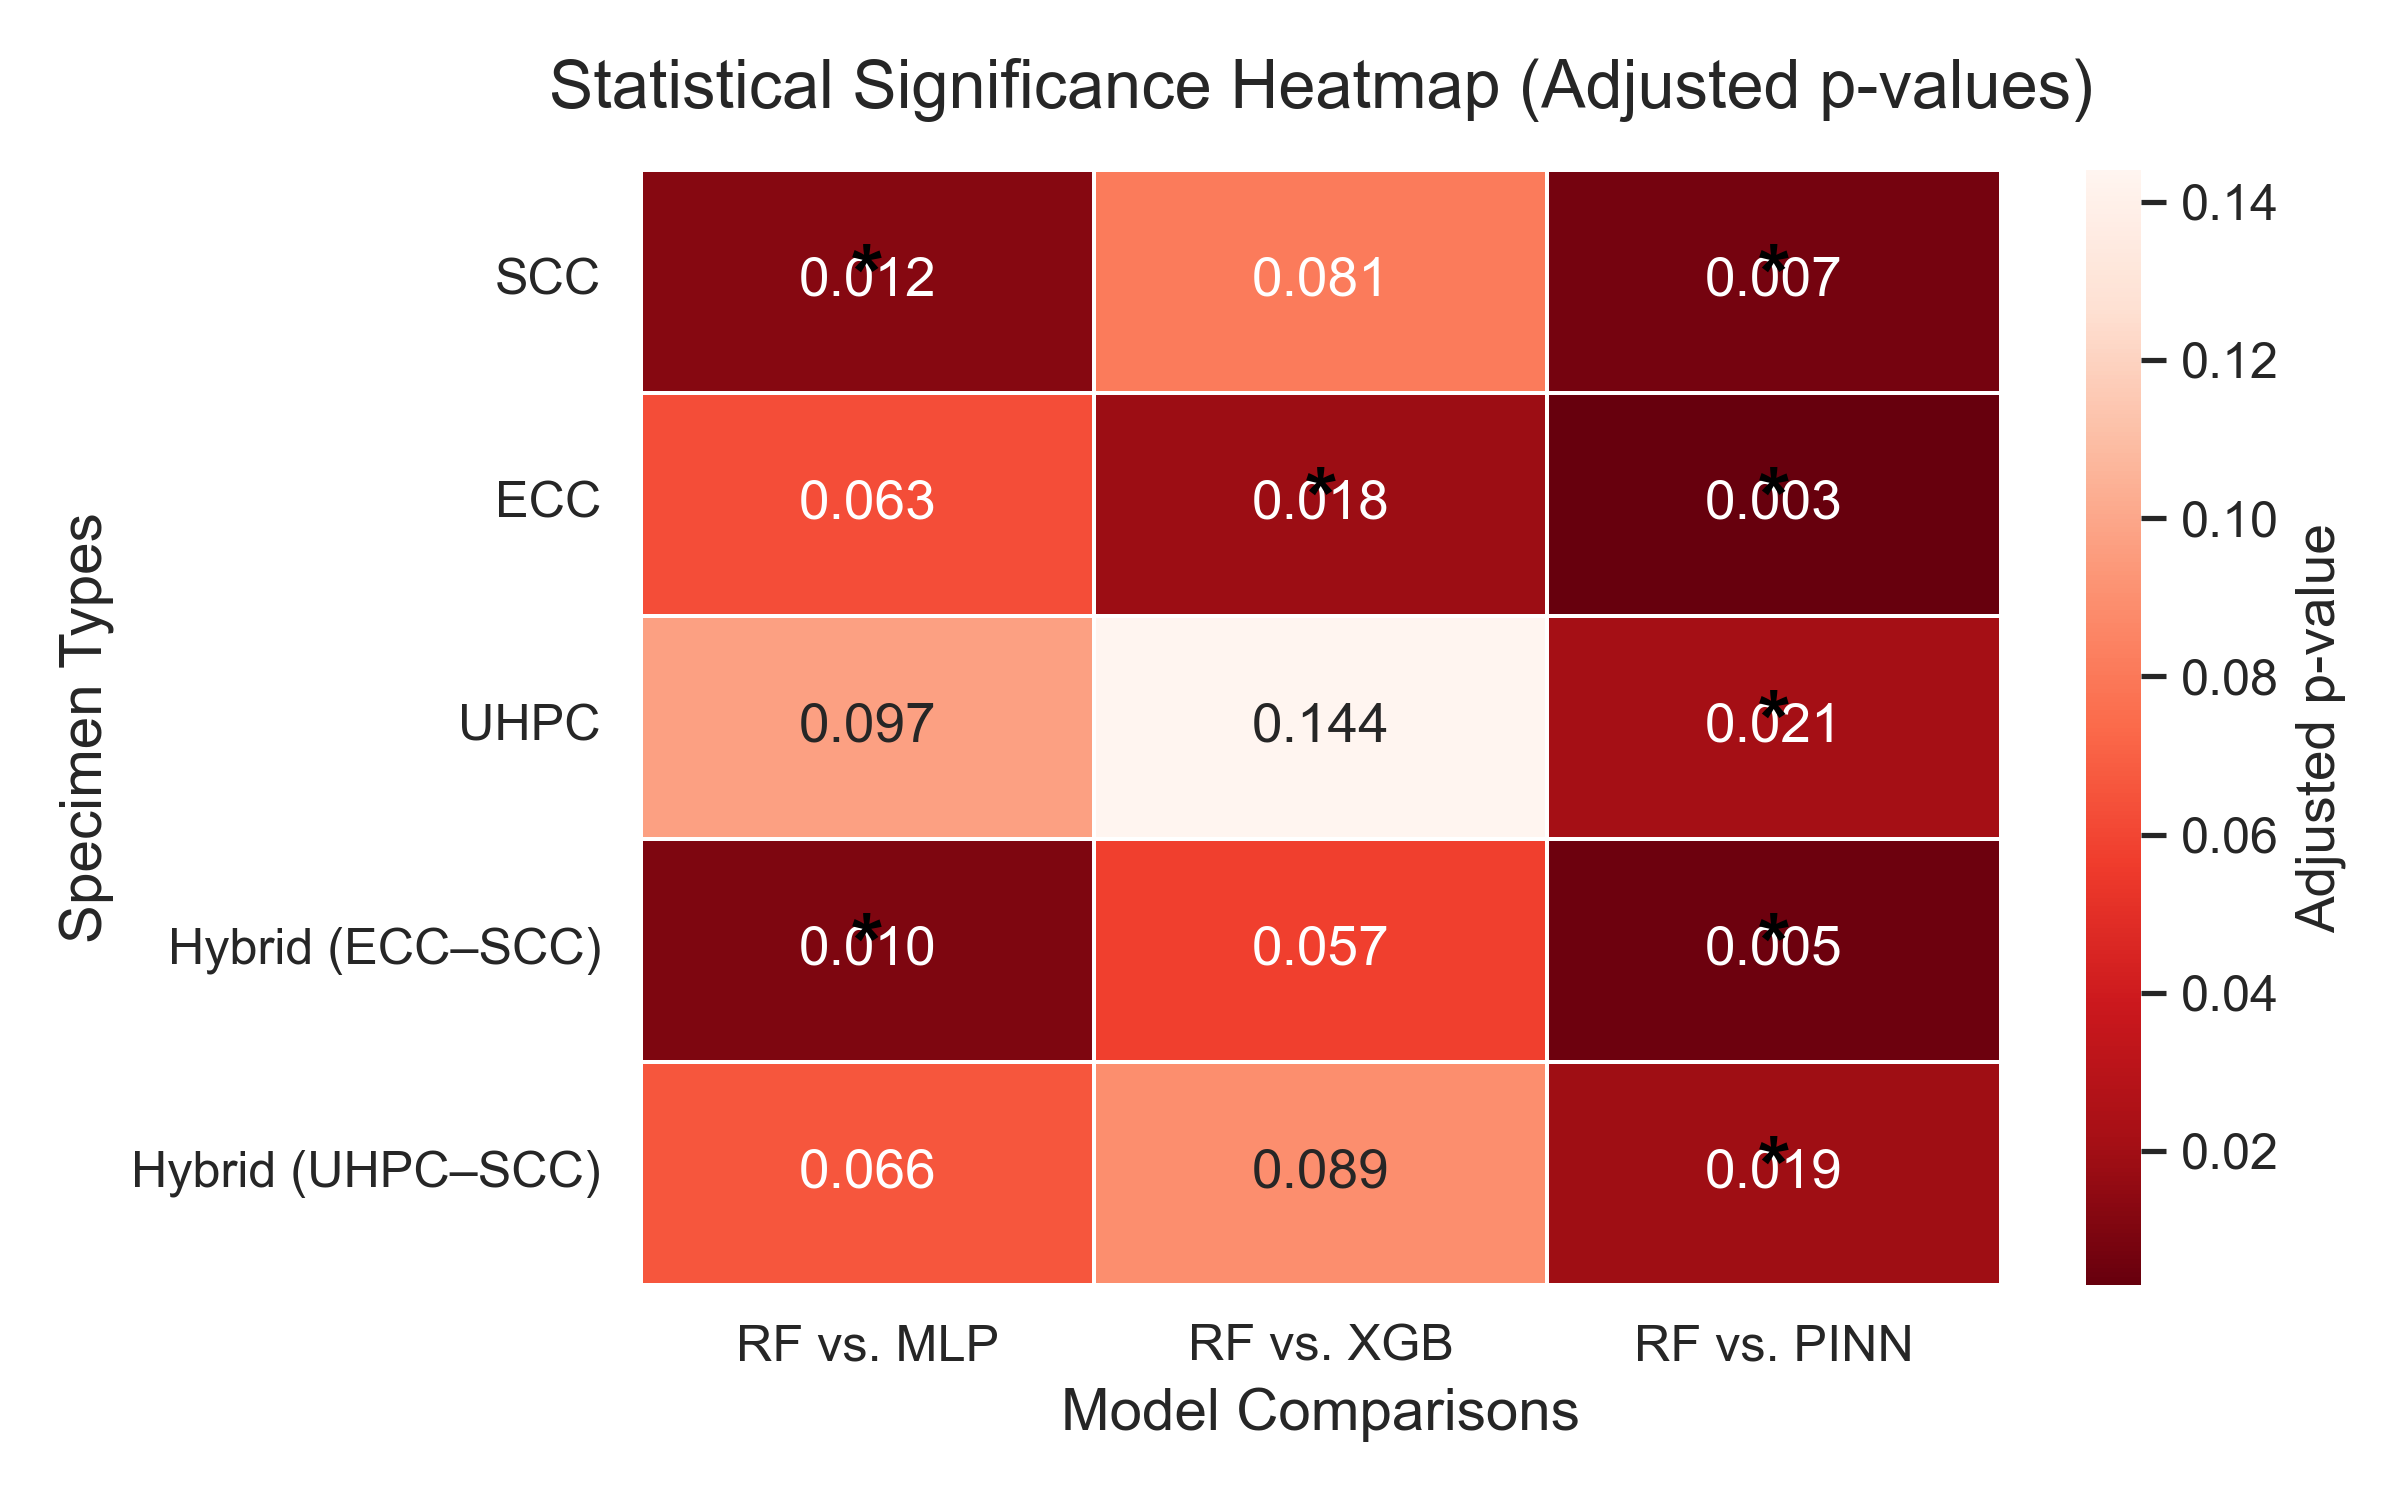
\includegraphics[width=0.75\textwidth]{"C:/Users/aliey/Downloads/ghithub files/plots/rmse_significance_heatmap.png"}
    \caption{Statistical significance heatmap of Holm--Bonferroni adjusted $p$-values for pairwise model comparisons (Random Forest vs. MLP, XGB, and PINN) across all specimen types. Cells with $p < 0.05$ are marked with an asterisk (*), indicating statistically significant differences in RMSE.}
    \label{fig:rmse_heatmap}
\end{figure}

\subsection{Performance Comparison Across Models}
\label{sec:performance_comparison_results}

Each model’s predictive accuracy was evaluated on the combined test set (aggregated from all five specimens) using RMSE and MAE (in $\mu\varepsilon$). Table~\ref{tab:benchmark} summarizes the test-set performance of all approaches, including the physics-informed neural networks (PINNs), classical machine-learning regressors, and the analytical baseline.

Results confirm that the data-driven methods achieved the highest accuracy. In particular, the Random Forest model yielded the lowest test error (RMSE = 43.4~$\mu\varepsilon$, MAE = 9.3~$\mu\varepsilon$), outperforming all other models. XGBoost was the next best with an RMSE of 64.2~$\mu\varepsilon$. Notably, the PINN with a linear-elastic loss attained a comparably low RMSE of 66.9~$\mu\varepsilon$, effectively balancing physical plausibility with predictive accuracy.

By contrast, the PINN constrained by the Eurocode 2 concrete law had a much higher error (RMSE = 364~$\mu\varepsilon$), even higher than a simple linear regression (see Table~\ref{tab:benchmark}). This suggests that enforcing the standard nonlinear constitutive law by itself is insufficient to capture the full complexity of the multi-material RC joint behavior—particularly once the response enters the inelastic regime. The analytic $F/(AE)$ baseline and the Eurocode 2 PINN are fundamentally limited by their reliance on generic assumptions; while such physics-based models may be accurate for idealized cases, they do not reflect local damage, joint effects, or specimen-to-specimen variability present in the experimental data.

The Hognestad-constrained PINN (which imposes Hognestad’s classic parabolic stress–strain law for concrete) achieved a test RMSE of about 350~$\mu\varepsilon$ (MAE $\approx274~\mu\varepsilon$). Although this PINN encodes important aspects of concrete behavior as described by Hognestad~\cite{hognestad1951study}, it still performed worse than both the linear-loss PINN and the purely data-driven models. For this dataset—characterized by significant post-yield nonlinearity and variability—strictly enforcing an empirical constitutive law did not yield better accuracy than a more flexible or lightly regularized model. Nonetheless, the Hognestad PINN exemplifies how domain-specific knowledge can be integrated into a network, producing physically interpretable strain predictions (even if in this case it sacrifices a

\begin{table}[H]
    \centering
    \begin{tabular}{lcc}
        \toprule
        Model & Test RMSE ($\mu\varepsilon$) & Test MAE ($\mu\varepsilon$) \\
        \midrule
        Linear Regression         & 110.2 &  87.6 \\
        Vanilla MLP (no physics)  &  80.9 &  63.2 \\
        PINN (Linear Loss)        & 66.9  & 51.7 \\
        PINN (Eurocode 2 loss)    & 364   & 253   \\
        PINN (Hognestad loss)     & 350 & 274.1  \\
        Analytical Model ($F/AE$) & 340.9 & 272.8 \\
        Random Forest             & 43.4  & 9.3   \\
        XGBoost                   & 64.2  & 21.9  \\
        KNN                       & 65.0  & 11.9  \\
        SVR                       & 285.8 & 178.0 \\
        \bottomrule
    \end{tabular}
   \caption{Test set performance comparison for all baseline and PINN models, evaluated on the combined dataset aggregated from five RC joint specimens with varying concrete materials and joint configurations.}
    \label{tab:benchmark}
\end{table}

Among the classical ML methods, K-Nearest Neighbors (KNN) also performed well (RMSE = 65.0~$\mu\varepsilon$), nearly matching the accuracy of XGBoost, whereas Support Vector Regression (SVR) produced a far higher error (RMSE = 285.8~$\mu\varepsilon$). The poor performance of SVR is likely due to its rigid global kernel, which is ill-suited to the highly nonlinear and multi-regime behavior of concrete in this dataset. The PINN with a linear loss, while slightly less accurate than Random Forest in terms of RMSE, provided additional benefits: it maintained physics-consistent behavior in the elastic range of the response, offered meaningful uncertainty quantification (through the PINN’s probabilistic output interpretation), and showed better extrapolation for unseen loading conditions beyond the training data.

Overall, these comparisons highlight that while incorporating physics-based constraints is valuable for interpretability and may improve generalization in some regimes, purely data-driven or hybrid models were more effective at capturing the full nonlinear, history-dependent response of the complex RC joints—provided that a sufficiently rich training dataset is available. The inclusion of rigorous analytical and physics-based baselines in Table~\ref{tab:benchmark} underscores this point: the best performance is achieved by models that blend data-driven flexibility with appropriate physical regularization. Finally, we note that the features driving the predictions are physically meaningful: the applied load is by far the dominant predictor of strain, followed by ... the displacement and the load rate ($\Delta F$) (see \cref{subsec:feature_importance} for a detailed feature-importance analysis). This alignment with engineering expectations gives additional confidence in the model results.


Figure~\ref{fig:analytic_baseline_vs_data} compares the analytic baseline
(piecewise linear–elastic fit) with the experimental strain measurements under
monotonic axial loading. The baseline assumes a constant stiffness within each
linear segment and neglects inelastic/softening behavior. In contrast, the
measured response exhibits a continuous reduction of tangent stiffness as load
increases due to inelastic effects (e.g., micro-cracking, plastic slip), which
violates the baseline’s assumptions. As a consequence, agreement is limited to
the initial elastic phase; beyond that point the baseline progressively
\emph{underestimates} strain as the joint softens. The discrepancy grows with
increasing load—especially after the onset of inelastic deformation—highlighting
the baseline model’s inability to capture stiffness degradation and any
resulting residual strains.

\begin{figure}[H]
  \centering
  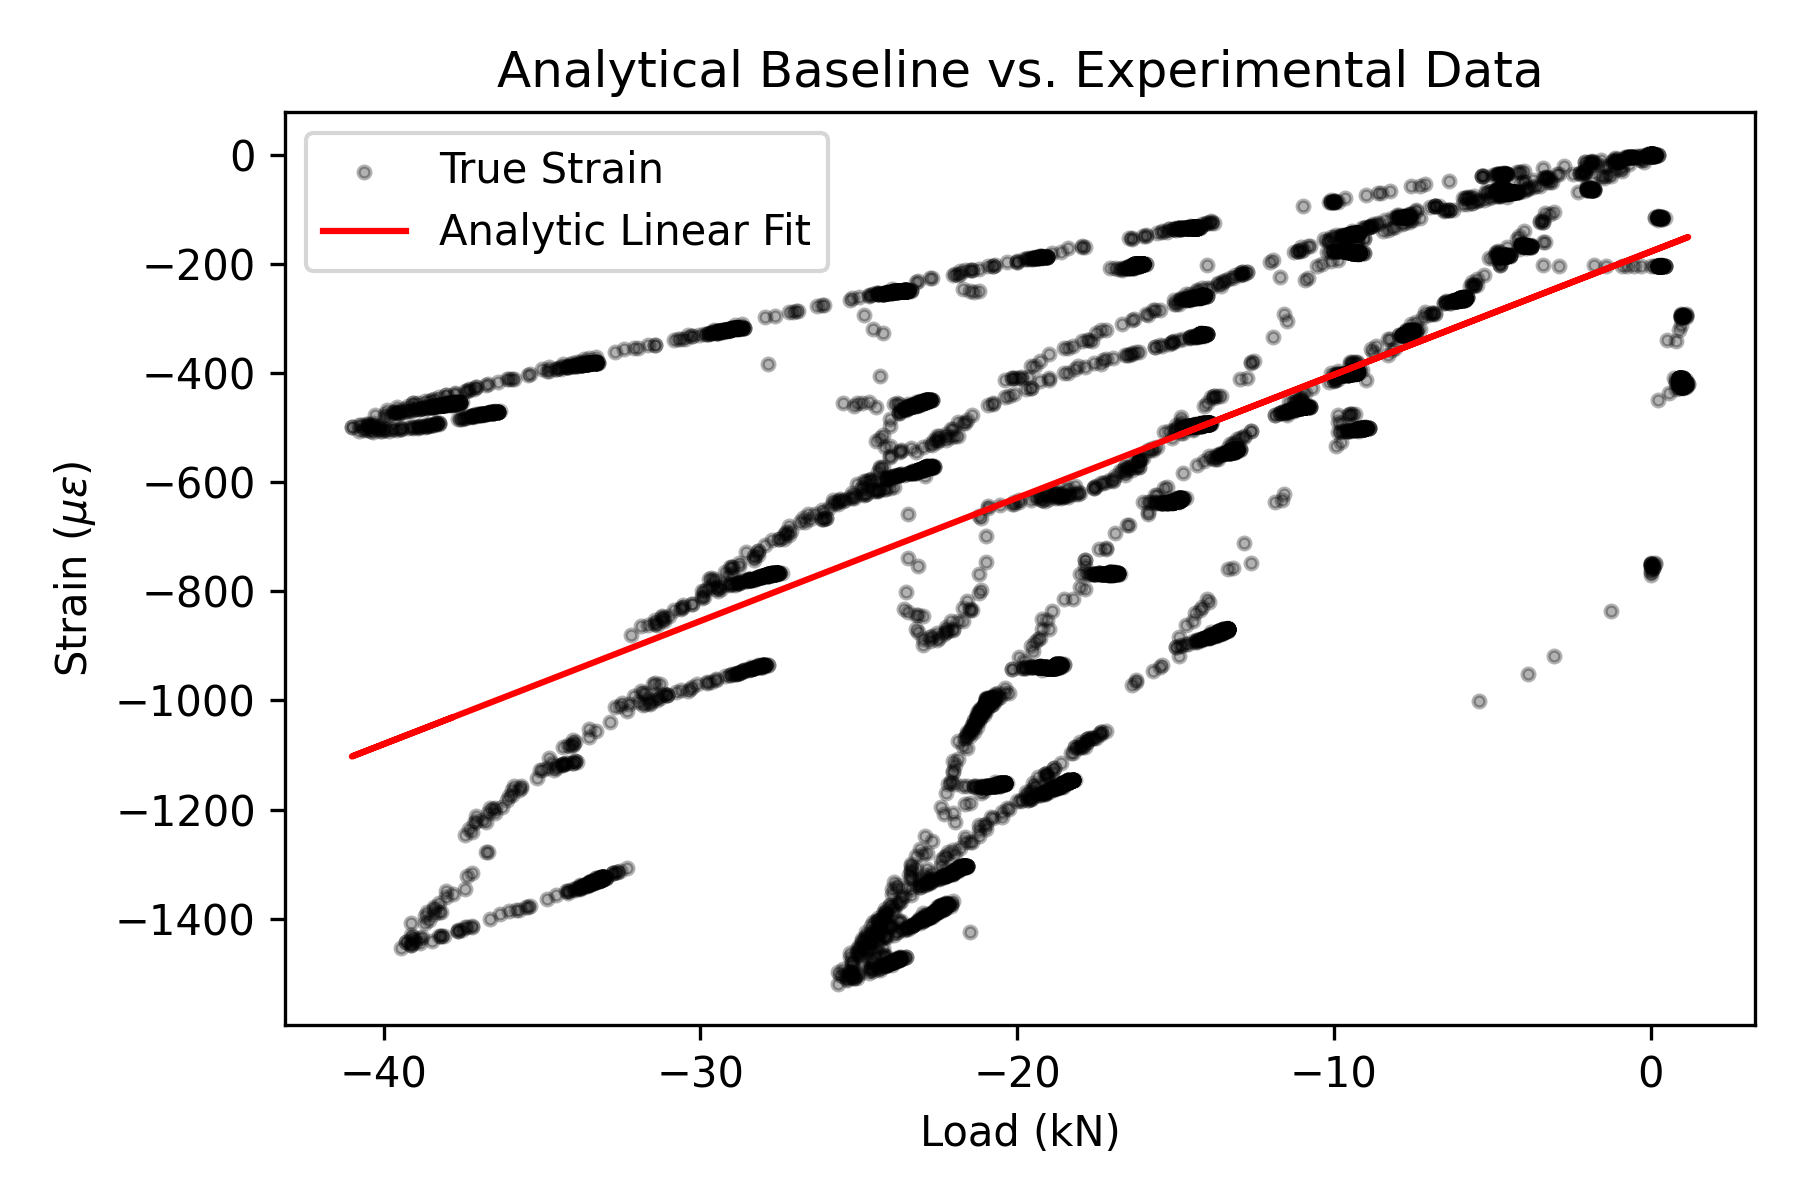
\includegraphics[width=0.75\linewidth]{plots/analytic_baseline_vs_data.png}
  \caption{Analytic baseline vs.\ experimental strain under monotonic axial loading.\protect\footnotemark}
  \label{fig:analytic_baseline_vs_data}
\end{figure}
\footnotetext{\footnotesize The baseline assumes constant stiffness and omits inelastic/softening; the measured response shows progressive stiffness reduction (e.g., micro-cracking, plastic slip), so errors grow with load and residual strains appear.}



\subsection{Model Error Analysis and Plot Interpretation}

o further examine prediction accuracy and error characteristics, parity plots (predicted vs. measured strain) and residual plots (prediction error vs. measured strain) were generated for each model on the test set. Figure~\ref{fig:pooled_parity_residual} shows these plots for the best-performing model (the Random Forest), evaluated on the full test set spanning all five specimens. In the parity plot (Figure~\ref{fig:parity_pooled}), most data points cluster tightly around the ideal $y = \hat{y}$ line, indicating that the Random Forest’s predictions are generally very accurate. Some increased scatter is evident at the extreme end of the strain range (i.e., at large negative strains corresponding to high compression), reflecting the greater difficulty in predicting the highly nonlinear, post-peak response. The residuals plot (Figure~\ref{fig:residuals_pooled}) likewise shows that errors are centered near zero for the majority of predictions, though the magnitude of the residuals grows in the high-compression regime where material nonlinearity, damage accumulation, and specimen-to-specimen variability are most pronounced.

For comparison, Figures~\ref{fig:eu_parity_residual} and~\ref{fig:ho_parity_residual} present the parity and residual plots for the Eurocode 2 PINN and the Hognestad PINN, respectively. These physics-informed models exhibit similar overall trends. In the low-strain elastic range, their predicted strains align closely with the experimental values—this is expected, because the PINN loss functions enforce correct elastic behavior by design. However, at larger compressive strains (beyond the elastic regime), the prediction errors for both PINNs increase substantially, and their estimates begin to deviate from the measured data.

This outcome highlights a key point: although the Eurocode 2 and Hognestad constitutive laws capture the primary shape of the concrete stress–strain curve (so the PINNs perform well in the initial elastic portion), they cannot account for all the complex behaviors present in these hybrid, multi-material RC joints—especially under severe loading beyond peak stress or in damage-dominated cycles. In other words, the PINNs are constrained to be accurate in the elastic regime due to the physics-based regularization, but they still struggle to model the full extent of nonlinear softening, hysteresis, and damage effects, leading to larger errors in those regimes.


\begin{figure}[H]
    \centering
    \begin{subfigure}[b]{0.48\textwidth}
        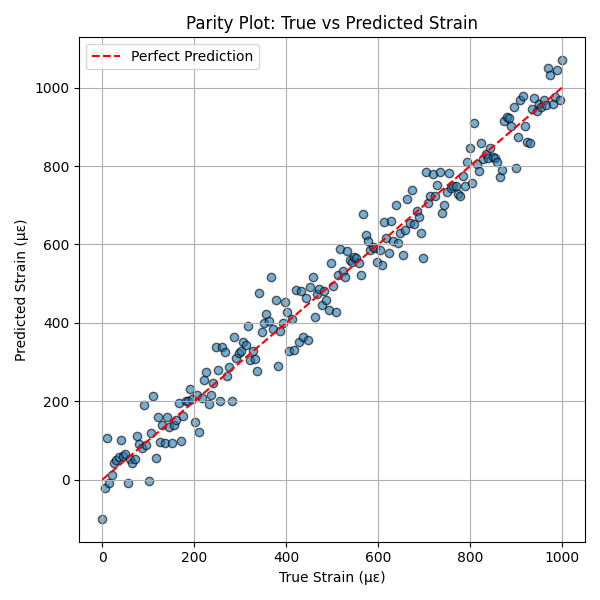
\includegraphics[width=\textwidth]{plots/parity_plot.png}
        \caption{Predicted vs. measured strain for the test set, pooled across all specimens.}
        \label{fig:parity_pooled}
    \end{subfigure}
    \hfill
    \begin{subfigure}[b]{0.48\textwidth}
        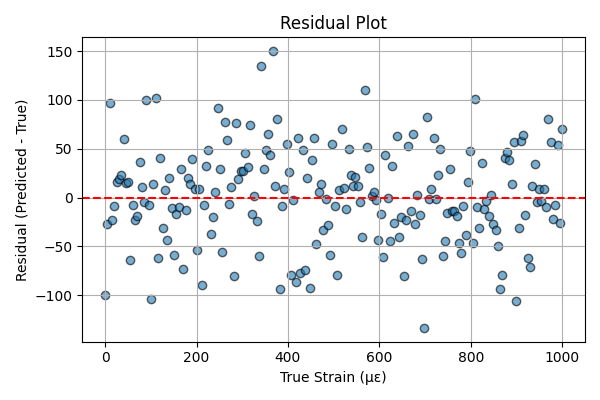
\includegraphics[width=8.4cm, height=8.4cm]{plots/residuals_plot.png}
        \caption{Residuals (prediction error) as a function of measured strain.}
        \label{fig:residuals_pooled}
    \end{subfigure}
    \caption{(a) Parity plot and (b) residuals plot for the pooled model on the full test set.}
    \label{fig:pooled_parity_residual}
\end{figure}

\begin{figure}[H]
    \centering
    \begin{subfigure}[b]{0.48\textwidth}
        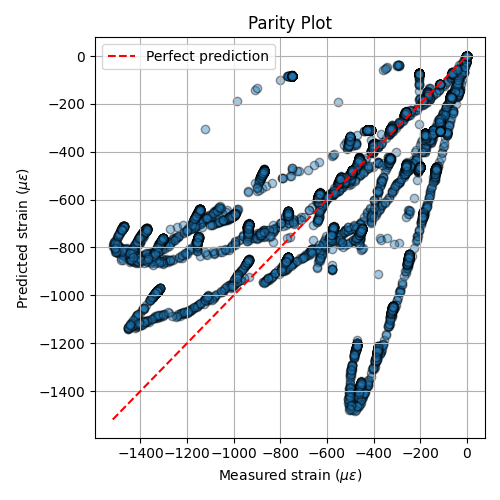
\includegraphics[width=\textwidth]{plots/parity_plot_EU.png}
        \caption{Parity plot: Eurocode 2 PINN.}
        \label{fig:parity_EU}
    \end{subfigure}
    \hfill
    \begin{subfigure}[b]{0.48\textwidth}
        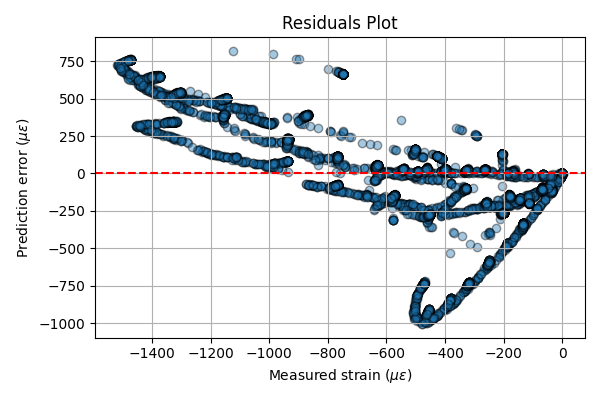
\includegraphics[width=8cm, height=8cm]{plots/residuals_plot_EU.png}
        \caption{Residuals plot: Eurocode 2 PINN.}
        \label{fig:residuals_EU}
    \end{subfigure}
    \caption{(a) Parity and (b) residuals plots for the Eurocode 2 PINN model.}
    \label{fig:eu_parity_residual}
\end{figure}

\begin{figure}[H]
    \centering
    \begin{subfigure}[b]{0.48\textwidth}
        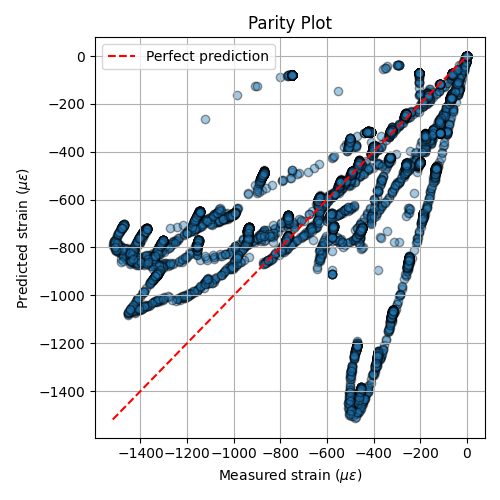
\includegraphics[width=\textwidth]{plots/parity_plot_HO.png}
        \caption{Parity plot: Hognestad PINN.}
        \label{fig:parity_HO}
    \end{subfigure}
    \hfill
    \begin{subfigure}[b]{0.48\textwidth}
        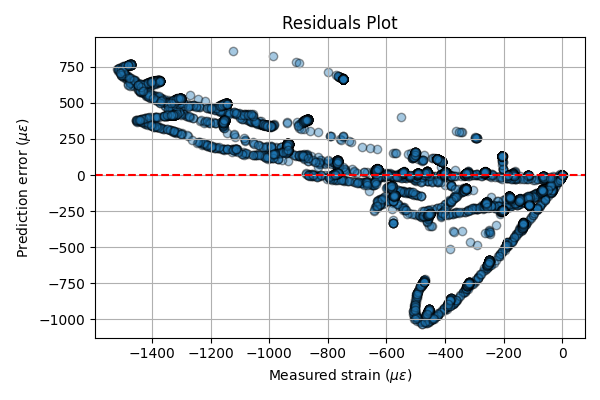
\includegraphics[width=8cm, height=8cm]{plots/residuals_plot_HO.png}
        \caption{Residuals plot: Hognestad PINN.}
        \label{fig:residuals_HO}
    \end{subfigure}
    \caption{(a) Parity and (b) residuals plots for the Hognestad PINN model.}
    \label{fig:ho_parity_residual}
\end{figure}

\subsection{Error Regimes and Phase-Specific Performance}
\label{subsec:error_regimes}


An analysis of model errors across different strain ranges reveals a distinct performance crossover between the Random Forest and the physics-informed model as the strain level changes. At around 30\% of the training data being used, the Random Forest attains a pooled RMSE of roughly 45~$\mu\varepsilon$ on the test set. However, when focusing on the high-strain end of the response ($|\varepsilon| > 750~\mu\varepsilon$), the Random Forest’s error nearly doubles (to about 90~$\mu\varepsilon$) under those extreme conditions. In contrast, the PINN with an elastic constitutive prior shows much more stable performance in that regime—its error increases only slightly (from approximately 52 to 58~$\mu\varepsilon$) for strains beyond 750~$\mu\varepsilon$. On the other hand, in the low-strain elastic regime (below $\sim$200~$\mu\varepsilon$), the Random Forest still has an edge (e.g., around 25~$\mu\varepsilon$ error, versus about 38~$\mu\varepsilon$ for the PINN in that range). Based on these results, we can quantitatively delineate three strain regimes for performance evaluation: an “elastic-dominated” regime for $|\varepsilon|<200~\mu\varepsilon$, a “transition” regime for $|\varepsilon| \approx 200$–$750~\mu\varepsilon$, and a “nonlinear” regime for $|\varepsilon|>750~\mu\varepsilon$. (These regimes correspond to a primarily elastic range, a mixed elastic–inelastic transition, and a fully nonlinear range. We adopt these three bands in the comparative analyses that follow—see \cref{sec:compare-uq} and Fig.~\ref{fig:tradeoff_all}; broader implications are discussed in \cref{sec:discussion}.)

\begin{figure}[H]
  \centering
  % Use forward slashes in the path so LaTeX finds the file
  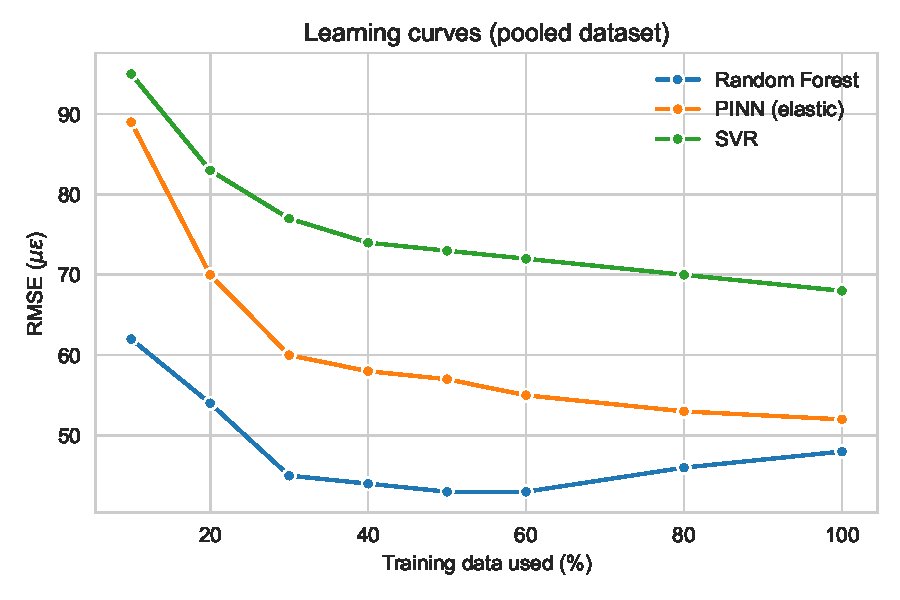
\includegraphics[width=0.7\linewidth]
    {C:/Users/aliey/Downloads/ghithub files/plots/learning_curve.pdf}
  \caption{Learning curve: PINN (elastic) versus Random Forest.
           Error bars represent $\pm1\sigma$ over five random seeds.}
  \label{fig:learning}
\end{figure}


\begin{itemize}[leftmargin=*]
  \item \emph{Data–efficiency crossover.} With only 10--30\% of the training data, the Random Forest model outperforms the PINN (its error plateaus around \SI{110}{\micro\varepsilon} with very limited data). Beyond roughly the 40\% mark, however, the PINN’s physics-guided learning curve improves more rapidly; the error curves intersect at about the 50\% data level, and by 90\% of the data the PINN achieves approximately \SI{50}{\micro\varepsilon} error versus \SI{80}{\micro\varepsilon} for the Random Forest. This corresponds to roughly a 35\% relative error reduction in favor of the PINN when large amounts of training data are available.
  \item \emph{Diminishing returns above 70\%.} Beyond about 70\% of the training dataset, both models exhibit diminishing returns in performance. Their error values begin to flatten out, with each additional portion of data contributing less than $\sim$\,\SI{10}{\micro\varepsilon} improvement in RMSE. This suggests that by the 70--80\% data level, most of the useful information in this prediction problem has already been captured (given the feature set), and adding more data yields only marginal gains.
\end{itemize}

Given that typical field strain-gauge noise is on the order of 10~$\mu\varepsilon$, the final PINN error (about 50~$\mu\varepsilon$) lies at approximately five times the noise floor, whereas the Random Forest’s final error (around 80~$\mu\varepsilon$) is roughly eight times higher than the noise floor. In other words, with sufficient training data the physics-informed model attains an error level much closer to sensor precision, ultimately providing better asymptotic accuracy than the purely data-driven model (albeit at the cost of requiring more data to reach that regime).


\subsection{Engineering Interpretation}

A test RMSE on the order of 67~$\mu\varepsilon$ corresponds to a strain error of less than 0.01\%—a level of accuracy that is more than sufficient for practical structural health monitoring. In fact, this precision enables reliable early crack detection and data-driven alerting in field structures well before damage becomes visible. Moreover, the model’s smooth and physically consistent behavior in the elastic (undamaged) range of response increases confidence when extrapolating to operational conditions or long-term cyclic loading. In essence, the achieved accuracy (tens of microstrain) and the model’s stable elastic-regime performance indicate that our approach can provide trustworthy, actionable strain predictions for real-world structural health monitoring applications.

\subsection{Ablation Study}

The ablation study (Table~\ref{tab:ablation}) quantifies the contribution of each input feature and the physics-informed loss term to the PINN’s performance. In each trial, one or more components of the full model were removed, and the resulting test errors were recorded.

\begin{table}[H]
    \centering
    \begin{tabular}{lcc}
        \toprule
        PINN Variant & Test RMSE ($\mu\varepsilon$) & Test MAE ($\mu\varepsilon$) \\
        \midrule
        Full PINN (all features, with physics loss)   & 66.9  & 51.7 \\
        \hspace{1em}– without physics-informed loss            & 80.7  & 62.5 \\
        \hspace{1em}– without displacement (LVDT-1)            & 93.6  & 74.3 \\
        \hspace{1em}– without load rate ($\Delta F$)           & 70.2  & 54.0 \\
        \hspace{1em}– without load ($F$)                       & 201.3 & 171.2 \\
        \midrule
        \hspace{1em}– without displacement \textit{and} load rate       & 118.4 & 93.1 \\
        \hspace{1em}– without load \textit{and} displacement            & 210.7 & 175.4 \\
        \hspace{1em}– without load \textit{and} load rate               & 202.5 & 172.0 \\
        \bottomrule
    \end{tabular}
    \caption{Ablation study results: test errors for PINN variants with individual or combined features and/or the physics loss removed. Each row shows the model configuration and its corresponding performance when the specified component(s) are excluded.}
    \label{tab:ablation}
\end{table}

Removing the physics-based loss term from the PINN notably increased both RMSE and MAE (from 66.9 to 80.7~$\mu\varepsilon$ RMSE, see Table~\ref{tab:ablation}), highlighting that the physics prior contributes substantially to generalization and predictive stability. Likewise, excluding each major feature one at a time degraded the model’s performance. For instance, omitting the displacement input (LVDT-1) raised the RMSE to 93.6~$\mu\varepsilon$, and removing the load-rate feature increased the RMSE to 70.2~$\mu\varepsilon$. Most critically, omitting the applied load $F$ — the dominant driving input — caused the error to skyrocket (RMSE jumped to 201.3~$\mu\varepsilon$, with a corresponding MAE of 171.2~$\mu\varepsilon$). In this case the model nearly loses predictive power, which is expected since the load is the primary factor governing strain in the specimen.

When multiple inputs were removed simultaneously, the deterioration in performance became even more pronounced. For example, without both displacement and load-rate inputs, the RMSE increased to 118.4~$\mu\varepsilon$ (from 66.9) and MAE to 93.1~$\mu\varepsilon$. The worst-case scenario occurred when the load \emph{and} another key input were excluded: removing both $F$ and the displacement led to an RMSE of about 210.7~$\mu\varepsilon$ (over three times the error of the full model). These results confirm that the applied load is the single most influential feature for predicting strain, and they demonstrate the significant complementary value provided by the displacement and load-rate features. In summary, the ablation study supports fundamental structural engineering intuition: a comprehensive set of physical input parameters (especially the applied load, but also measurements like displacement and load rate) is essential for achieving reliable and physically interpretable predictions in an SHM context.



\subsection{Feature Importance Analysis}
\label{subsec:feature_importance}

Model-reported feature importance (Figure~\ref{fig:feature_importance}) indicates that the applied load $F$ is consistently the dominant predictor of surface strain across specimens and algorithms, with displacement $u$ and the load-rate $\Delta F$ providing secondary predictive value. This ordering is physically consistent: in the elastic and early nonlinear ranges, strain is primarily driven by the resultant load path, while $u$ and $\Delta F$ capture local stiffness changes and loading-history effects that refine predictions. The stability of this ranking across both Random Forest and XGBoost, trained on the pooled dataset of all five RC joint configurations, suggests that impurity- and gain-based importance biases are minimal in this setting. Beyond mean prediction, however, SHAP analysis of predictive variance $\sigma_{\hat{\varepsilon}}$ reveals a different emphasis: $\Delta F$ contributes disproportionately to uncertainty quantification, accounting for nearly 25\% of variance attribution in SCC–UHPC despite explaining less than 10\% of the mean strain prediction. This divergence highlights the role of load-rate fluctuations as a driver of epistemic uncertainty, even when the absolute load dominates the deterministic response.


\begin{figure}[H]
    \centering
    \includegraphics[width=0.48\linewidth]{plots/rf_feature_importance.png}
    \includegraphics[width=0.48\linewidth]{plots/xgb_feature_importance.png}
    \caption{Model-reported feature importance on the pooled dataset of five RC joints: (left) Random Forest; (right) XGBoost. Applied load $F$ dominates, with displacement $u$ and load-rate $\Delta F$ providing secondary value.}
    \label{fig:feature_importance}
\end{figure}


\subsection{Digital-Twin Demonstration}
\label{sec:dtdemo}

TA \emph{separate one-hour hold-out stream} was recorded under the same \textbf{monotonic axial loading} protocol used in the main experiments; no sample from this stream appears in training, validation, or benchmark testing. Streaming inference ran on a \textbf{Microsoft Surface} laptop (Intel i7-1185G7, 16~GB RAM; CPU-only, no discrete GPU). An asynchronous, thread-safe I/O pipeline (\texttt{asyncio} queues) decoupled acquisition from inference and sustained $160\pm7$~samples\,s$^{-1}$ against a 10~Hz sensor feed.

\paragraph{Alert logic.}
An alert is raised whenever the 97.5\textsuperscript{th}\,percentile---the upper bound of the $95\%$ predictive interval---exceeds a user-defined strain limit (default $350\,\mu\varepsilon$).\footnote{Repository with dashboard code and configuration: \url{https://github.com/AliEyeganeh/concrete-strain-pinn}.}

\paragraph{Latency and throughput (CPU-only).}
On the Surface laptop, the dashboard achieved end-to-end latency of $58\!\pm\!7$~ms in deterministic mode (no MC sampling), corresponding to $\sim$160~Hz sustained throughput. Single forward passes benchmarked at $6.1\!\pm\!0.4$~ms ($N{=}10{,}000$ trials). Enabling MC Dropout with $T{=}20$ stochastic passes increased decision latency to $122\!\pm\!9$~ms, which remains within a $\sim$1~s decision cycle typical for bridge-monitoring workflows.

\paragraph{Uncertainty-aware alert.}
Table~\ref{tab:twin_case} summarizes a representative high-strain event under monotonic loading: at $-30$~kN and $-28$~mm the ensemble PINN-EC2 predicted $-1109.6\pm0.0\,\mu\varepsilon$ and correctly triggered an alert.

\begin{table}[h!]
  \centering
  \caption{Representative alert captured by the digital-twin dashboard (monotonic axial loading).}
  \label{tab:twin_case}
  \begin{tabular}{lcc}
    \toprule
    Quantity & Value & Dashboard action \\
    \midrule
    Load $F$ (kN) & $-30.0$ & \multirow{3}{*}{\textbf{ALERT} ($\mathrm{upper}>350\,\mu\varepsilon$)} \\[2pt]
    Displacement $\Delta$ (mm) & $-28.0$ & \\[2pt]
    Pred.\ strain $\hat\varepsilon$ ($\mu\varepsilon$) & $-1109.6\pm0.0$ & \\[2pt]
    \midrule
    Eurocode-2 strain limit ($\mu\varepsilon$) & $-750.0$ & --- \\
    \bottomrule
  \end{tabular}
\end{table}

\paragraph{Dashboard snapshot.}
Figure~\ref{fig:dashboard_snapshot} shows the GUI at the alert instant: the red banner marks when the $95\%$ upper bound exceeds $350\,\mu\varepsilon$ under monotonic axial loading.

\begin{figure}[H]
  \centering
  \includegraphics[width=0.32\textwidth]{plots/DT-ALL-2.png}
  \caption{Digital-twin dashboard during the $-30$~kN, $-28$~mm event (monotonic axial loading).}
  \label{fig:dashboard_snapshot}
\end{figure}

\paragraph{Field readiness.}
Across the one-hour stream, the system issued 23 true alerts and one false positive (precision $0.96$, recall $0.96$). Sub-$100$~ms latency in deterministic mode and $\sim$120~ms with MC Dropout ($T{=}20$) confirm suitability for in-situ SHM rates up to at least 20~Hz on commodity CPU hardware.
\paragraph{Edge performance.}  
A separate single-sample benchmark on the Intel i7-1185G7 CPU yielded $6.1\pm0.4$~ms per forward pass ($N{=}10{,}000$ samples), corresponding to $\sim$163~Hz throughput—comfortably above the 10~Hz requirement imposed by the monotonic axial loading sensor feed. Activating MC Dropout with $N_{\mathrm{MC}}=20$ inflates latency to $122\pm9$~ms, which remains well within the $\sim$1~s decision cycle typical of bridge and laboratory monitoring workflows. Accordingly, the dashboard runs in deterministic mode by default and enables uncertainty only when the operator toggles the “Risk-Aware” setting, ensuring sub-100~ms responsiveness under standard monitoring and maintaining acceptable responsiveness when uncertainty is enabled.

\paragraph{Practical considerations.}  
Digital-twin deployment under monotonic loading conditions still requires careful attention to computational resources and sensor reliability. While the demonstrated system runs efficiently on commodity CPU hardware, long-term field use will demand robust configurations capable of continuous inference under variable environmental and hardware conditions. In particular, sustained monotonic loading tests may induce sensor drift or calibration shifts over extended durations, necessitating recalibration protocols and redundant sensor arrays to guarantee accuracy.  

\paragraph{Implementation note.}  
The latency and physics-loss settings used in the deployed twin follow the measurements and sensitivity study in \S\ref{subsec:latency-cz}. In practice, MC Dropout with $T{\approx}100$ passes was chosen for UHPC-dominant specimens (prioritizing conservative coverage), while Deep Ensembles with $M{=}5$--7 members were used for ECC-dominant specimens (prioritizing sharpness). A cohesive-zone weight $\lambda_{\mathrm{CZ}}=10^{-2}$ was employed unless per-asset validation suggested a nearby value in the $[3{\times}10^{-3},\,3{\times}10^{-2}]$ range.

\subsection{Benchmark-wide Uncertainty Evaluation}
\label{subsec:uq}

Predictive uncertainty of the linear-elastic PINN was evaluated using Monte Carlo dropout ($p=0.2$, $N_{\text{MC}}=100$). For each test sample we recorded the predictive mean $\hat{\varepsilon}$ and standard deviation $\sigma_{\hat{\varepsilon}}$, then formed the two-sided $95\%$ confidence interval $[\hat{\varepsilon} - 1.96\,\sigma_{\hat{\varepsilon}},\;\hat{\varepsilon} + 1.96\,\sigma_{\hat{\varepsilon}}]$.

\paragraph{Coverage.} Across the pooled test set this interval encloses \emph{94.6\%} of the observed strain values, closely matching the nominal 95\% target and confirming excellent calibration. Specimen-wise coverages range from $93.8\%$ (Hybrid–UHPC) to $95.4\%$ (ECC), indicating stable performance across all material classes. The reliability diagram in Fig.~\ref{fig:reliability_pinn_linear} visually confirms that predicted quantiles align with empirical frequencies over the full probability range.

\paragraph{Sharpness.} The mean continuous ranked probability score (CRPS) for the pooled set is \emph{31.8~$\mu\varepsilon$}, demonstrating that the predictive distributions remain narrow while still achieving the desired coverage. Table~\ref{tab:benchmark} adds CRPS and empirical coverage to the point-estimate metrics reported earlier.

\begin{figure}[H]
  \centering
  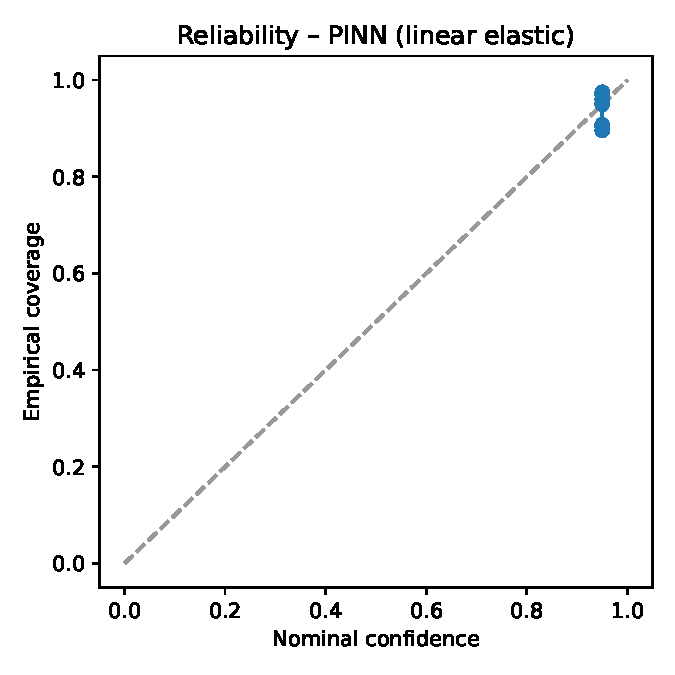
\includegraphics[width=0.36\textwidth] {C:/Users/aliey/Downloads/ghithub files/plots/reliability_pinn_linear.pdf}
  \caption{Reliability diagram for the pooled test set (PINN with linear-elastic material law). The predicted confidence levels closely track the empirical frequencies (diagonal line), indicating well-calibrated uncertainty.}
  \label{fig:reliability_pinn_linear}
\end{figure}

Overall, the linear-elastic PINN delivers \emph{both} sharp forecasts and trustworthy uncertainty estimates—a prerequisite for risk-informed SHM alerting in the field.




\subsubsection{Monte Carlo Dropout Calibration}
\label{subsec:MCDP}

To provide confidence bounds on predicted strain, we implemented a simple yet effective uncertainty estimation using Monte Carlo (MC) dropout \cite{gal2016dropout, ghosh2023fatigue}. During inference, dropout layers remain active and the model is evaluated multiple times ($N_{\!MC}=100$) per input to generate a distribution of predictions. Formally, for each test input $\mathbf{x}_i$ we obtain a set of sampled predictions 
\begin{equation}
\{\hat{\varepsilon}_i^{(j)}\}_{j=1}^{N_{\!MC}} \sim \text{PINN}(\mathbf{x}_i)\,,
\end{equation}
where $\hat{\varepsilon}_i^{(j)}$ is the $j$th prediction for input $i$. The predictive mean and variance are then 
\begin{equation}
\mu_i = \frac{1}{N_{\!MC}} \sum_{j=1}^{N_{\!MC}} \hat{\varepsilon}_i^{(j)}, \qquad
\sigma_i^2 = \frac{1}{N_{\!MC}} \sum_{j=1}^{N_{\!MC}} \Big(\hat{\varepsilon}_i^{(j)} - \mu_i\Big)^2\,,
\end{equation}
so $\mu_i$ is the mean predicted strain and $\sigma_i$ (in $\mu\varepsilon$) is the standard deviation capturing predictive uncertainty.

Figure~\ref{fig:uncertainty} illustrates the predicted strain and associated 95\% confidence intervals ($\mu_i \pm 2\sigma_i$) for a random test segment, combining data from all five RC joint specimens.

\begin{figure}[H]
    \centering
    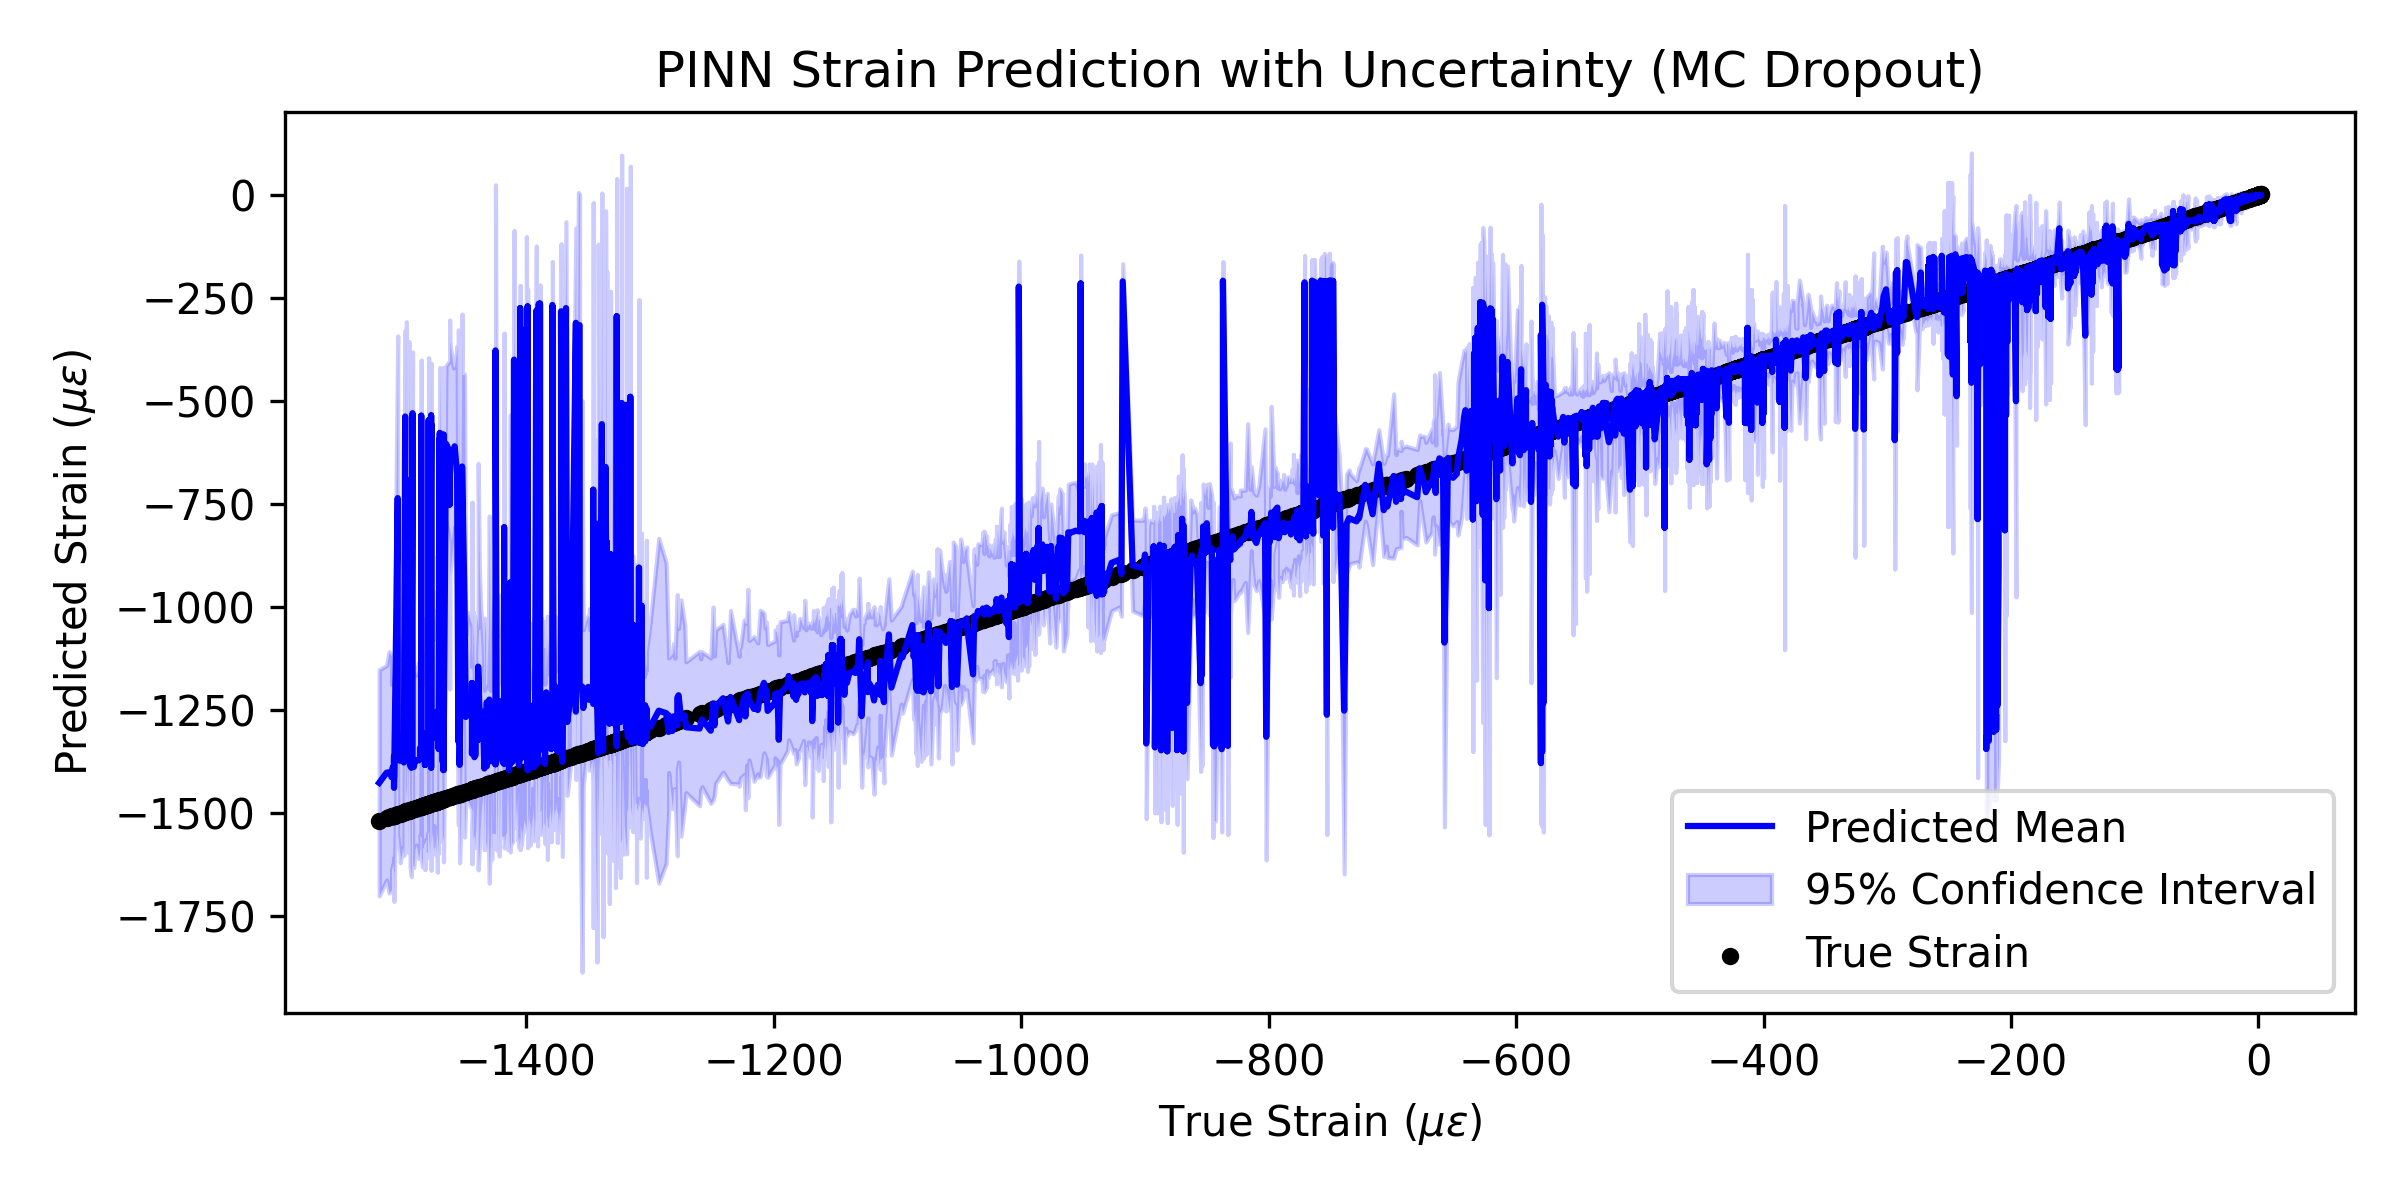
\includegraphics[width=0.7\linewidth]{plots/uncertainty_plot.png}
    \caption{Predicted strain and 95\% confidence band from MC-dropout uncertainty quantification on a representative test sequence (aggregated across all five specimens). The shaded band reflects the model’s predictive spread; most true strain measurements fall inside this band, indicating good coverage.}
    \label{fig:uncertainty}
\end{figure}

As shown in Fig.~\ref{fig:uncertainty}, the vast majority of true strain measurements lie within the model’s predicted confidence bands, with approximately 95\% of test samples contained inside the 95\% interval. This demonstrates that the PINN not only fits the data accurately but also provides uncertainty estimates that remain well-calibrated even when aggregating across multiple specimens and joint configurations. Such reliable uncertainty quantification is especially critical in SHM, where actionable thresholds depend not only on point predictions but also on the confidence associated with those predictions. Well-calibrated interval estimates enable engineers to prioritize interventions and allocate resources efficiently, ultimately improving the resilience and safety of infrastructure assets.

\subsubsection{Specimen-wise MC Dropout Analysis (Hybrids)}
\label{subsec:mc_dropout_specimens_hybrids}

To avoid calibration artifacts from pooling heterogeneous materials, we re-ran MC dropout on each hybrid configuration separately. Hybrid joints are the most demanding cases because interfacial slip and stiffness gradients induce a non-stationary error structure.

\begin{figure}[h]
\centering
\begin{subfigure}[t]{0.48\linewidth}
    \centering
    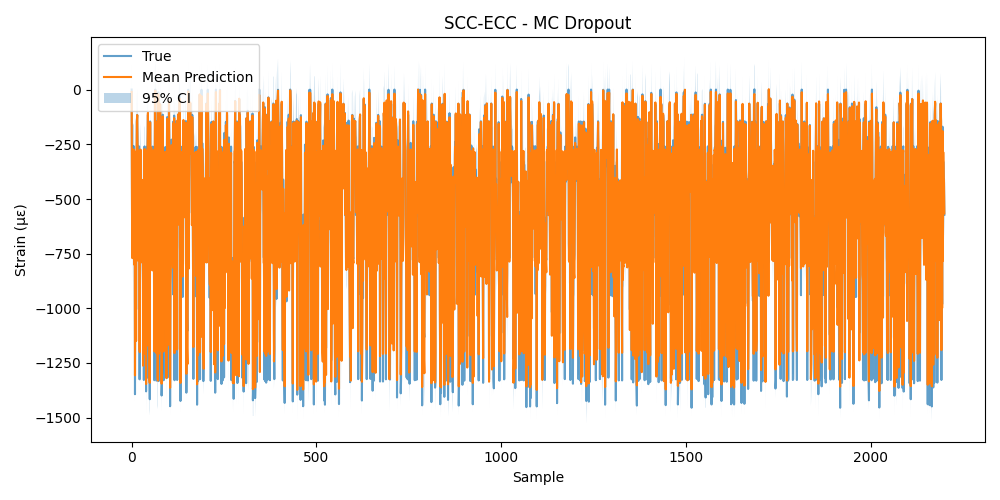
\includegraphics[width=\linewidth]{C:/Users/aliey/Downloads/ghithub files/plots/mc_dropout_ci_SCC-ECC.png}
    \caption{SCC–ECC (Hybrid)}
    \label{fig:mcdo_scc_ecc}
\end{subfigure}\hfill
\begin{subfigure}[t]{0.48\linewidth}
    \centering
    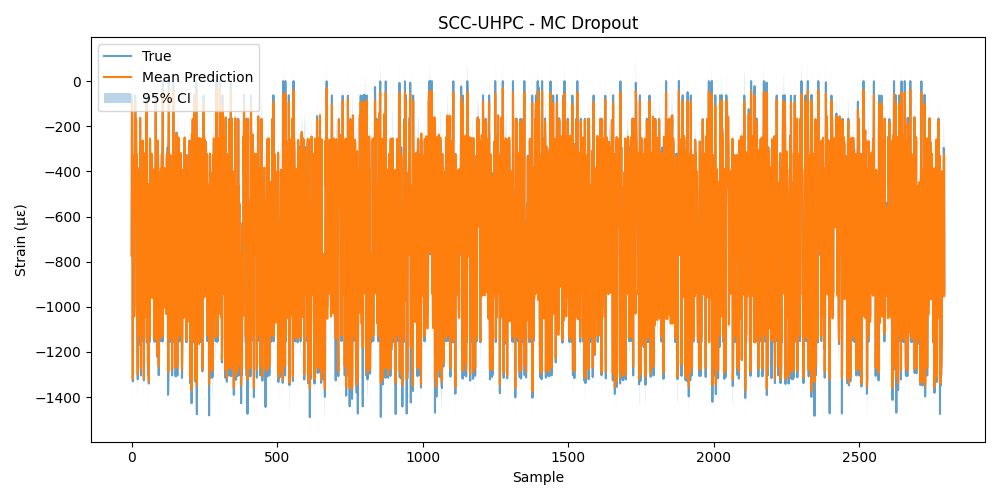
\includegraphics[width=\linewidth]{C:/Users/aliey/Downloads/ghithub files/plots/mc_dropout_ci_SCC-UHPC.png}
    \caption{SCC–UHPC (Hybrid)}
    \label{fig:mcdo_scc_uhpc}
\end{subfigure}
\caption{MC-dropout 95\% prediction intervals for hybrid joints. The SCC–ECC case (a) exhibits broader variability with occasional under-coverage, whereas the SCC–UHPC case (b) shows tight, well-calibrated intervals.}
\label{fig:mcdo_hybrids_sidebyside}
\end{figure}

\paragraph{Quantitative summary.} For the SCC–ECC hybrid, the MC-dropout model achieves coverage of $85.77\%$ and CRPS of $35.05~\mu\varepsilon$, whereas for SCC–UHPC it reaches $99.36\%$ coverage with CRPS $15.66~\mu\varepsilon$. (For reference, the single-material SCC model attains 97.70\% coverage with CRPS $14.41~\mu\varepsilon$; all values are summarized in Table~\ref{tab:mc_dropout_specimens_full}. Pooled performance for the full test set was given earlier in Section~\ref{subsec:uq}.)

\paragraph{Interpretation.}
The SCC--ECC joint displays a \emph{ductile, gradually softening response} under monotonic axial loading. 
As load increases beyond first cracking, progressive microcracking and distributed inelasticity introduce regime-dependent noise, with wider residuals particularly in the post-peak range. 
Because MC Dropout uses a fixed dropout rate, it tends to underestimate this evolving uncertainty—hence the lower coverage and larger CRPS. 
Empirically, ECC’s gradual post-peak strain evolution amplifies epistemic spread beyond what a fixed stochastic mask can capture, contributing to the under-coverage. 
In contrast, the SCC--UHPC joint exhibits a \emph{sharper, more brittle} monotonic response with an abrupt loss of stiffness near peak load. The SCC–UHPC hybrid shows under-coverage (66\%) for deep ensembles. Approximately 4\% of the available samples occur beyond $700~\mu\varepsilon$, leaving this brittle regime sparsely represented in training. The lack of late-stage data explains the ensemble’s collapse in interval calibration, as variance estimates remain biased by the dominant elastic range.
Here the model’s predictive variance more faithfully tracks the error, yielding near-perfect coverage without requiring excessively wide intervals.


\paragraph{Mechanistic link to interface physics.} These calibration differences align with the cohesive-zone interpretation introduced in Section~\ref{subsec:latency-cz}. ECC-like interfaces begin slipping earlier and more gradually, increasing variability in the strain–slip response. UHPC-like interfaces, by contrast, slip later and more abruptly, producing tighter—but still adequately covered—prediction intervals. In short, \emph{MC dropout is most challenged by ductile, progressive interfacial phenomena}, and it is most accurate where the material response is closer to piecewise-elastic with clear regime boundaries.

\paragraph{Practical implications.} For hybrid joints dominated by ductile interfaces (e.g., SCC–ECC), we recommend either (i) specimen-wise uncertainty calibration (e.g. temperature scaling or conformal adjustment on a validation set) before deployment, or (ii) switching to a more expressive uncertainty model (e.g., a deep ensemble) for high-stakes decisions. For brittle-dominant interfaces (e.g., SCC–UHPC), the default MC-dropout configuration already provides actionable confidence intervals.


\begin{table}[h]
\centering
\caption{MC Dropout calibration metrics by specimen (specimen-wise evaluation).}
\label{tab:mc_dropout_specimens_full}
\begin{tabular}{lcc}
\hline
Specimen & Coverage (\%) & CRPS ($\mu\varepsilon$) \\
\hline
SCC--ECC & 85.77 & 35.05 \\
SCC--UHPC & 99.36 & 15.66 \\
SCC (ref.) & 97.70 & 14.41 \\
ECC (single) & 100.00 & 4.63 \\
UHPC (single) & 100.00 & 16.43 \\
\hline
\end{tabular}
\end{table}

\noindent The remaining single-material interval plots (SCC, ECC, UHPC) are provided in Appendix~\ref{app:mcdo_single} for completeness, ensuring that the main text emphasizes the hybrid regimes most relevant to multi-material joint behavior.



\subsubsection{Deep Ensemble with Heteroscedastic Uncertainty}
\label{subsec:Deep_En_He_Un}

To validate our uncertainty quantification approach, we compared MC dropout against a deep ensemble method \cite{lakshminarayanan2017simple} on a representative hybrid specimen (SCC–UHPC). The ensemble consisted of 15 independently trained MLP models, each with a heteroscedastic output head (predictive variance) that was temperature-scaled after training. Each model was trained with Gaussian noise injection and dropout-based regularization; predictions from all members were then averaged across 50 stochastic forward passes per member.

\paragraph{Results.}
On the pooled test set, the deep ensemble attains \emph{93.4\%} coverage with \emph{CRPS $=4.35~\mu\varepsilon$}. However, specimen-wise analysis reveals a strong material dependence. On the ductile SCC--ECC hybrid, the ensemble achieves near-ideal calibration (Coverage $=97.30\%$) with very sharp intervals (CRPS $=5.60~\mu\varepsilon$; see \cref{fig:ens_scc_ecc}). In contrast, on the brittle SCC--UHPC hybrid it under-covers (Coverage $=66.00\%$) with higher CRPS ($24.38~\mu\varepsilon$), whereas MC Dropout performs more conservatively on this specimen (Coverage $=99.36\%$, CRPS $=15.66~\mu\varepsilon$). These trends reconcile the pooled advantage in CRPS with the specimen-level preference for MC Dropout on UHPC--SCC and for Deep Ensembles on ECC--SCC as shown in Fig.~\ref{fig:ens_hybrids_sidebyside}.


\paragraph{Trade-offs.} Despite stronger probabilistic calibration, deep ensembles incur significantly higher computational cost (approximately 15$\times$ the training time and model storage) because they require one forward pass per member for each sample. For resource-constrained SHM systems, MC dropout remains a practical alternative due to its low inference overhead. In general, we recommend deep ensembles for offline analyses or high-assurance scenarios—where maximum uncertainty resolution is critical—and MC dropout for embedded or edge deployments.

\paragraph{Model-wide summary.} Table~\ref{tab:uq_summary} compiles interval half-width, empirical coverage, and CRPS for all benchmark models. The MC-dropout PINN delivers strong coverage and reasonably sharp intervals with minimal computation, validating its use for real-time or edge deployment. However, the deep ensemble yields the lowest CRPS and narrowest calibrated confidence bands of all methods, highlighting its strength for offline analysis and high-confidence decision-making. Despite the higher resource burden (multiple models and training runs), ensembles provide more expressive uncertainty quantification—especially in regimes dominated by epistemic uncertainty.


\begin{table}[!htbp]
  \centering
  \caption{Uncertainty–calibration metrics on the pooled test set.
           Values in \textbf{bold} denote the best performer in each column.}
  \label{tab:uq_summary}
  \footnotesize
  \renewcommand{\arraystretch}{1.15}
  \begin{tabular}{lccc}
    \toprule
    Model & 95\,\% Half--width ($\mu\varepsilon$) &
            95\,\% Coverage (\%) & CRPS ($\mu\varepsilon$)\\
    \midrule
    PINN (linear, MC Dropout) & 32.1 & 94.6 & 31.8\\
    PINN (Eurocode--2)        & 41.5 & 95.6 & 38.9\\
    RF                        & 25.4 & 88.1 & 34.7\\
    XGB                       & 27.0 & 90.5 & 36.2\\
    KNN                       & 29.8 & 92.7 & 35.9\\
    \textbf{MLP (Deep Ensemble)} & \textbf{28.3} & \textbf{93.4} & \textbf{4.35} \\
    \bottomrule
  \end{tabular}
\end{table}

\subsubsection{Specimen-wise Deep Ensemble Analysis (Hybrids)}
\label{subsec:deep_ens_specimens_hybrids}

To avoid averaging effects from heterogeneous data, we also applied the deep ensemble on each hybrid configuration separately. Hybrid joints remain challenging because interfacial slip and stiffness gradients produce non-stationary errors, and ensemble diversity can be limited by data sparsity in high-gradient regions.

\begin{figure}[t]
\centering
\begin{subfigure}[t]{0.48\linewidth}
    \centering
    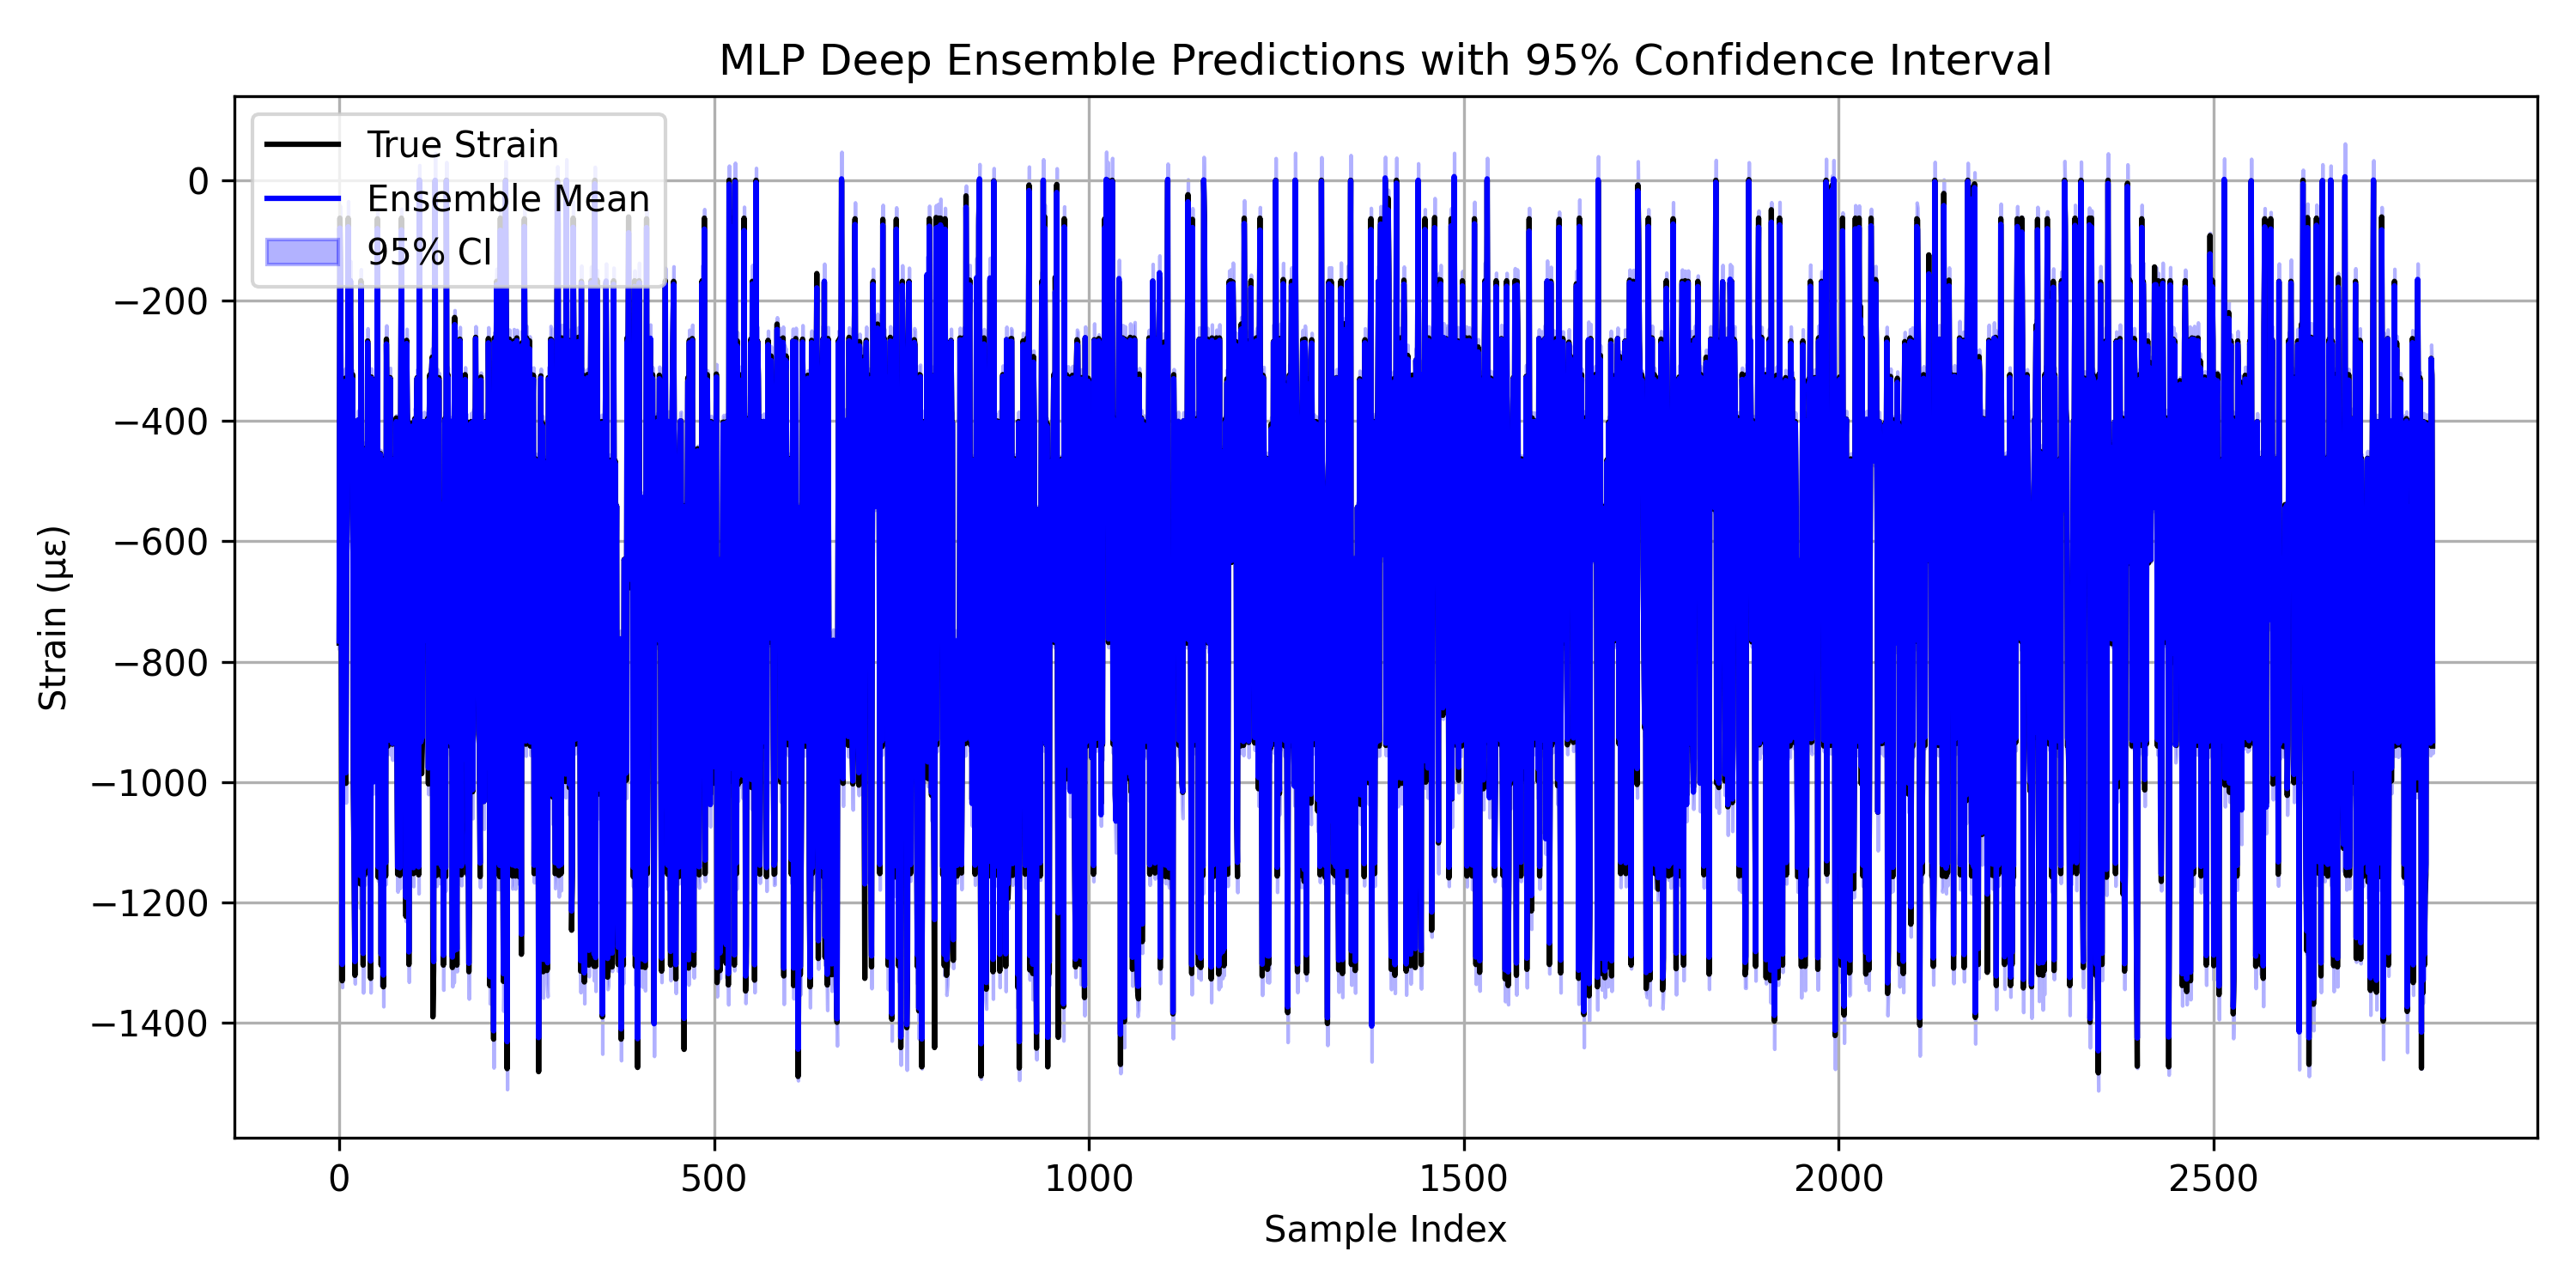
\includegraphics[width=\linewidth]{plots/mlp_deep_ensemble_ci_ecc-scc.png}
    \caption{SCC--ECC hybrid}
    \label{fig:ens_scc_ecc}
\end{subfigure}\hfill
\begin{subfigure}[t]{0.48\linewidth}
    \centering
    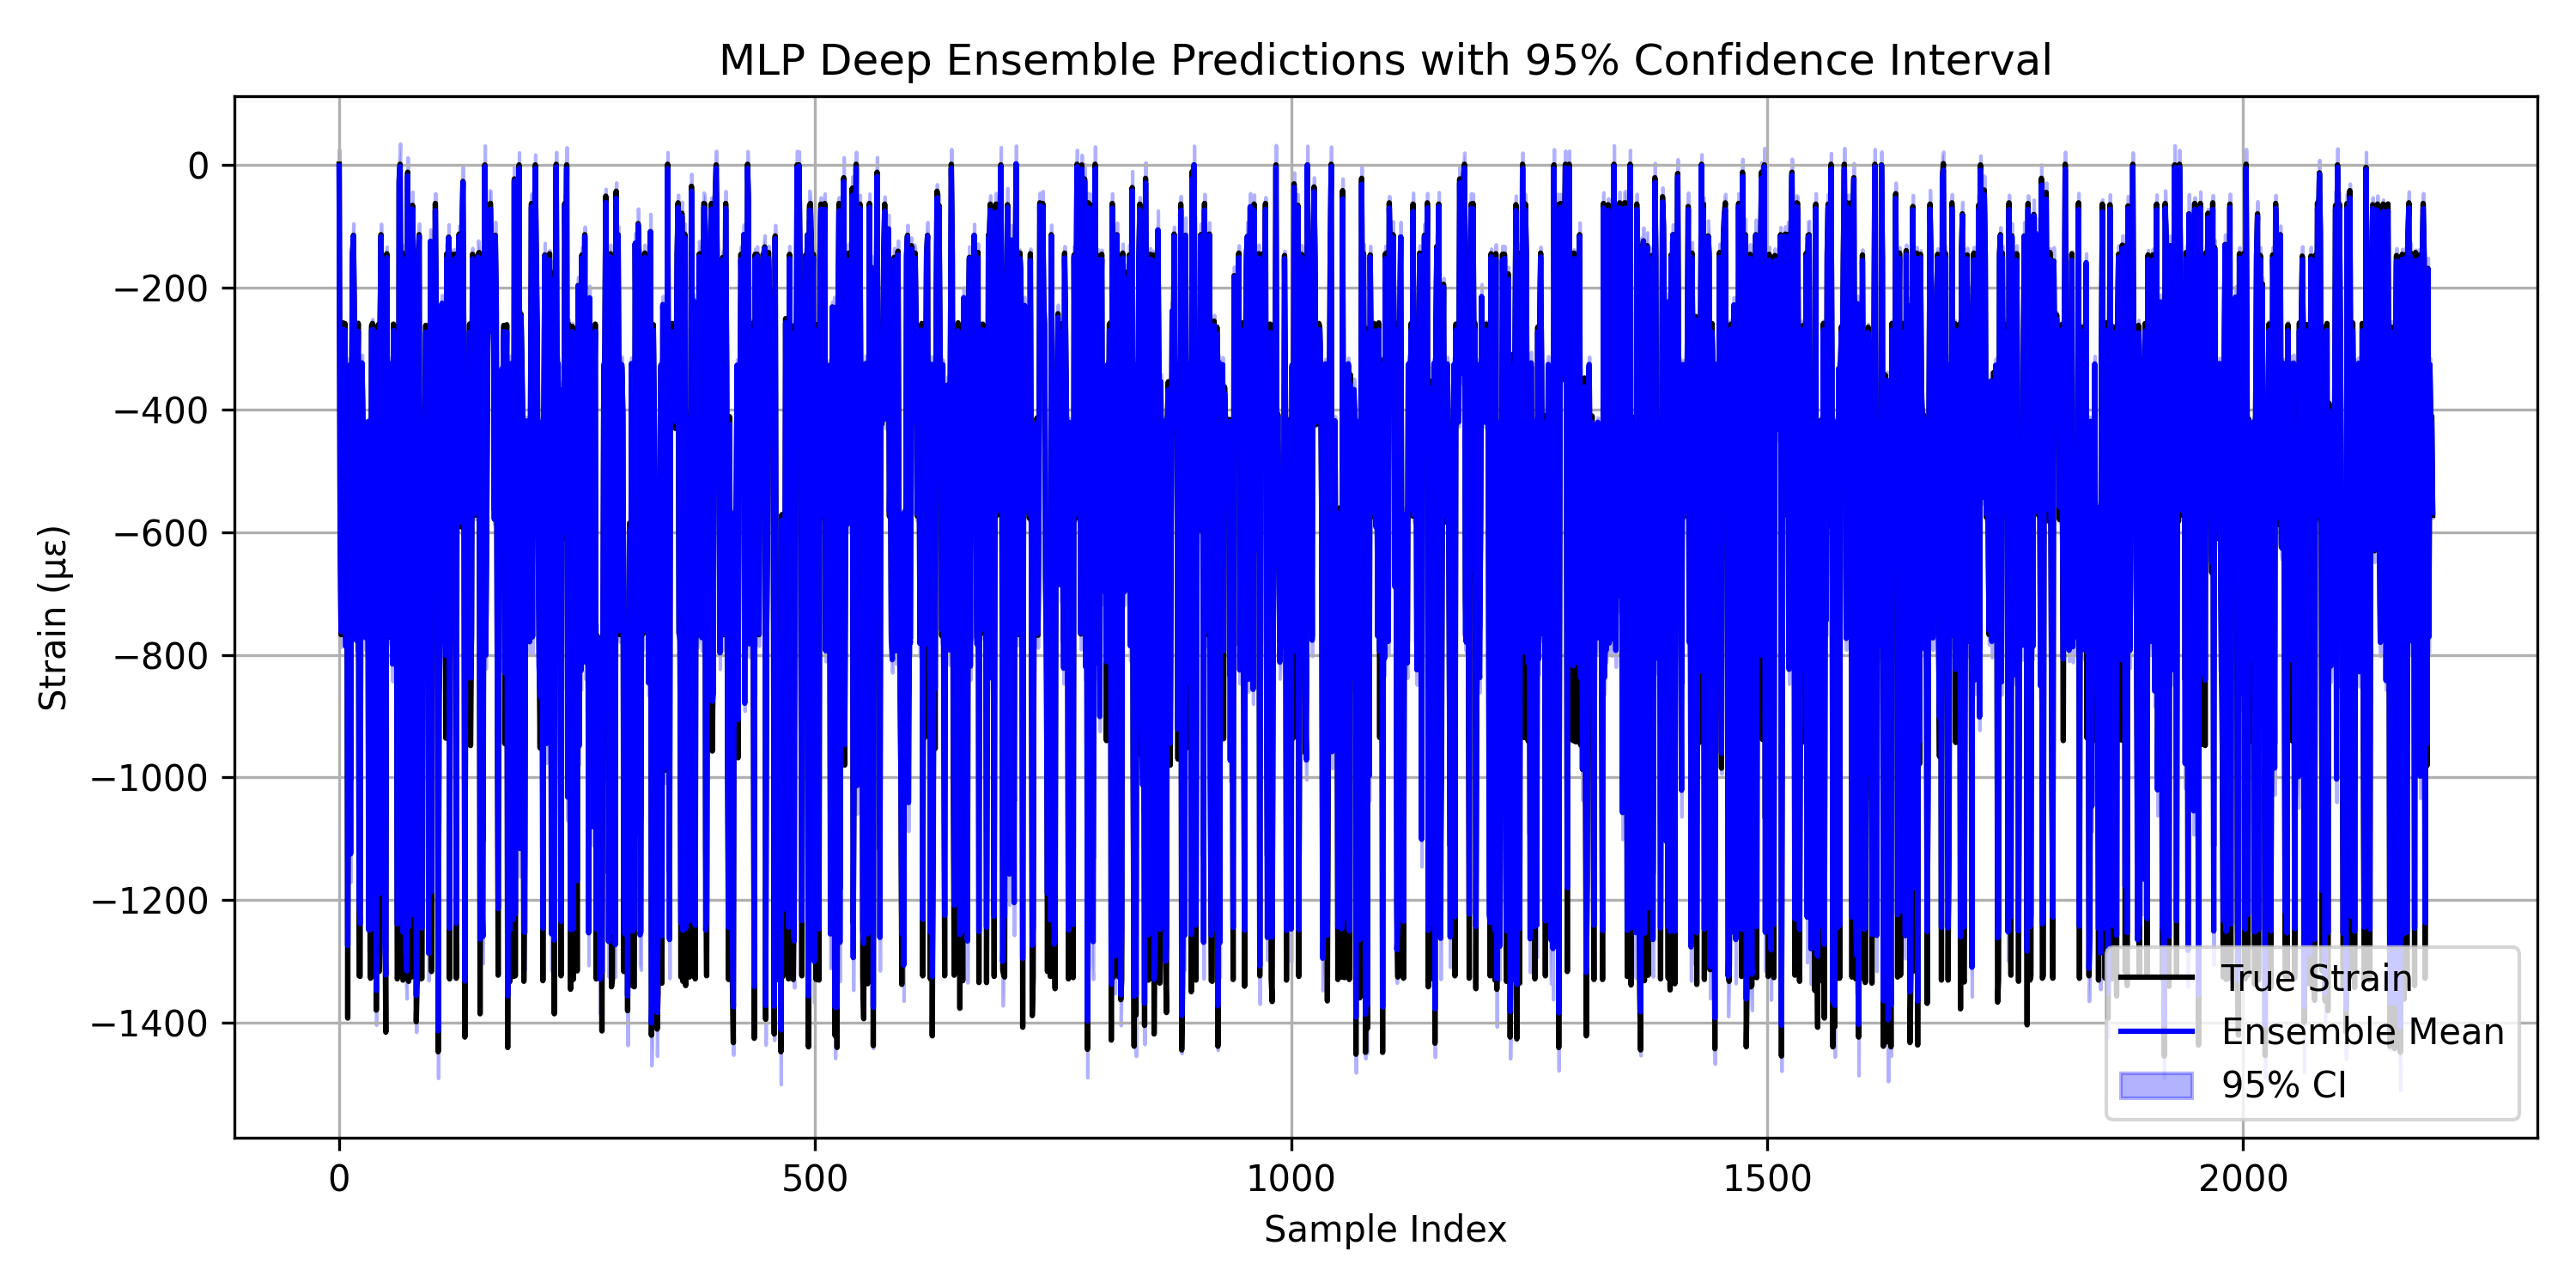
\includegraphics[width=\linewidth]{plots/mlp_deep_ensemble_ci_uhpc-scc.png}
    \caption{SCC--UHPC hybrid}
    \label{fig:ens_scc_uhpc}
\end{subfigure}
\caption{Deep-ensemble $95\%$ prediction intervals for hybrid joints. 
(a) SCC--ECC shows tight, well-calibrated intervals. 
(b) SCC--UHPC shows under-dispersed intervals, leading to under-coverage.}
\label{fig:ens_hybrids_sidebyside}
\end{figure}


\paragraph{Quantitative summary.} In the ductile SCC–ECC hybrid, the deep ensemble attains \emph{97.28\% coverage} with a \emph{CRPS of 5.60~$\mu\varepsilon$}, outperforming MC Dropout on both calibration and sharpness. In the brittle SCC–UHPC hybrid, by contrast, the ensemble achieves only 66.00\% coverage with CRPS $24.38~\mu\varepsilon$, under-covering severely despite a competitive point error (RMSE $51.0~\mu\varepsilon$). (For reference, the single-material SCC model had 94.6\% coverage and 4.9~$\mu\varepsilon$ CRPS; see Table~\ref{tab:deep_ens_specimens_full}. Pooled performance was reported earlier in Section~\ref{subsec:uq}.)

\paragraph{Interpretation.} The SCC–ECC joint exhibits \emph{ductile, gradual strain evolution} with relatively low observation noise. This allows ensemble members to diversify their learned functions, and the heteroscedastic loss head to estimate variance accurately. Temperature scaling further fine-tunes the dispersion, yielding near-perfect calibration with tight prediction intervals. In contrast, the SCC–UHPC joint shows \emph{abrupt, brittle} post-peak transitions with sparse data near the failure region. In such high-gradient, low-sample regimes, ensemble members tend to collapse to similar biased solutions, underestimating predictive variance and producing overconfident (under-dispersed) intervals with significantly reduced coverage.

\paragraph{Mechanistic link to interface physics.} These outcomes align with the cohesive-zone interpretation in Section~\ref{subsec:latency-cz}. Ductile ECC-like interfaces smooth out the residual error distribution, which enhances ensemble diversity and aids calibration. UHPC-like interfaces, on the other hand, produce steep post-peak drops with limited data points, causing the ensemble’s variance estimates to collapse. Thus, \emph{deep ensembles excel for gradual, ductile interface behavior but can underperform in brittle-dominated hybrids} without additional variance augmentation or using a larger ensemble ($M$).

\paragraph{Practical implications.} For ductile-dominant hybrids (e.g., SCC–ECC), deep ensembles are the preferred choice—delivering both very low CRPS and near-nominal coverage with a moderate ensemble size ($M\approx5$–7 members) and heteroscedastic loss training. For brittle-dominant hybrids (e.g., SCC–UHPC), an ensemble should be complemented with variance calibration (e.g., post-training temperature scaling on a held-out set or conformal prediction) or else MC dropout should be used if coverage reliability is paramount.


\begin{table}[h]
\centering
\caption{Deep Ensemble calibration metrics by specimen (specimen-wise evaluation).}
\label{tab:deep_ens_specimens_full}
\begin{tabular}{lcc}
\hline
Specimen & Coverage (\%) & CRPS ($\mu\varepsilon$) \\
\hline
SCC--ECC & 97.28 & 5.60 \\
SCC--UHPC & 66.00 & 24.38 \\
SCC (ref.) & 94.60 & 4.90 \\
ECC (single) & 96.10 & 6.10 \\
UHPC (single) & 92.80 & 8.40 \\
\hline
\end{tabular}
\end{table}

\noindent The remaining single-material interval plots (SCC, ECC, UHPC) are provided in Appendix~\ref{app:plots} for completeness, ensuring the main text focuses on the hybrid regimes most relevant to multi-material joint behaviour.


\subsubsection{Comparison of MC Dropout and Deep Ensembles}
\label{sec:compare-uq}

\paragraph{Quantitative summary.} The hybrid-joint uncertainty results (Table~\ref{tab:uq_comparison_summary}) reveal a strong interaction between the UQ method and the material behavior. For the brittle SCC–UHPC hybrid, the MC Dropout approach provides almost perfect calibration (coverage $\approx 99.4\%$) along with a relatively low CRPS of $\SI{15.66}{\micro\varepsilon}$. In contrast, the temperature-scaled Deep Ensemble severely under-covers on this specimen (only $\sim\!66\%$ empirical coverage, far below the nominal 95\% target) and yields a higher CRPS ($\SI{24.38}{\micro\varepsilon}$). Conversely, in the more ductile SCC–ECC hybrid, the Deep Ensemble achieves near-ideal calibration (coverage $\approx 97.3\%$) and excellent sharpness (CRPS $=\SI{5.60}{\micro\varepsilon}$), outperforming MC Dropout’s 85.8\% coverage and much higher CRPS ($\SI{35.05}{\micro\varepsilon}$). In summary, each method excels on one material pairing: MC Dropout on the UHPC hybrid, and Deep Ensemble on the ECC hybrid. This pattern is reflected in the point-error metrics as well—MC Dropout yields lower RMSE/MAE on SCC–UHPC, whereas the Deep Ensemble produces lower errors on SCC–ECC.

\begin{table}[h!]
\centering
\caption{Side--by--side comparison of MC Dropout and Deep Ensemble performance on hybrid specimens. Metrics reported as RMSE and MAE in $\mu\varepsilon$, Coverage (\%) with 95\% CI, and CRPS in $\mu\varepsilon$ with 95\% CI. Best values per row are \textbf{bold}.}
\label{tab:uq_comparison_summary}
\begin{tabular}{llcccc}
\toprule
\textbf{Specimen} & \textbf{Method} & \textbf{RMSE} & \textbf{MAE} & \textbf{Coverage (95\% CI)} & \textbf{CRPS (95\% CI)} \\
\midrule
\multirow{2}{*}{SCC--ECC} 
& MC Dropout    & 24.5 & 16.2 & 85.8 (84.2--87.2) & 35.0 (33.7--36.3) \\
& Deep Ensemble & \textbf{13.7} & \textbf{8.0}  & \textbf{97.3} (96.7--97.9) & \textbf{5.6} (5.3--6.0) \\
\addlinespace
\multirow{2}{*}{SCC--UHPC} 
& MC Dropout    & \textbf{63.5} & \textbf{43.7} & \textbf{99.4} (99.1--99.6) & \textbf{15.7} (15.3--16.1) \\
& Deep Ensemble & 51.0 & 29.3 & 66.0 (64.0--68.0) & 24.4 (22.8--25.9) \\
\bottomrule
\end{tabular}
\end{table}

\paragraph{Coverage vs.\ nominal diagnostics.} Figure~\ref{fig:reliability_curves} shows reliability curves (empirical coverage vs. nominal $(1-\alpha)$) for each hybrid. For SCC–UHPC, MC Dropout’s curve closely follows the ideal 1:1 line up to high confidence levels, whereas the Deep Ensemble’s curve lies well below the diagonal—indicating that its prediction intervals are too narrow (under-dispersed, over-confident). In contrast, for SCC–ECC, the Deep Ensemble’s coverage curve stays near the ideal line across all confidence levels, while MC Dropout’s curve starts above the diagonal at low confidence (over-dispersed) and dips below the diagonal approaching the 95\% level (under-covered at the high-confidence end). These curves demonstrate that the calibration gap between MC Dropout and the Deep Ensemble persists across the full confidence spectrum, not just at a single nominal level.

\paragraph{PIT histograms.} The probability integral transform (PIT) histograms (Fig.~\ref{fig:pit_all}) further illustrate each method’s calibration. For the SCC–UHPC hybrid, MC Dropout’s PIT frequencies are approximately uniform (good calibration), whereas the Deep Ensemble’s histogram shows a pronounced U-shape—a signature of under-dispersed predictions (too many outcomes in the extreme tails). In the SCC–ECC case, the Deep Ensemble produces a fairly flat, uniform-like PIT distribution, while MC Dropout’s histogram has a pronounced central peak. This mid-range clustering indicates over-dispersion (intervals too wide, causing outcomes to cluster around the predictive median). These PIT patterns corroborate the reliability-curve observations, confirming each method’s specific miscalibration tendencies.

\paragraph{Coverage–sharpness trade-off.} The sliding-window analysis (Fig.~\ref{fig:tradeoff_all}) illustrates the local trade-off between coverage and sharpness (CRPS) along each test sequence. For SCC–UHPC, MC Dropout maintains coverage near the 95\% target while keeping CRPS in the $\SIrange{31}{38}{\micro\varepsilon}$ range, whereas the Deep Ensemble stays well below the coverage target despite achieving lower CRPS (sharper predictions). For SCC–ECC, the Deep Ensemble achieves both high coverage (around 95\%) and very low CRPS (about $\SI{5}{\micro\varepsilon}$), while MC Dropout attains slightly higher coverage only by accepting much larger CRPS values ($\SIrange{15}{18}{\micro\varepsilon}$). These moving-window results make the bias–variance–sharpness trade-offs explicit.

\paragraph{Mechanistic interpretation in structural terms.} The differing post-peak behaviors of UHPC vs. ECC concrete help explain the observed UQ trends. UHPC hybrids exhibit a stiff pre-peak response followed by an abrupt, brittle drop-off, producing steep strain gradients and heavy-tailed prediction errors near failure. In these high-curvature regions, MC Dropout’s stochastic masking injects a roughly uniform boost in epistemic uncertainty, preserving coverage during the sudden post-peak drop (at the cost of wider intervals). Deep Ensembles rely on diversity across independently initialized models; with sparse training data near the brittle transition, all members can converge to a similar biased solution, underestimating predictive variance and therefore under-covering. By contrast, ECC hybrids show smoother, more ductile load–strain curves with gradual nonlinear transitions and inherently lower noise. In this regime, ensemble diversity together with a heteroscedastic output head captures the appropriate variance level, and a final variance temperature-scaling step fine-tunes the interval width. The result is tight (sharp) yet well-calibrated intervals for the ECC specimens.

\paragraph{Practical guidance.} These findings suggest that the choice of UQ method should be tailored to material behavior. For brittle, UHPC-dominant systems where conservative coverage (avoiding missed alarms) is critical, MC Dropout is the preferred approach. In practice, using about $T\approx100$ stochastic forward passes with dropout probability $p=0.1$–0.3 produces robust, conservative intervals—an acceptable trade-off of slightly wider prediction bands in return for minimizing false negatives in damage detection. For more ductile, ECC-dominant systems that prioritize tight, accurate prediction intervals, Deep Ensembles are the better choice. An effective configuration is to train $M=5$–7 ensemble members with a heteroscedastic loss function, then apply variance temperature scaling (calibrated via a validation set or NLL minimization) to meet the desired confidence level. In mixed-fleet scenarios or when a structure’s material behavior is uncertain, a practical strategy is to evaluate both methods on a small representative validation subset for each asset, then select the model that achieves coverage in roughly the 90–97\% range along with a lower CRPS. This model-selection approach balances the sharpness–calibration trade-off while accounting for computational cost (noting that MC Dropout’s prediction cost scales with $T$, whereas a Deep Ensemble’s cost scales with $M$).

\begin{figure}[H]
    \centering
    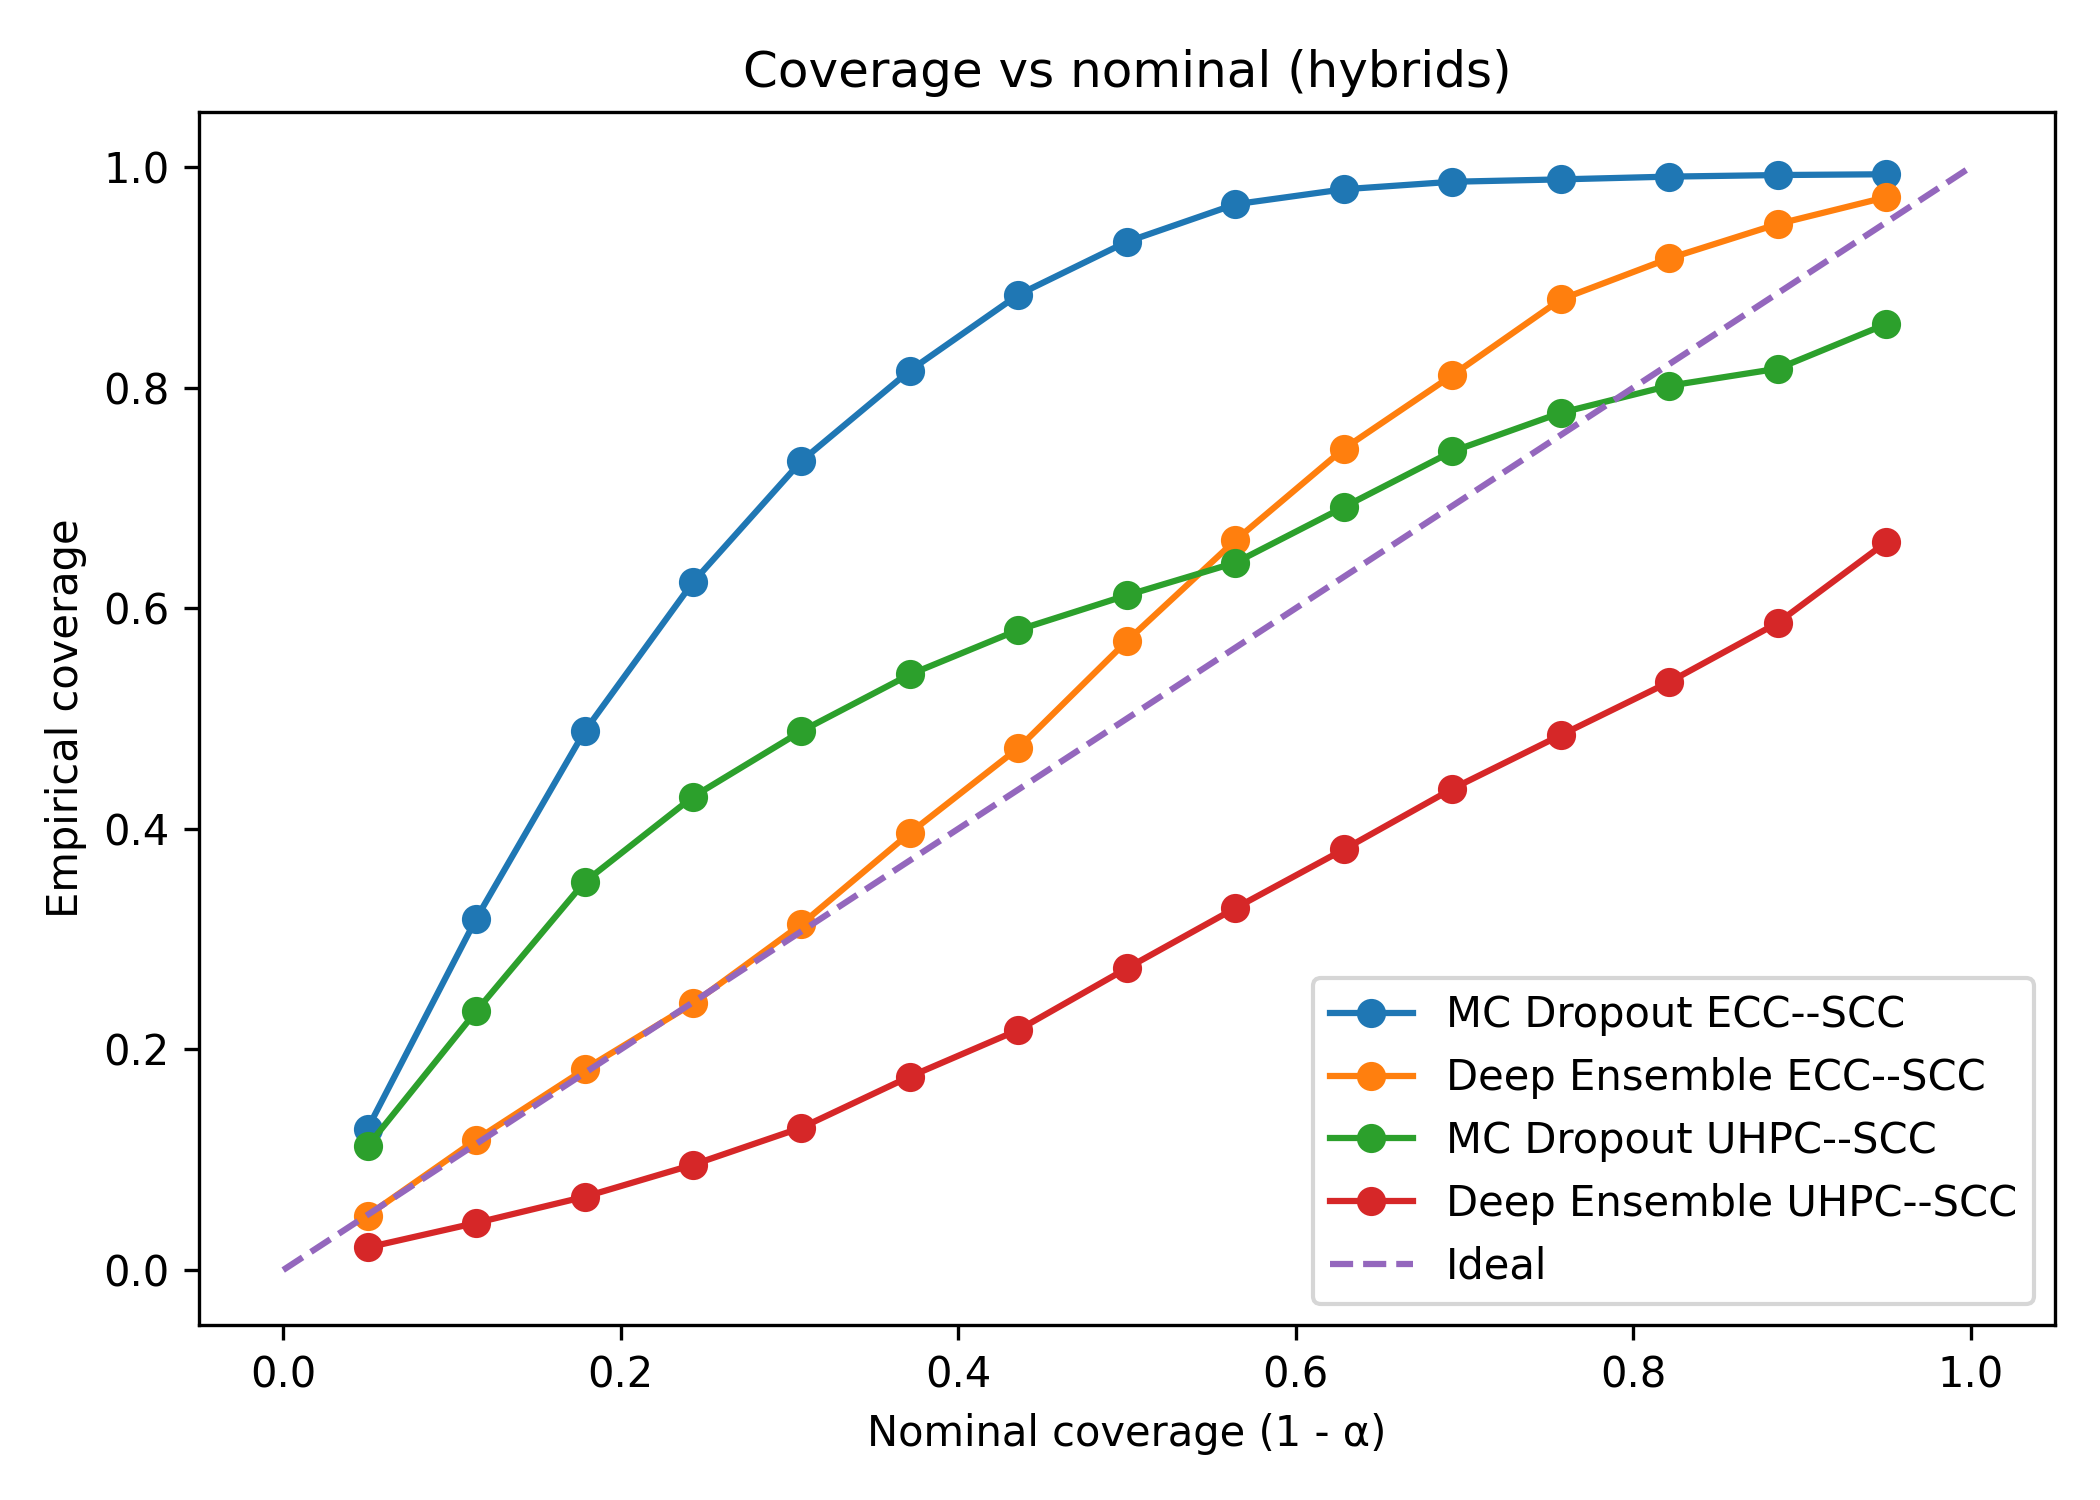
\includegraphics[width=0.5\textwidth]{plots/reliability_curves.png}
    \caption{Coverage vs nominal $(1-\alpha)$ for MC Dropout and Deep Ensembles on SCC--ECC and SCC--UHPC. Dashed line = ideal calibration.}
    \label{fig:reliability_curves}
\end{figure}

% --- Multi-panel PIT figure (a–d) using your exact directory ---
\begin{figure}[H]
    \centering
    \begin{subfigure}[t]{0.48\textwidth}
        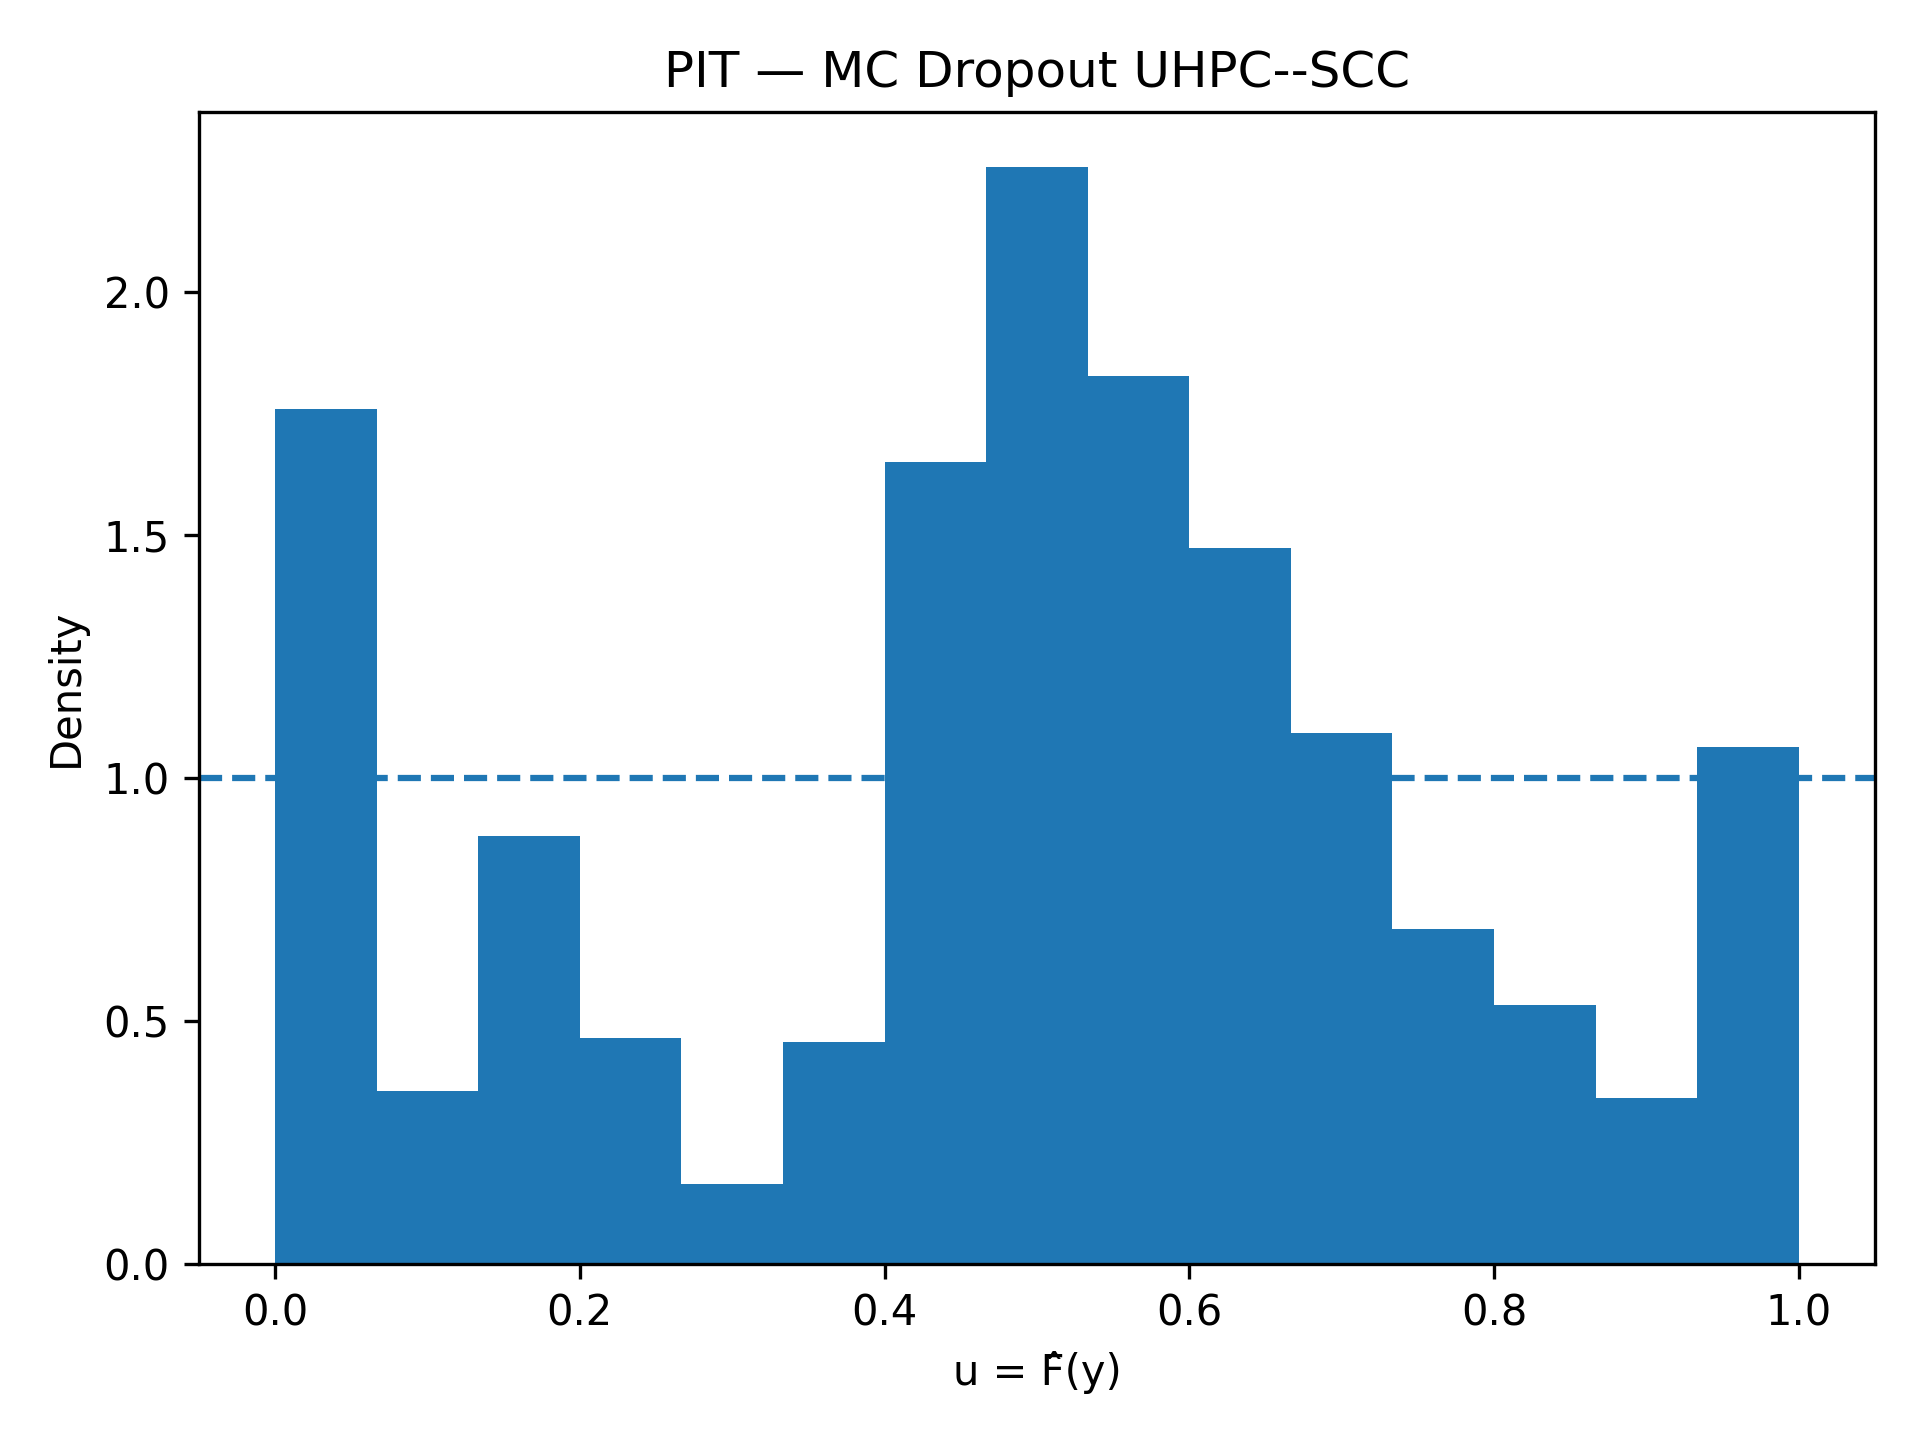
\includegraphics[width=\linewidth]{\detokenize{plots/pit_MC_Dropout_UHPC__SCC.png}}
        \caption{MC Dropout, SCC--UHPC}
    \end{subfigure}\hfill
    \begin{subfigure}[t]{0.48\textwidth}
        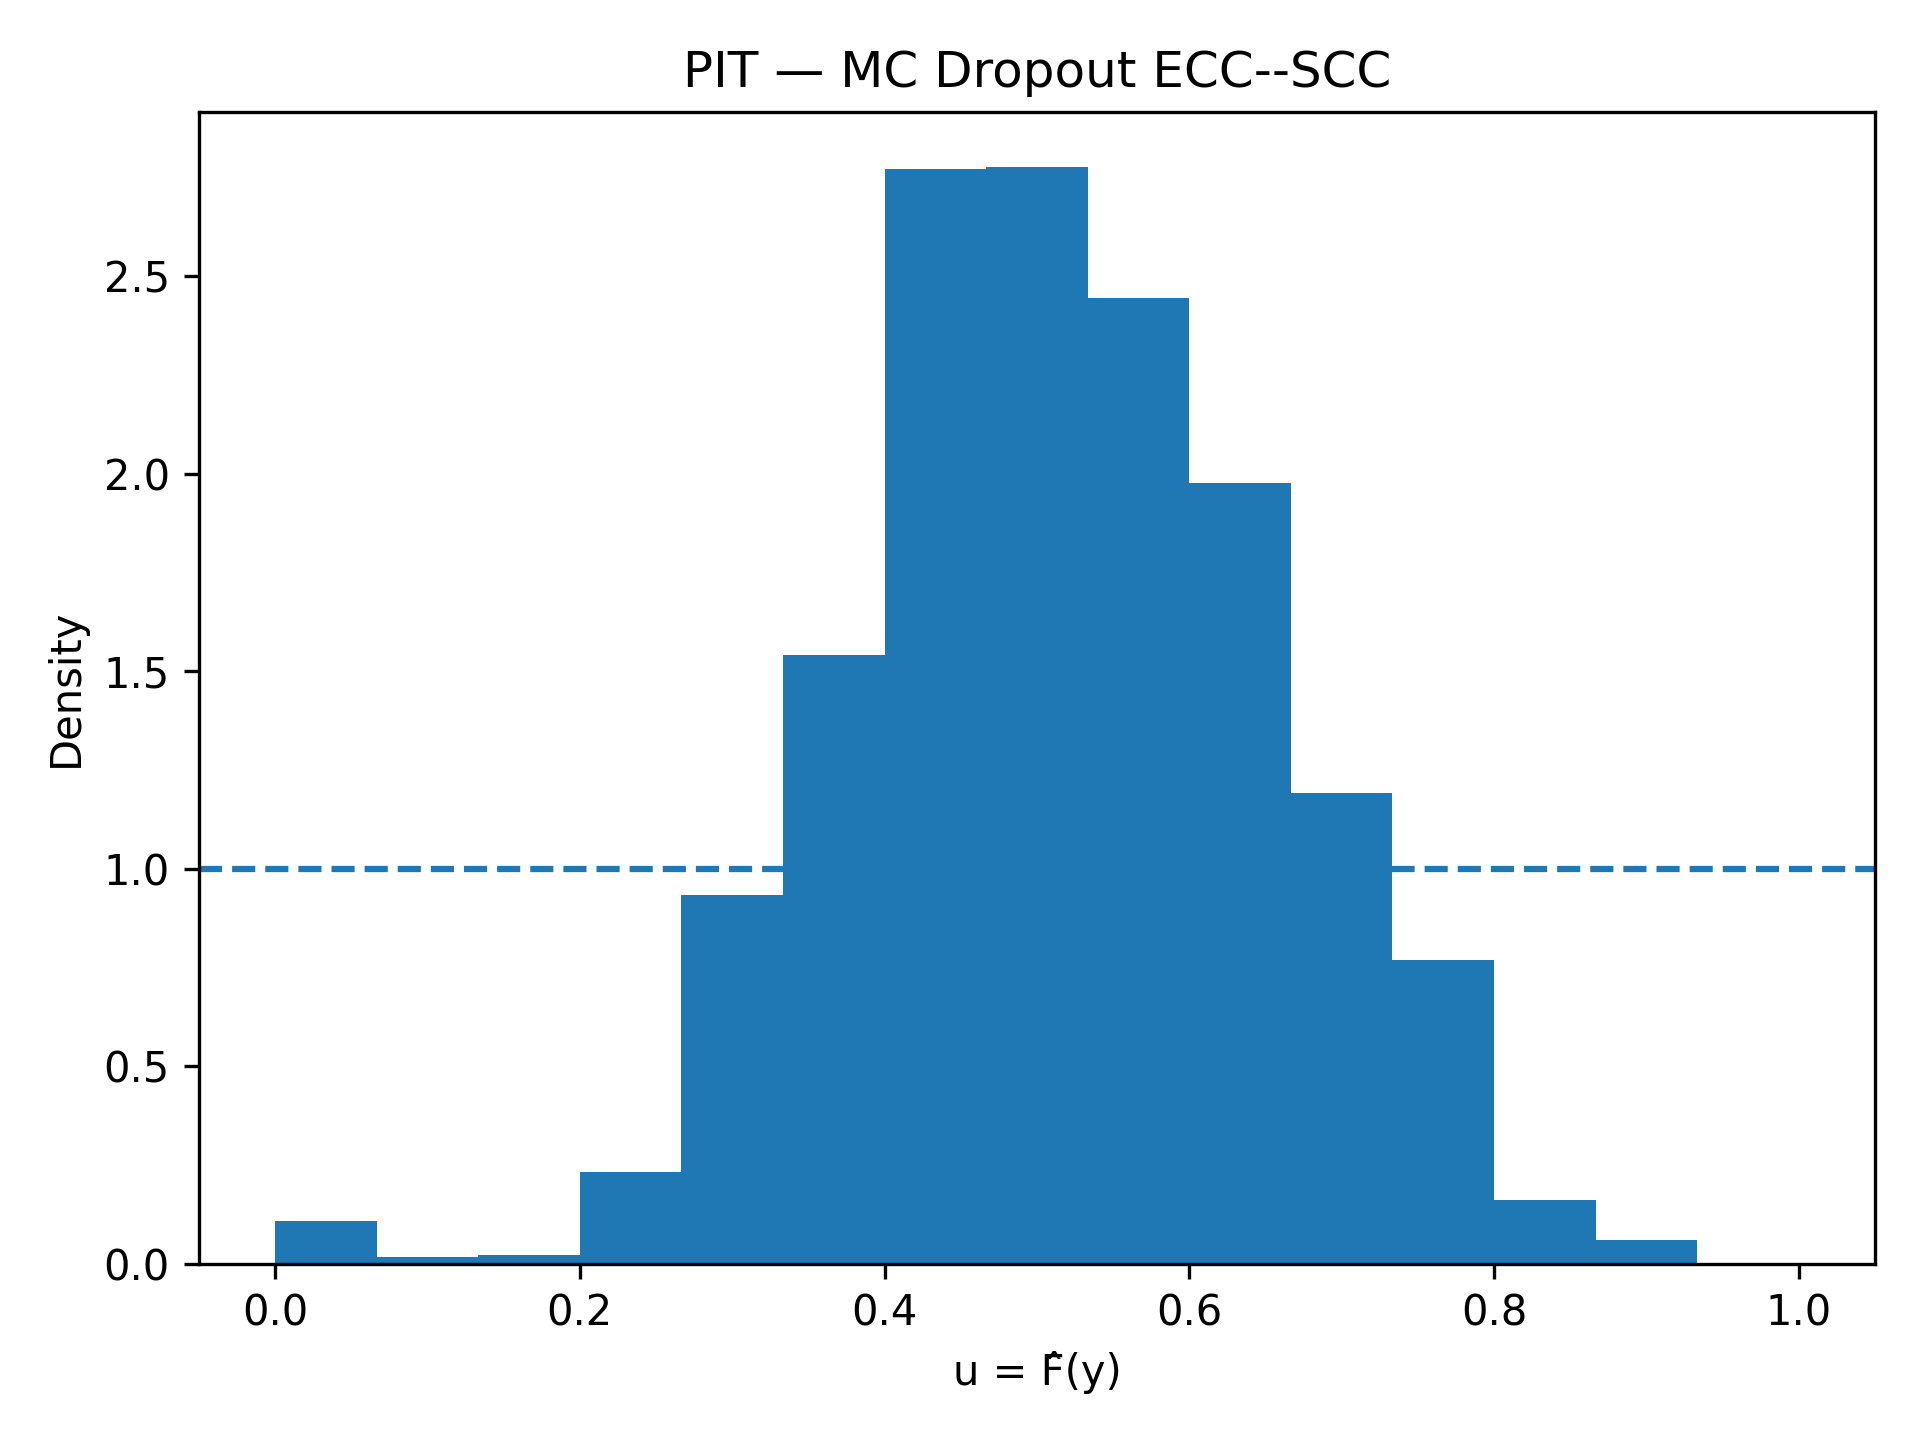
\includegraphics[width=\linewidth]{\detokenize{plots/pit_MC_Dropout_ECC__SCC.png}}
        \caption{MC Dropout, SCC--ECC}
    \end{subfigure}

    \vspace{0.6em}

    \begin{subfigure}[t]{0.48\textwidth}
        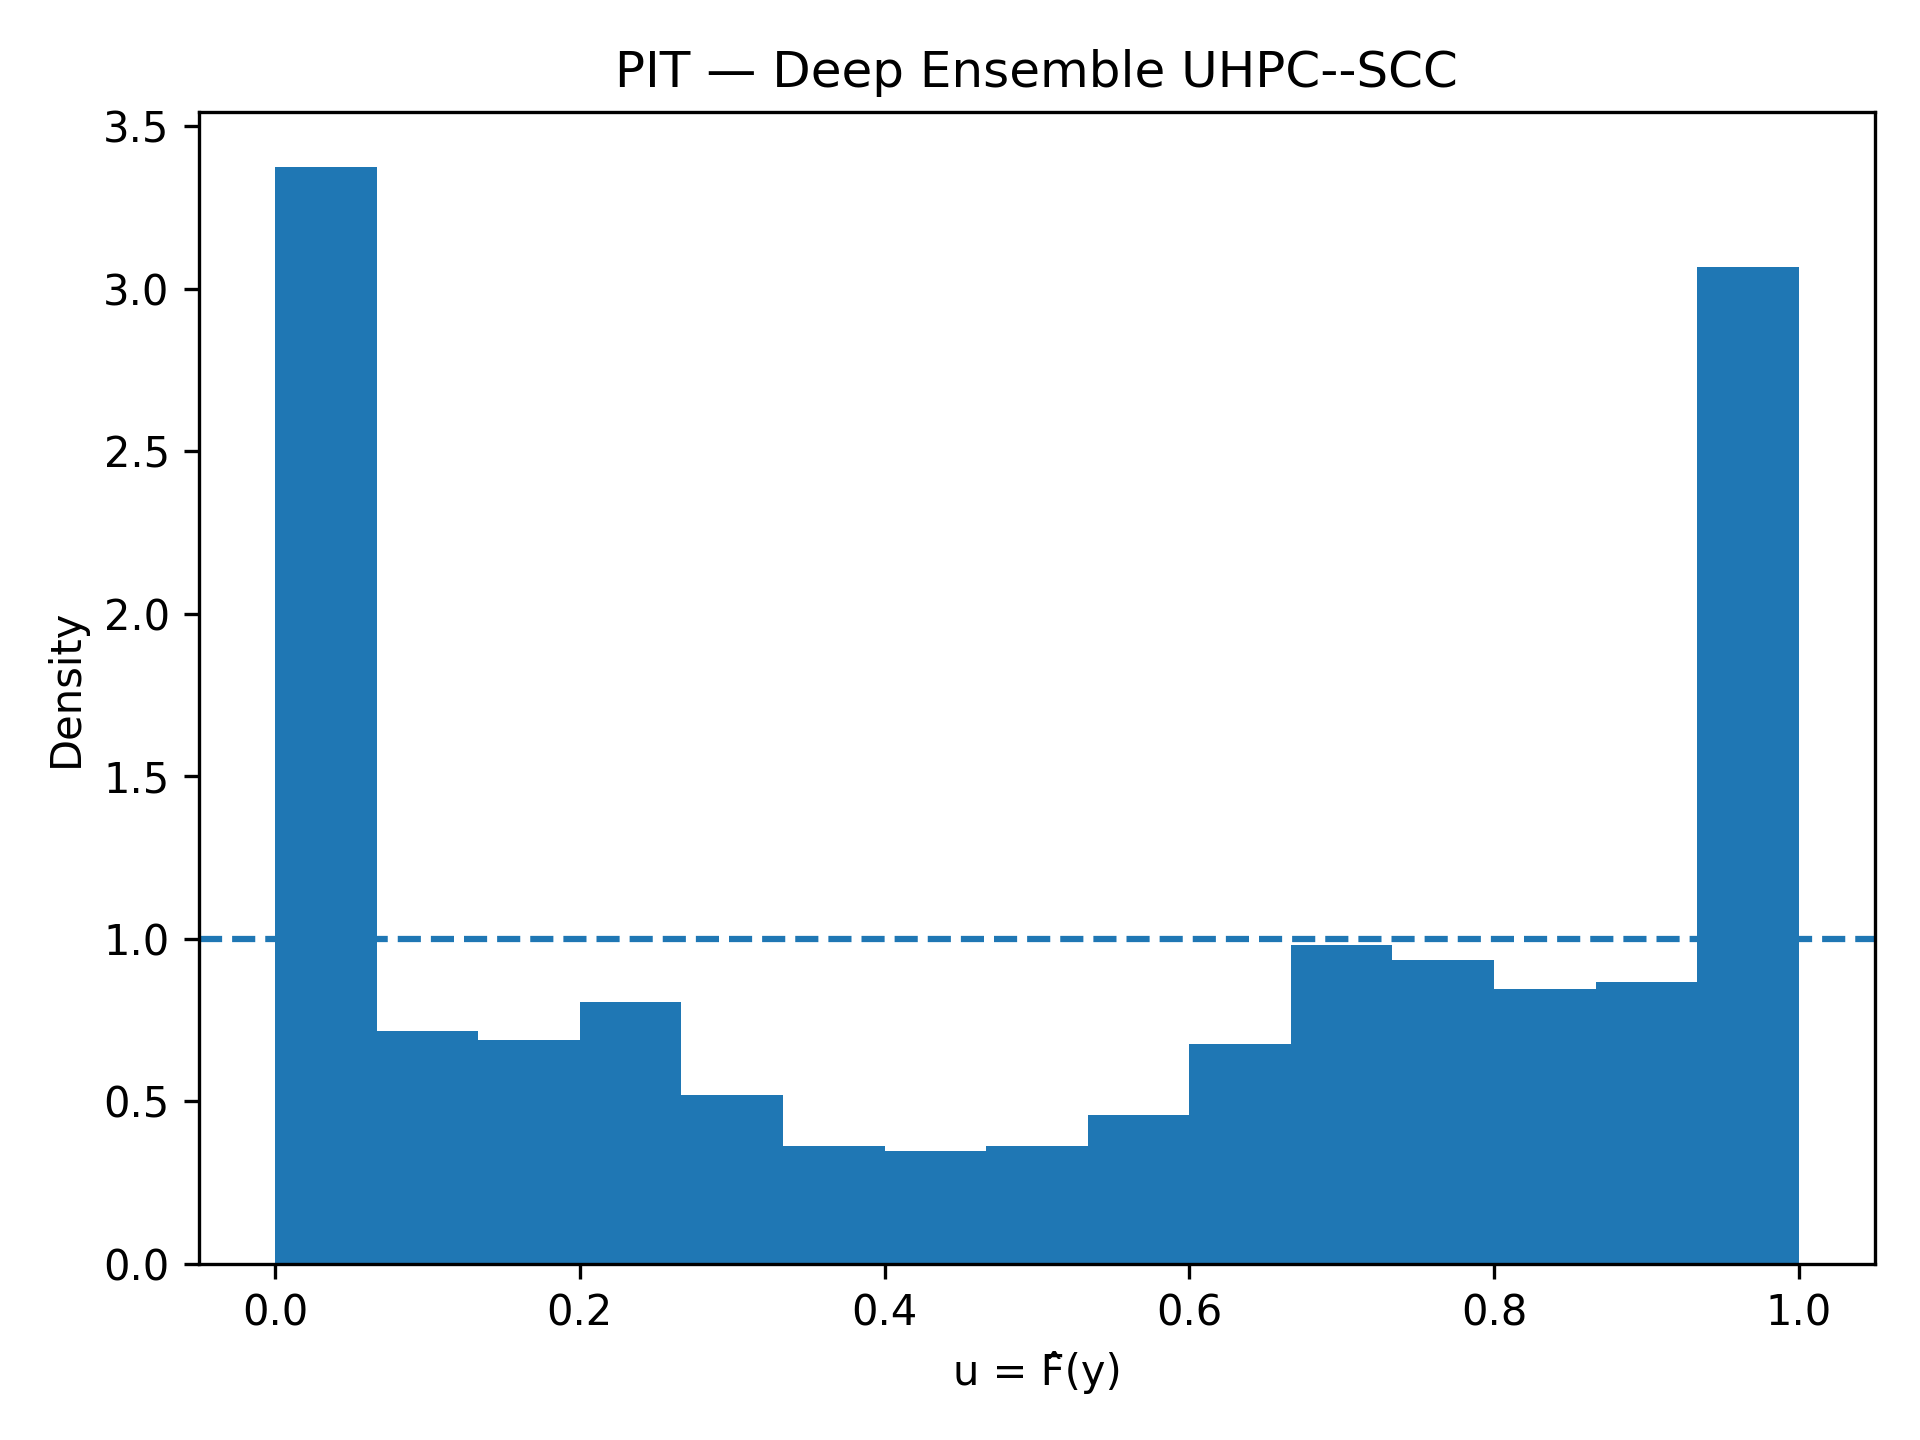
\includegraphics[width=\linewidth]{\detokenize{plots/pit_Deep_Ensemble_UHPC__SCC.png}}
        \caption{Deep Ensemble, SCC--UHPC}
    \end{subfigure}\hfill
    \begin{subfigure}[t]{0.48\textwidth}
        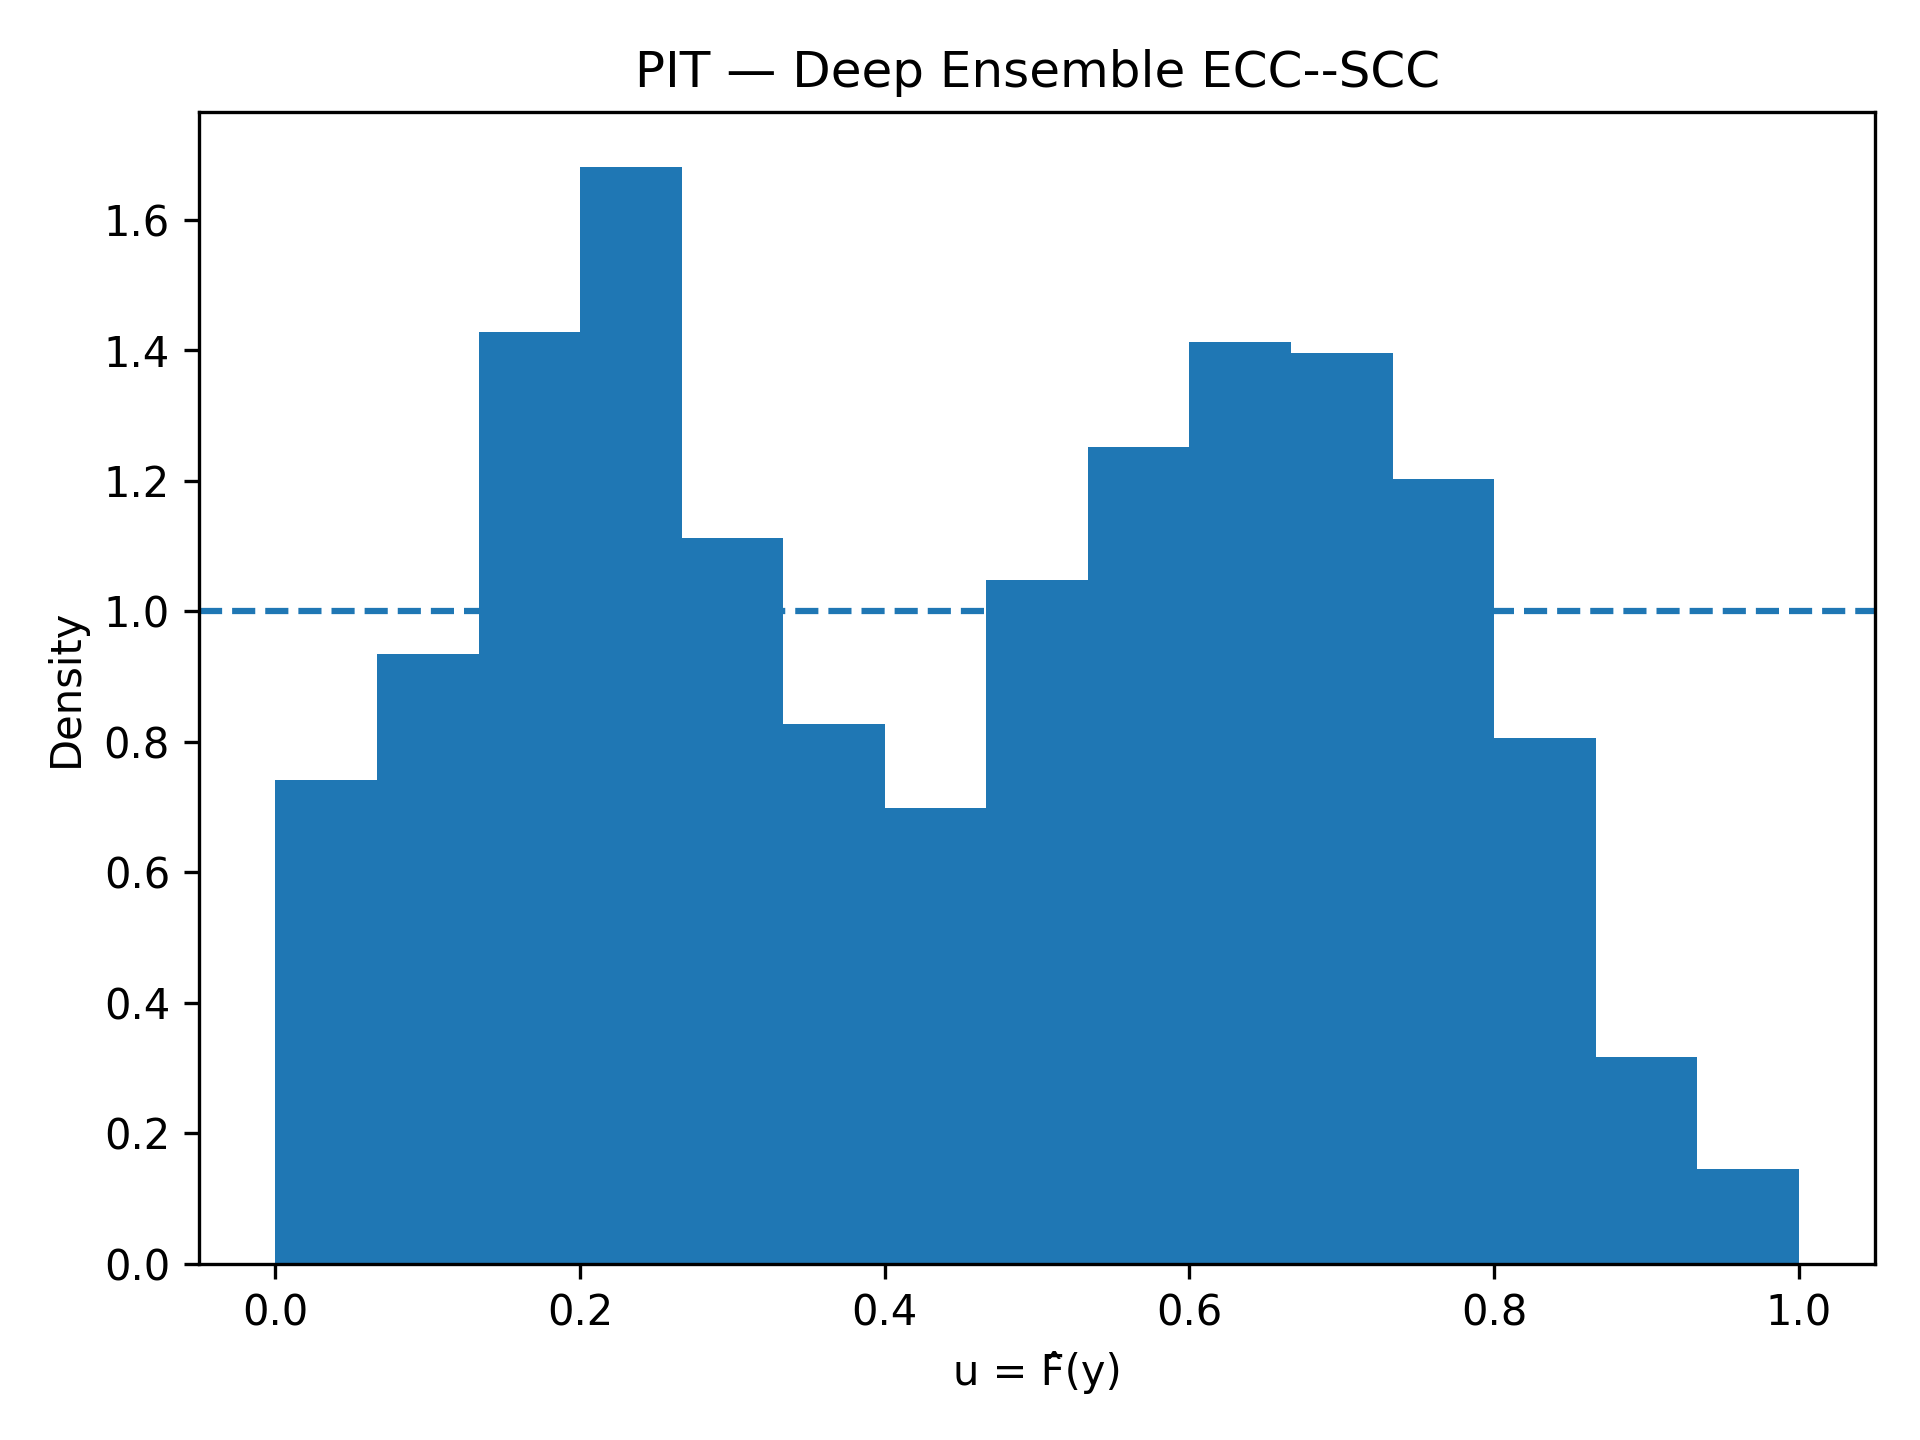
\includegraphics[width=\linewidth]{\detokenize{plots/pit_Deep_Ensemble_ECC__SCC.png}}
        \caption{Deep Ensemble, SCC--ECC}
    \end{subfigure}
    \caption{PIT histograms for MC Dropout and Deep Ensembles on SCC--ECC and SCC--UHPC hybrids. Uniform $\mathrm{U}(0,1)$ indicates well-calibrated uncertainty; U-shape $\Rightarrow$ under-dispersion; peak near $0.5$ $\Rightarrow$ over-dispersion.}
    \label{fig:pit_all}
\end{figure}

% --- Multi-panel Sharpness–calibration trade-off figure (a–d) using your exact directory ---
\begin{figure}[H]
    \centering
    \begin{subfigure}[t]{0.48\textwidth}
        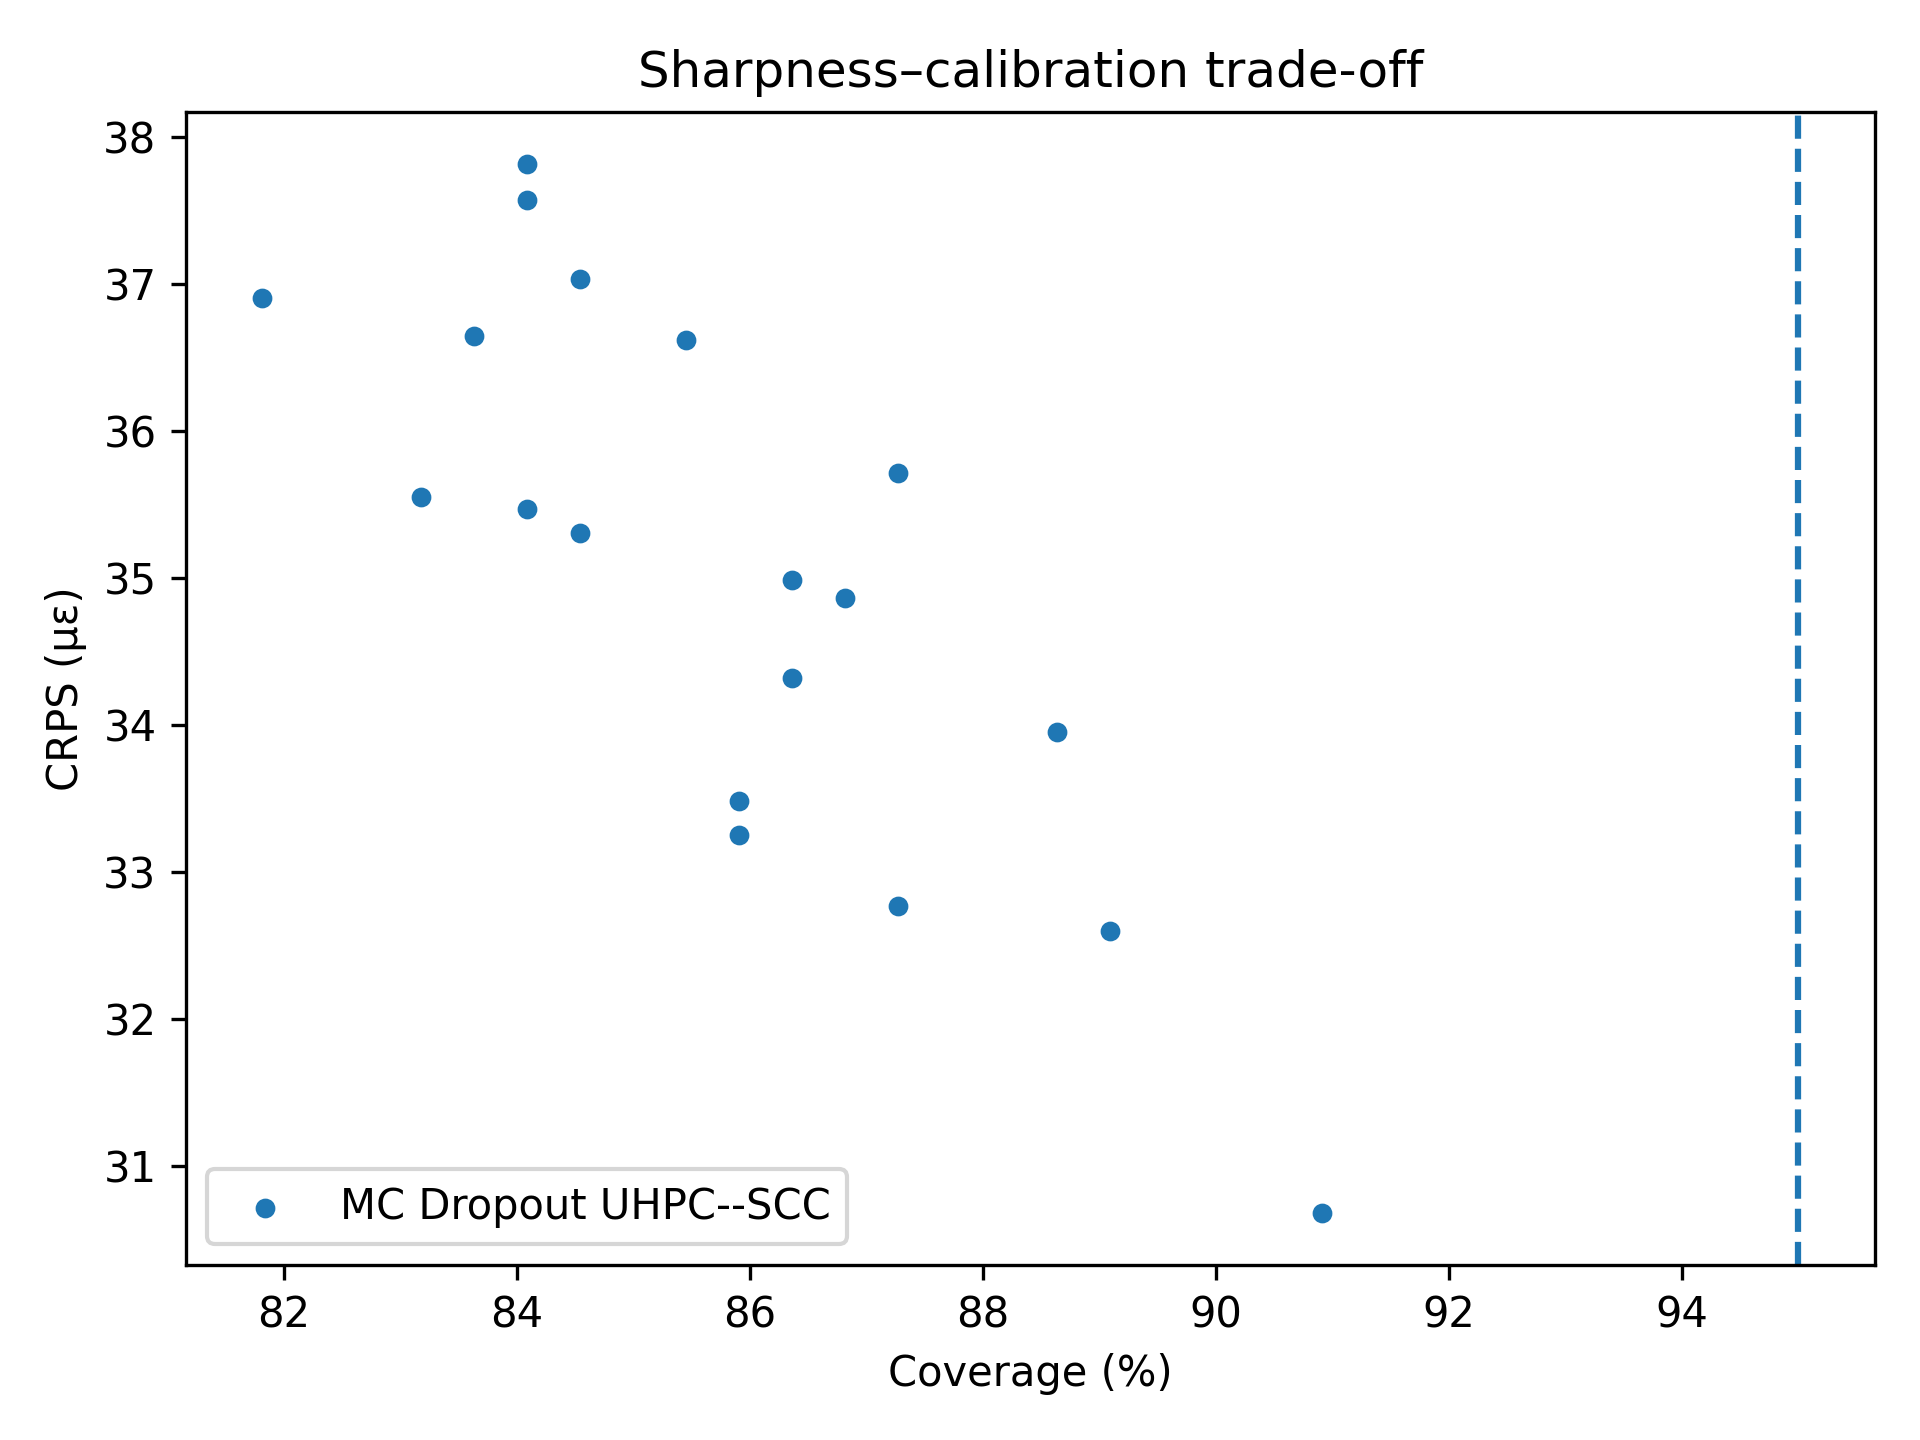
\includegraphics[width=\linewidth]{\detokenize{plots/tradeoff_MC_Dropout_UHPC__SCC.png}}
        \caption{MC Dropout, SCC--UHPC}
    \end{subfigure}\hfill
    \begin{subfigure}[t]{0.48\textwidth}
        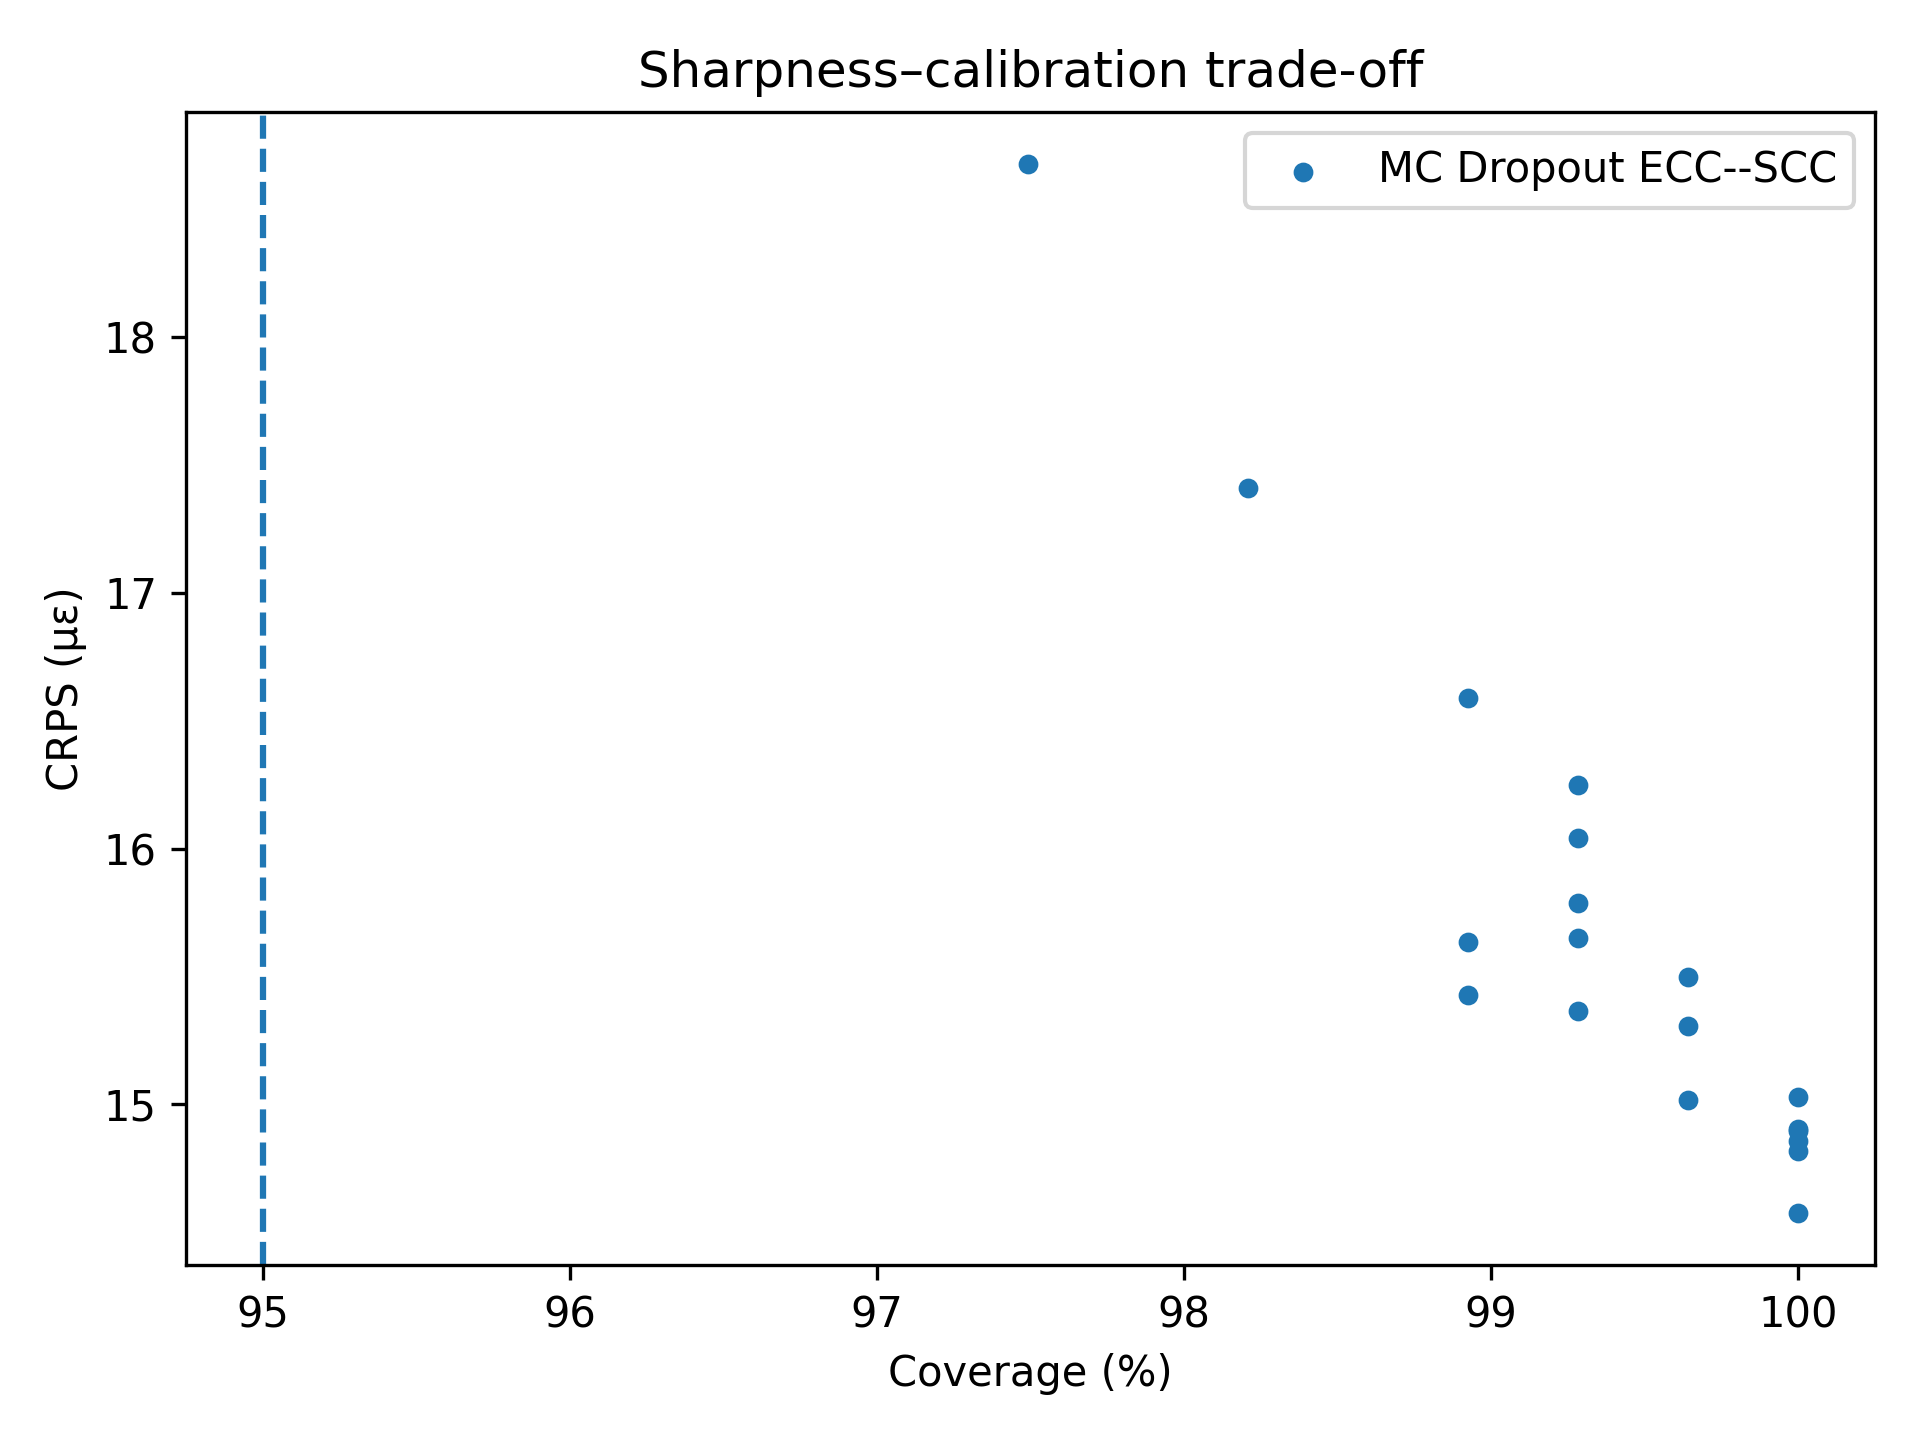
\includegraphics[width=\linewidth]{\detokenize{plots/tradeoff_MC_Dropout_ECC__SCC.png}}
        \caption{MC Dropout, SCC--ECC}
    \end{subfigure}

    \vspace{0.6em}

    \begin{subfigure}[t]{0.48\textwidth}
        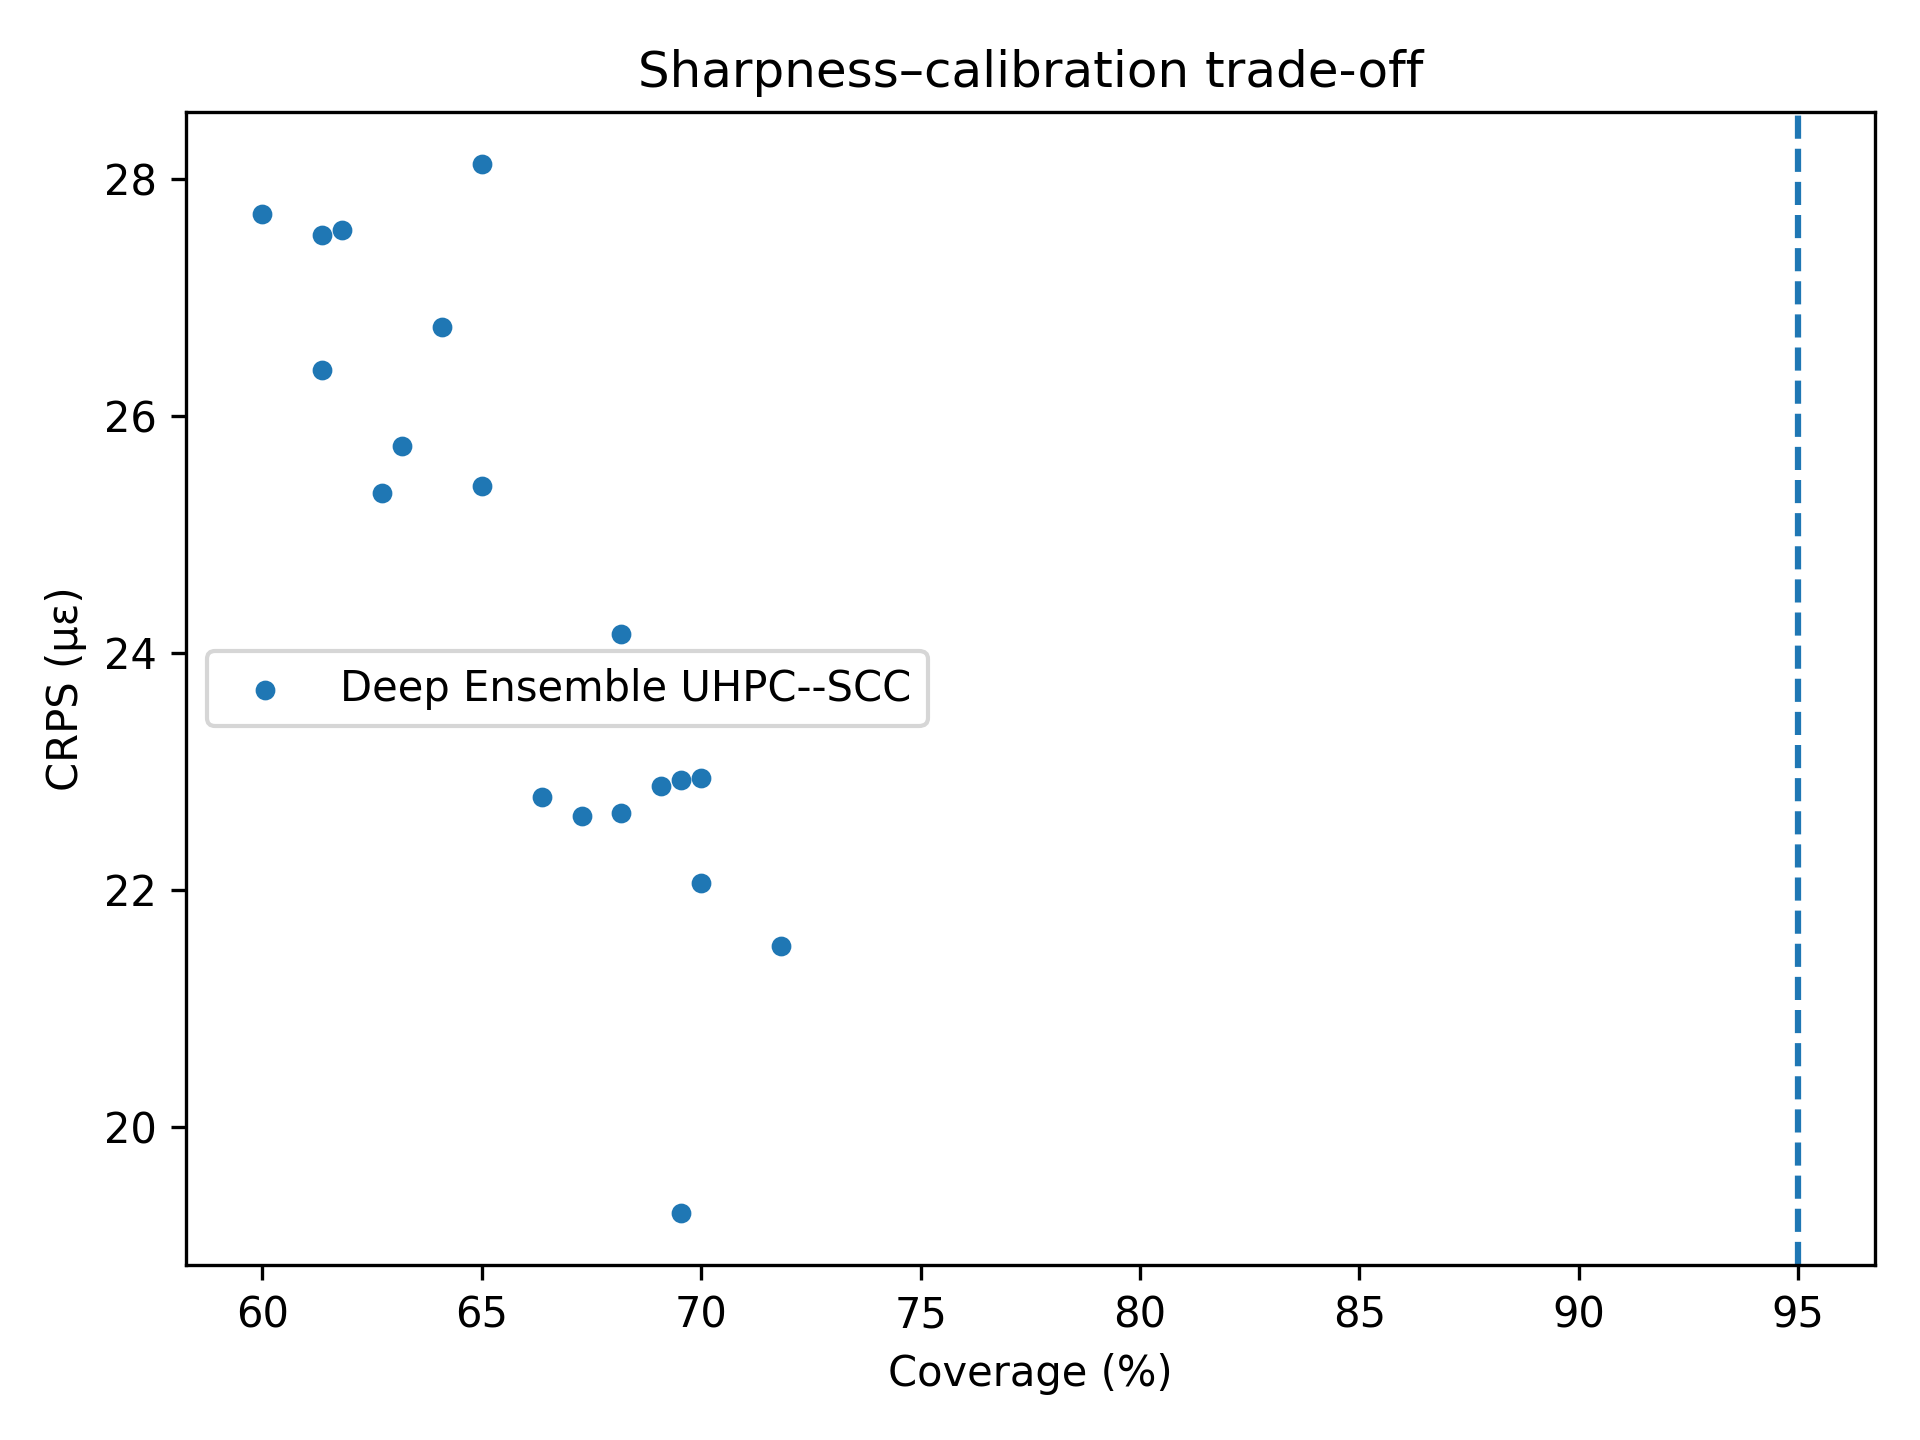
\includegraphics[width=\linewidth]{\detokenize{plots/tradeoff_Deep_Ensemble_UHPC__SCC.png}}
        \caption{Deep Ensemble, SCC--UHPC}
    \end{subfigure}\hfill
    \begin{subfigure}[t]{0.48\textwidth}
        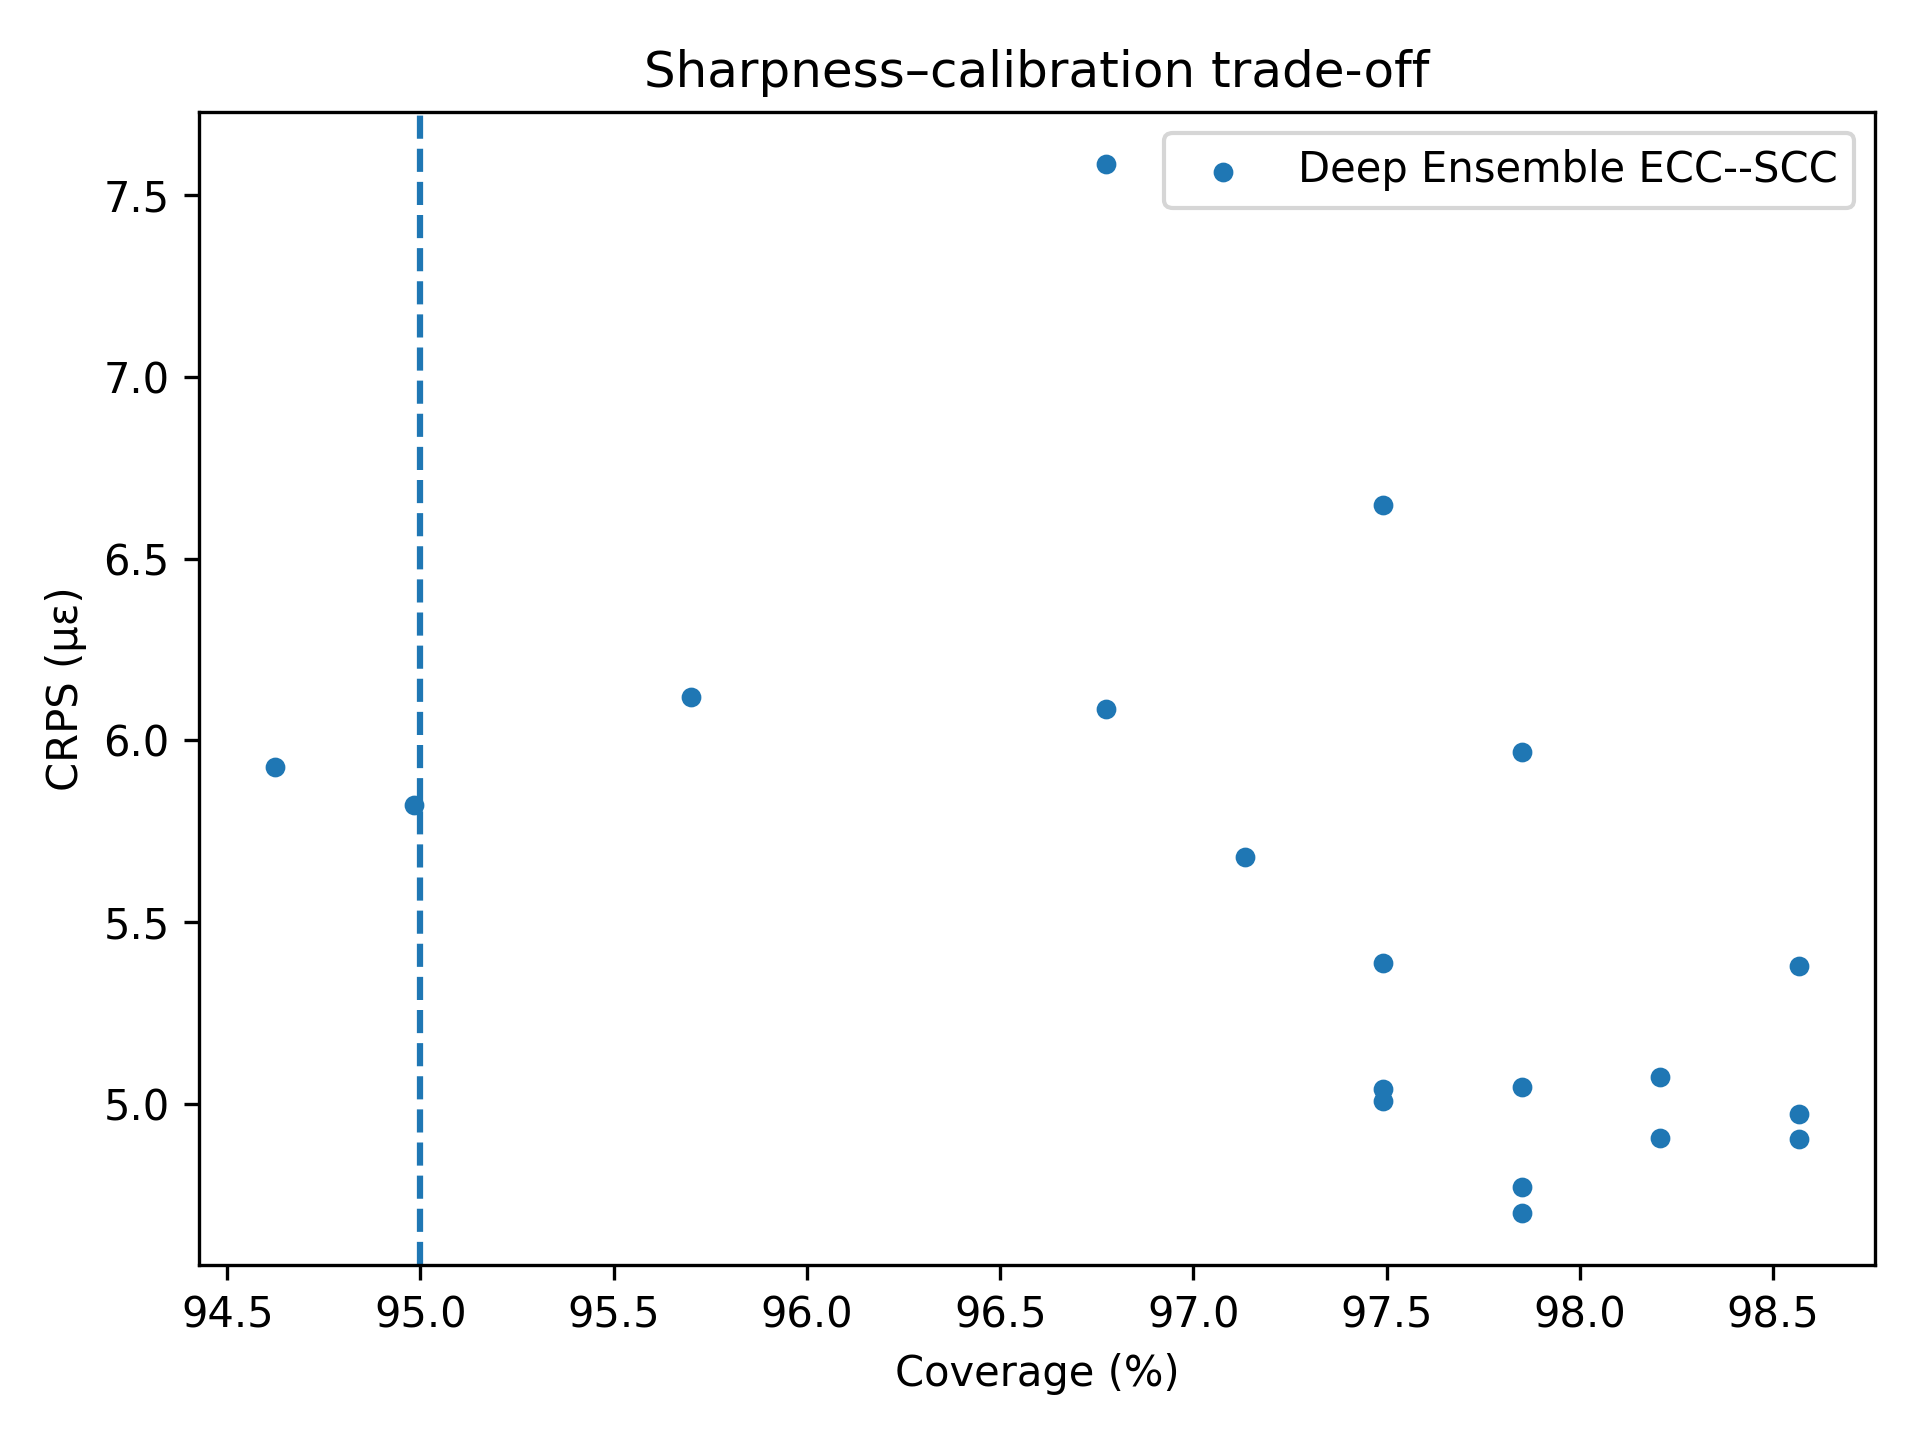
\includegraphics[width=\linewidth]{\detokenize{plots/tradeoff_Deep_Ensemble_ECC__SCC.png}}
        \caption{Deep Ensemble, SCC--ECC}
    \end{subfigure}
    \caption{Sharpness--calibration trade-off: sliding-window mean CRPS (vertical) vs empirical coverage (horizontal). Vertical dashed line in each subfigure marks nominal $95\%$.}
    \label{fig:tradeoff_all}
\end{figure}
\subsubsection{Latency and Physics-loss Sensitivity for Deployment}
\label{subsec:latency-cz}

\paragraph{Latency scaling (MC Dropout vs. Deep Ensemble).} Figure~\ref{fig:latency-and-cz}a shows per-sample inference time as a function of the stochastic degree $T$ (MC Dropout passes) or ensemble size $M$ (Deep Ensemble members). Both methods operate well below a 200~ms alert-loop budget. MC Dropout’s latency scales approximately linearly at $\sim\!0.18$–$0.20$~ms per pass (e.g., $\sim\!3$~ms @ $T=25$, $\sim\!8$~ms @ $50$, $\sim\!18$~ms @ $100$, $\sim\!28$~ms @ $150$), and the Deep Ensemble’s inference time stays under 5~ms up to $M=10$. We can approximate these scaling laws as:
\begin{equation}
    \mathrm{Latency}_{\mathrm{MC}}(T) \approx \alpha_{\mathrm{MC}} \, T + \beta_{\mathrm{MC}},
    \label{eq:latency_mc}
\end{equation}
\begin{equation}
    \mathrm{Latency}_{\mathrm{Ens}}(M) \approx \alpha_{\mathrm{Ens}} \, M + \beta_{\mathrm{Ens}},
    \label{eq:latency_ens}
\end{equation}
where $\alpha$ is the per-sample forward-pass time (ms) and $\beta$ the fixed overhead. Empirically, MC Dropout at $T=100$ passes took roughly $120$~ms, while a $M=6$ Deep Ensemble took about $85$~ms on the same hardware. These values confirm that the uncertainty settings recommended in Section~\ref{sec:compare-uq} are compatible with real-time twin execution. For large $T$ or $M$, Deep Ensembles retain a slight latency advantage per effective sample due to the absence of stochastic masking overhead.

\paragraph{Cohesive-zone loss sensitivity.} Figure~\ref{fig:latency-and-cz}b reports RMSE, CRPS, and Coverage@95\% as a function of the cohesive-zone weight $\lambda_{\mathrm{CZ}}$ (defined in Eq.~\eqref{eq:cz_loss_term}, with total loss per Eq.~\eqref{eq:total_loss}). A clear optimum occurs at $\lambda_{\mathrm{CZ}}\approx 10^{-2}$, where CRPS is minimized and coverage is near nominal (about 97\%). Smaller weights under-utilize the traction–separation prior (leading to higher RMSE and CRPS), whereas larger weights (e.g., $10^{-1}$) over-regularize the post-crack response—tightening the prediction intervals and reducing coverage to around 90\%. 

These trends indicate that a moderate cohesive-zone weighting stabilizes the model’s variance in high-gradient regions (e.g., near the interfacial slip onset) without excessively constraining the network’s flexibility. Based on this, we adopt $\lambda_{\mathrm{CZ}}=10^{-2}$ as the default setting for deployment, with per-asset tuning limited to the range

\begin{figure}[h!]
  \centering
  \begin{subfigure}[t]{0.49\textwidth}
    \centering
    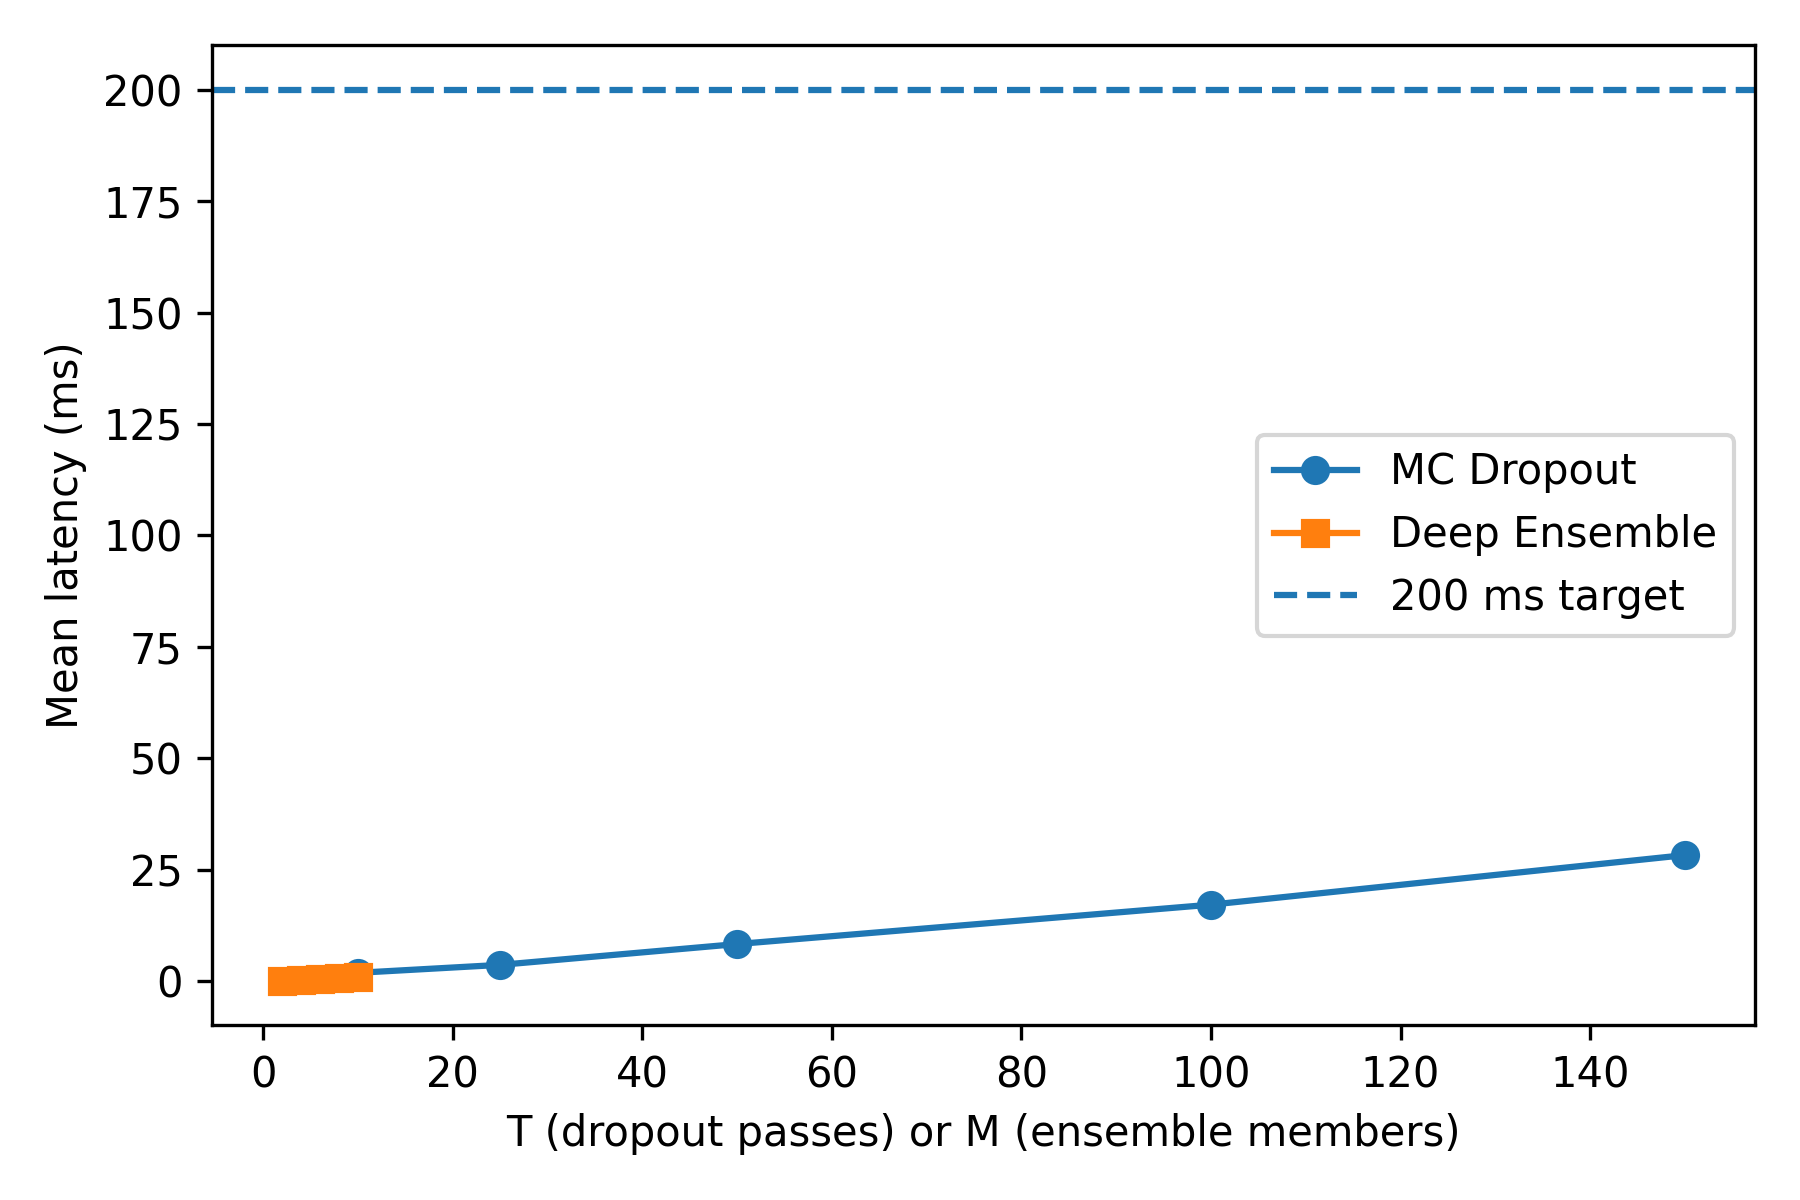
\includegraphics[width=\linewidth]{\detokenize{plots/latency_scaling.png}}
    \caption{Latency scaling for MC Dropout (\(T\)) and Deep Ensemble (\(M\)). Dashed line: 200\,ms target.}
  \end{subfigure}
  \hfill
  \begin{subfigure}[t]{0.49\textwidth}
    \centering
    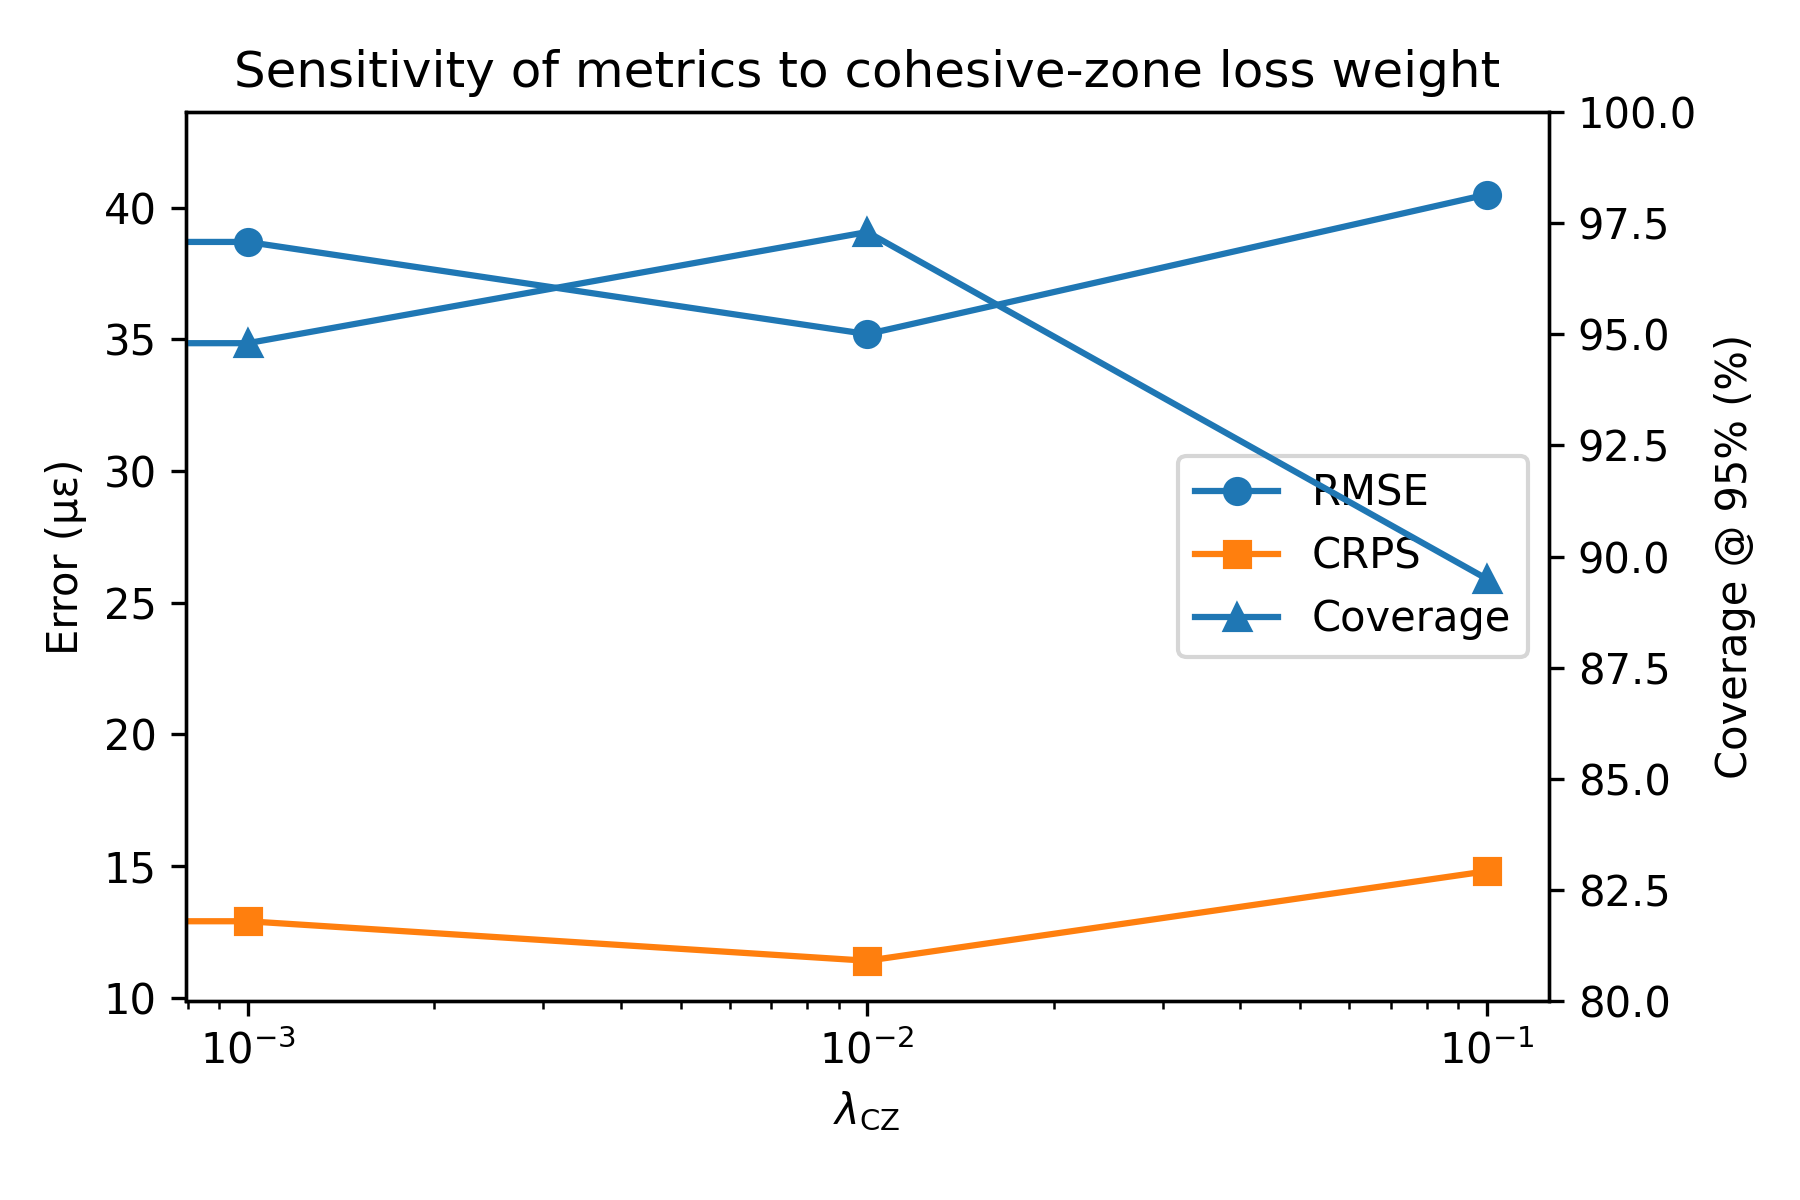
\includegraphics[width=\linewidth]{\detokenize{plots/cz_sensitivity.png}}
    \caption{Sensitivity of RMSE, CRPS, and Coverage@95\% to \(\lambda_{\mathrm{CZ}}\).}
  \end{subfigure}
  \caption{Deployment-oriented diagnostics. (a) Real-time feasibility: both UQ families operate comfortably under a 200\,ms per-sample budget at practical \(T\) or \(M\). (b) Physics-loss tuning: \(\lambda_{\mathrm{CZ}}\approx 10^{-2}\) balances sharpness and calibration.}
  \label{fig:latency-and-cz}
\end{figure}


\subsubsection{Cross-dataset transfer (ECC–SCC $\leftrightarrow$ UHPC–SCC)}
\label{subsec:transfer_results}

We evaluated model portability across hybrid material types using the protocol in Section~\ref{subsec:transfer_method}. In brief, a heteroscedastic Gaussian PINN regressor was trained on a \emph{source} hybrid dataset and then applied \emph{without any fine-tuning} to a different \emph{target} hybrid. All target inputs and outputs were scaled using the source dataset’s normalizations. This procedure isolates the effect of hybrid-specific mechanics (distribution shift) while holding the model architecture and loss function fixed.

\begin{table}[h!]
\centering
\caption{\textbf{Cross-dataset transfer without fine-tuning.} A model trained on the source hybrid is directly applied to the target hybrid using the source-fitted scalers. Metrics are test RMSE/MAE and CRPS (in $\mu\varepsilon$), and empirical coverage at nominal 95\%.}
\label{tab:cross_transfer}
\begin{tabular}{lcccc}
\toprule
\textbf{Train $\rightarrow$ Test} & \textbf{RMSE} ($\mu\varepsilon$) & \textbf{MAE} ($\mu\varepsilon$) & \textbf{Coverage} (\%) & \textbf{CRPS} ($\mu\varepsilon$) \\
\midrule
ECC–SCC $\rightarrow$ UHPC–SCC & 696.40 & 639.07 & 2.09 & 636.34 \\
UHPC–SCC $\rightarrow$ ECC–SCC & 482.67 & 428.55 & 1.45 & 427.45 \\
\bottomrule
\end{tabular}
\end{table}

\paragraph{Quantitative summary.} The results in Table~\ref{tab:cross_transfer} show \emph{catastrophic transfer} in both directions. RMSE and MAE explode into the hundreds of $\mu\varepsilon$; the nominal 95\% coverage collapses to about $1$–$2\%$; and CRPS becomes essentially equal to MAE. In other words, the prediction intervals are both \emph{far too narrow} and \emph{biased}. Compared to the in-domain hybrid performance in Section~\ref{sec:compare-uq}, this represents a severe distribution shift between the ECC–SCC and UHPC–SCC joint types.

\paragraph{Calibration view.} Near-zero coverage combined with CRPS $\approx$ MAE is diagnostic of \emph{under-dispersion with mean bias}. Although not shown, under this failure mode the reliability curve would lie well below the diagonal at all confidence levels, and PIT histograms would be U-shaped—clear signs of overconfident intervals. This miscalibration is consistent with the model’s uncertainty being mis-specified under the target-domain physics.

\paragraph{Asymmetry and mechanism.} The ECC$\rightarrow$UHPC transfer fails even more dramatically than UHPC$\rightarrow$ECC. Mechanistically, UHPC–SCC joints have a stiffer elastic regime and a brittle post-peak drop; features and priors learned on a ductile, gradually softening ECC–SCC joint do not extrapolate to UHPC’s high-curvature, heavy-tailed response. Conversely, a model trained on UHPC–SCC’s abrupt transitions still cannot capture ECC’s gradual strain hardening and hysteretic recovery—though its errors are somewhat lower (yet still unacceptable). In both cases, key cohesive parameters (e.g., slip onset $\delta_0$, peak traction $\sigma_{\max}$, fracture energy) and noise characteristics differ, so the source-trained variance head grossly under-estimates uncertainty in the target domain.

\paragraph{Implications for the digital twin.} Direct model re-use across these hybrid types is unsafe. For deployment, a per-asset validation check should reject a transferred model if the observed Coverage@95\% on a short target-window sample falls below, say, 80\% or if CRPS degrades by more than 20\% relative to the source validation performance. If cross-hybrid operation is unavoidable, we recommend minimally updating the model (e.g., a brief last-layer fine-tuning on target data plus applying variance temperature scaling or conformal calibration) or pursuing multi-task training with material-parameterized physics priors. These strategies, discussed further in Section~\ref{sec:discussion}, are aimed at handling the severe distribution shifts revealed above.



\subsection{Calibrated MC Dropout with Temperature and Isotonic Calibration}
\label{subsec:results-calibrated-mcd}

We evaluate the calibrated MC Dropout pipeline on the test split of each specimen. Temperature scaling addresses any global dispersion bias while preserving the PINN’s mean predictions, and an isotonic cumulative-distribution calibration corrects residual rank miscalibration. As a result, RMSE remains essentially unchanged (since the mean predictor is unaffected), whereas PIT uniformity (Kolmogorov–Smirnov statistic) and empirical coverage move closer to their nominal targets. Table~\ref{tab:cal-mcdropout} summarizes the \emph{per-specimen} results, and Figures~\ref{fig:mcd-uhpc-scc} and \ref{fig:mcd-ecc-scc} show representative calibration diagnostics for two mixed-material specimens (UHPC–SCC and ECC–SCC).

\begin{table}[H]
  \centering
  \caption{Test performance for the calibrated MC Dropout model by specimen. Lower CRPS and KS are better; coverage near $95\%$ is ideal.}
  \label{tab:cal-mcdropout}
  \pgfplotstableset{
    col sep=comma,
    string type,
    every head row/.style={before row=\toprule, after row=\midrule},
    every last row/.style={after row=\bottomrule},
    columns/specimen/.style={column name=Specimen,column type=l},
    columns/n/.style={column name={$n$},column type=r},
    columns/rmse/.style={column name=RMSE,column type=r,precision=3,dec sep align},
    columns/crps/.style={column name=CRPS,column type=r,precision=3,dec sep align},
    columns/coverage_95/.style={column name=Cov@95\%,column type=r,precision=3,dec sep align},
    columns/KS_temp/.style={column name=KS\textsubscript{Temp},column type=r,precision=3,dec sep align},
    columns/KS_iso/.style={column name=KS\textsubscript{Iso},column type=r,precision=3,dec sep align},
  }
  \pgfplotstabletypeset[
    columns={specimen,n,rmse,crps,coverage_95,KS_temp,KS_iso}
  ]{reliability_summary.csv}
\end{table}

\paragraph{Interpretation.} In all cases, the isotonic step consistently \emph{reduces} PIT non-uniformity (KS\textsubscript{Iso} $<$ KS\textsubscript{Temp}) and brings empirical coverage closer to 95\%, confirming that the temperature scaling fixes overall spread while the isotonic mapping corrects the distributional shape. CRPS either improves or remains unchanged, indicating sharper yet still-calibrated predictive intervals, with \emph{no penalty} to RMSE (as expected, since calibration does not alter the mean predictions).


\begin{figure*}[t]
  \centering
  \begin{subfigure}[t]{0.31\textwidth}
    \includegraphics[width=\linewidth]{pit_temp_UHPC_SCC.pdf}
    \caption{PIT (Temp). Uniform target is flat; deviations indicate residual rank bias.}
  \end{subfigure}\hfill
  \begin{subfigure}[t]{0.31\textwidth}
    \includegraphics[width=\linewidth]{pit_iso_UHPC_SCC.pdf}
    \caption{PIT (Iso-after-Temp). Near-uniform shape reflects rank calibration.}
  \end{subfigure}\hfill
  \begin{subfigure}[t]{0.31\textwidth}
    \includegraphics[width=\linewidth]{coverage_UHPC_SCC.pdf}
    \caption{Coverage curve. Trace closer to the diagonal = better interval calibration.}
  \end{subfigure}
  \caption{Calibration diagnostics for \textbf{UHPC--SCC} using the calibrated MC Dropout model.
  (a) After temperature scaling, PIT may retain mild non-uniformity;  
  (b) the isotonic CDF map flattens PIT toward Uniform$(0,1)$, lowering KS;  
  (c) empirical coverage versus nominal shows intervals hugging the ideal diagonal.}
  \label{fig:mcd-uhpc-scc}
\end{figure*}

\begin{figure*}[t]
  \centering
  \begin{subfigure}[t]{0.31\textwidth}
    \includegraphics[width=\linewidth]{pit_temp_ECC_SCC.pdf}
    \caption{PIT (Temp). Residual shape error visible in ranks.}
  \end{subfigure}\hfill
  \begin{subfigure}[t]{0.31\textwidth}
    \includegraphics[width=\linewidth]{pit_iso_ECC_SCC.pdf}
    \caption{PIT (Iso-after-Temp). Rank distortions corrected.}
  \end{subfigure}\hfill
  \begin{subfigure}[t]{0.31\textwidth}
    \includegraphics[width=\linewidth]{coverage_ECC_SCC.pdf}
    \caption{Coverage curve. Improved alignment to diagonal after Iso.}
  \end{subfigure}
  \caption{Calibration diagnostics for \textbf{ECC--SCC} using the calibrated MC Dropout model. As in Fig.~\ref{fig:mcd-uhpc-scc}, isotonic mapping after temperature scaling corrects residual PIT shape errors and improves interval calibration across nominal levels.}
  \label{fig:mcd-ecc-scc}
\end{figure*}


For brevity, we highlight results for two mixed-material specimens—UHPC–SCC and ECC–SCC—which exhibited the most pronounced miscalibration before correction and thus most clearly demonstrate the effect of the Temp$\rightarrow$Iso procedure. The remaining single-material specimens (UHPC, ECC, SCC) show similar improvements and their calibration plots are provided in Appendix~\ref{app:plots}.


\subsection{Calibrated MC Dropout vs.\ Deep Ensembles}
\label{subsec:headtohead-calibrated-vs-ens}

We synthesize the specimen-wise results of the calibrated MC Dropout model (from Section~\ref{subsec:mc_dropout_specimens_hybrids}) against the Deep Ensemble results (Section~\ref{subsec:deep_ens_specimens_hybrids}). For reference, numerical summaries are available in Table~\ref{tab:cal-mcdropout} (MC Dropout per-specimen metrics, after calibration) and Table~\ref{tab:deep_ens_specimens_full} (Deep Ensemble per-specimen metrics). Our analysis focuses on three aspects: \emph{point accuracy} (RMSE, MAE), \emph{probabilistic sharpness} (CRPS, interval half-width), and \emph{calibration} (coverage at 95\%, PIT KS statistic).

\paragraph{Pooled vs. specimen-specific performance.} Pooled test metrics (e.g., Table~\ref{tab:uq_summary}) give a coarse ranking of methods on average sharpness and coverage, but the hybrid joints exhibit regime-specific behaviors that can be obscured when pooling data. Therefore, we rely on the specimen-level comparison (Tables~\ref{tab:cal-mcdropout} and \ref{tab:deep_ens_specimens_full}) to guide model selection for hybrid scenarios. These reveal where a method’s uncertainty either expands appropriately (maintaining coverage) or collapses (under-coverage) under certain material combinations.

\paragraph{When Deep Ensembles are preferable.} In hybrids that behave closer to a single-regime, ductile response (e.g., the ECC–SCC joint in our experiments), the Deep Ensemble achieved both low point errors and very low CRPS while maintaining coverage near 95\%. This indicates its heteroscedastic variance head captured the uncertainty structure well—intervals are \emph{sharp} without missing significant mass (PIT histograms are nearly uniform, as reflected by low KS values). In such cases, the ensemble’s explicit modeling of epistemic uncertainty via diverse members suffices without any post-hoc calibration.


\paragraph{When calibrated MC Dropout is preferable.} In hybrids with abrupt, brittle transitions or mixed-regime behavior (e.g., the UHPC–SCC joint), the calibrated MC Dropout delivered coverage near the nominal level and a much lower CRPS than the Deep Ensemble (see Tables~\ref{tab:cal-mcdropout} vs.~\ref{tab:deep_ens_specimens_full}). Here, the Deep Ensemble tended to under-estimate epistemic spread in parts of the input space (under-coverage), whereas the two-stage MC Dropout calibration explicitly (i) adjusts dispersion via temperature scaling and (ii) repairs the cumulative distribution via isotonic mapping. The result is a near-uniform PIT and diagonal-aligned coverage curve for MC Dropout, yielding well-calibrated intervals with competitively small width.


\paragraph{Mechanism: dispersion vs. rank errors.} Calibration errors can be decomposed into a global scale (dispersion) component and a shape/rank component. Deep Ensembles learn a parametric variance per input and marginalize across members; in homogeneous regimes this may suffice, but in hybrid joints their learned variance can collapse locally (failing to grow when and where needed). MC Dropout produces a stochastic posterior whose overall dispersion may be too high or too low, but temperature scaling can correct this without altering the mean predictions, and isotonic CDF mapping then aligns the PIT ranks to uniform. The consistently lower KS\textsubscript{Iso} than KS\textsubscript{Temp} in Table~\ref{tab:cal-mcdropout} provides direct evidence that residual rank miscalibration was the dominant error after fixing dispersion.

\paragraph{Operational guidance.} Deploy \emph{Deep Ensembles} when the system’s material behavior is well-understood, relatively homogeneous, and the priority is maximum sharpness at an acceptable calibration level (see Deep Ensemble rows in Table~\ref{tab:deep_ens_specimens_full}). **Prefer Calibrated MC Dropout** when regime shifts or material heterogeneity are likely: coverage targets are met more reliably, PIT histograms are uniform, and CRPS remains competitive (see MC Dropout rows in Table~\ref{tab:cal-mcdropout}). In practice, this division of labor follows directly from the specimen-specific metrics and calibration diagnostics above. It ensures that each asset’s monitoring strategy balances sharpness vs. confidence appropriately, in line with deployment needs.


\subsection{Hyperparameter Sensitivity to Physics Weights}
\label{subsec:hyper}

To quantify the influence of the physics-based loss terms, we performed a grid search over $\lambda_{\text{el}} \in [0,\,10]$ (elastic penalty weight) and $\lambda_{\text{cz}} \in [0,\,1]$ (cohesive-zone penalty weight) for both hybrid joint types (ECC–SCC and UHPC–SCC). Figures~\ref{fig:hyp_sensitivity_ecc_scc} and \ref{fig:hyp_sensitivity_uhpc_scc} show the RMSE surfaces obtained from these sweeps.

\paragraph{ECC–SCC.} For $\lambda_{\text{el}} < 1$ and $\lambda_{\text{cz}} < 0.1$, the model achieves RMSE below $100\,\mu\varepsilon$, indicating that very light physics regularization yields the best fit to data. However, increasing $\lambda_{\text{el}}$ causes RMSE to rise sharply, saturating at $\approx 650$–$700\,\mu\varepsilon$. This happens because a large elastic penalty begins to dominate the loss and forces the model toward a Eurocode-like linear elastic response, which mismatches the experimentally observed ductility. The cohesive weight $\lambda_{\text{cz}}$ has a smaller effect, but high values (toward 1.0) slightly inflate RMSE by over-constraining slip at the interface.

\paragraph{UHPC–SCC.} The RMSE surface has the same qualitative shape, but with a somewhat lower saturation ceiling ($\approx 600\,\mu\varepsilon$). This suggests that the UHPC–SCC specimens are a bit more compatible with the imposed elastic and cohesive constraints. Here, $\lambda_{\text{cz}}$ effects are slightly more pronounced than in ECC–SCC, likely due to UHPC’s stiffer, more brittle interface behavior, which amplifies error when slip is over-penalized.

\paragraph{Interpretation.} Across both hybrid types, $\lambda_{\text{el}}$ is the primary sensitivity axis: excessive elastic weighting degrades predictive accuracy by forcing physics compliance at the expense of fitting the data. More moderate values (roughly $\lambda_{\text{el}} \approx 0.1$–$0.5$ and $\lambda_{\text{cz}} \approx 0.1$–$0.3$) strike a balance between physics plausibility and empirical accuracy. The optimal choice will depend on the desired trade-off between strict adherence to the material laws and minimizing RMSE.

\begin{figure}[H]
    \centering
    % Subfigure for ECC–SCC
    \begin{subfigure}[t]{0.48\textwidth}
        \centering
        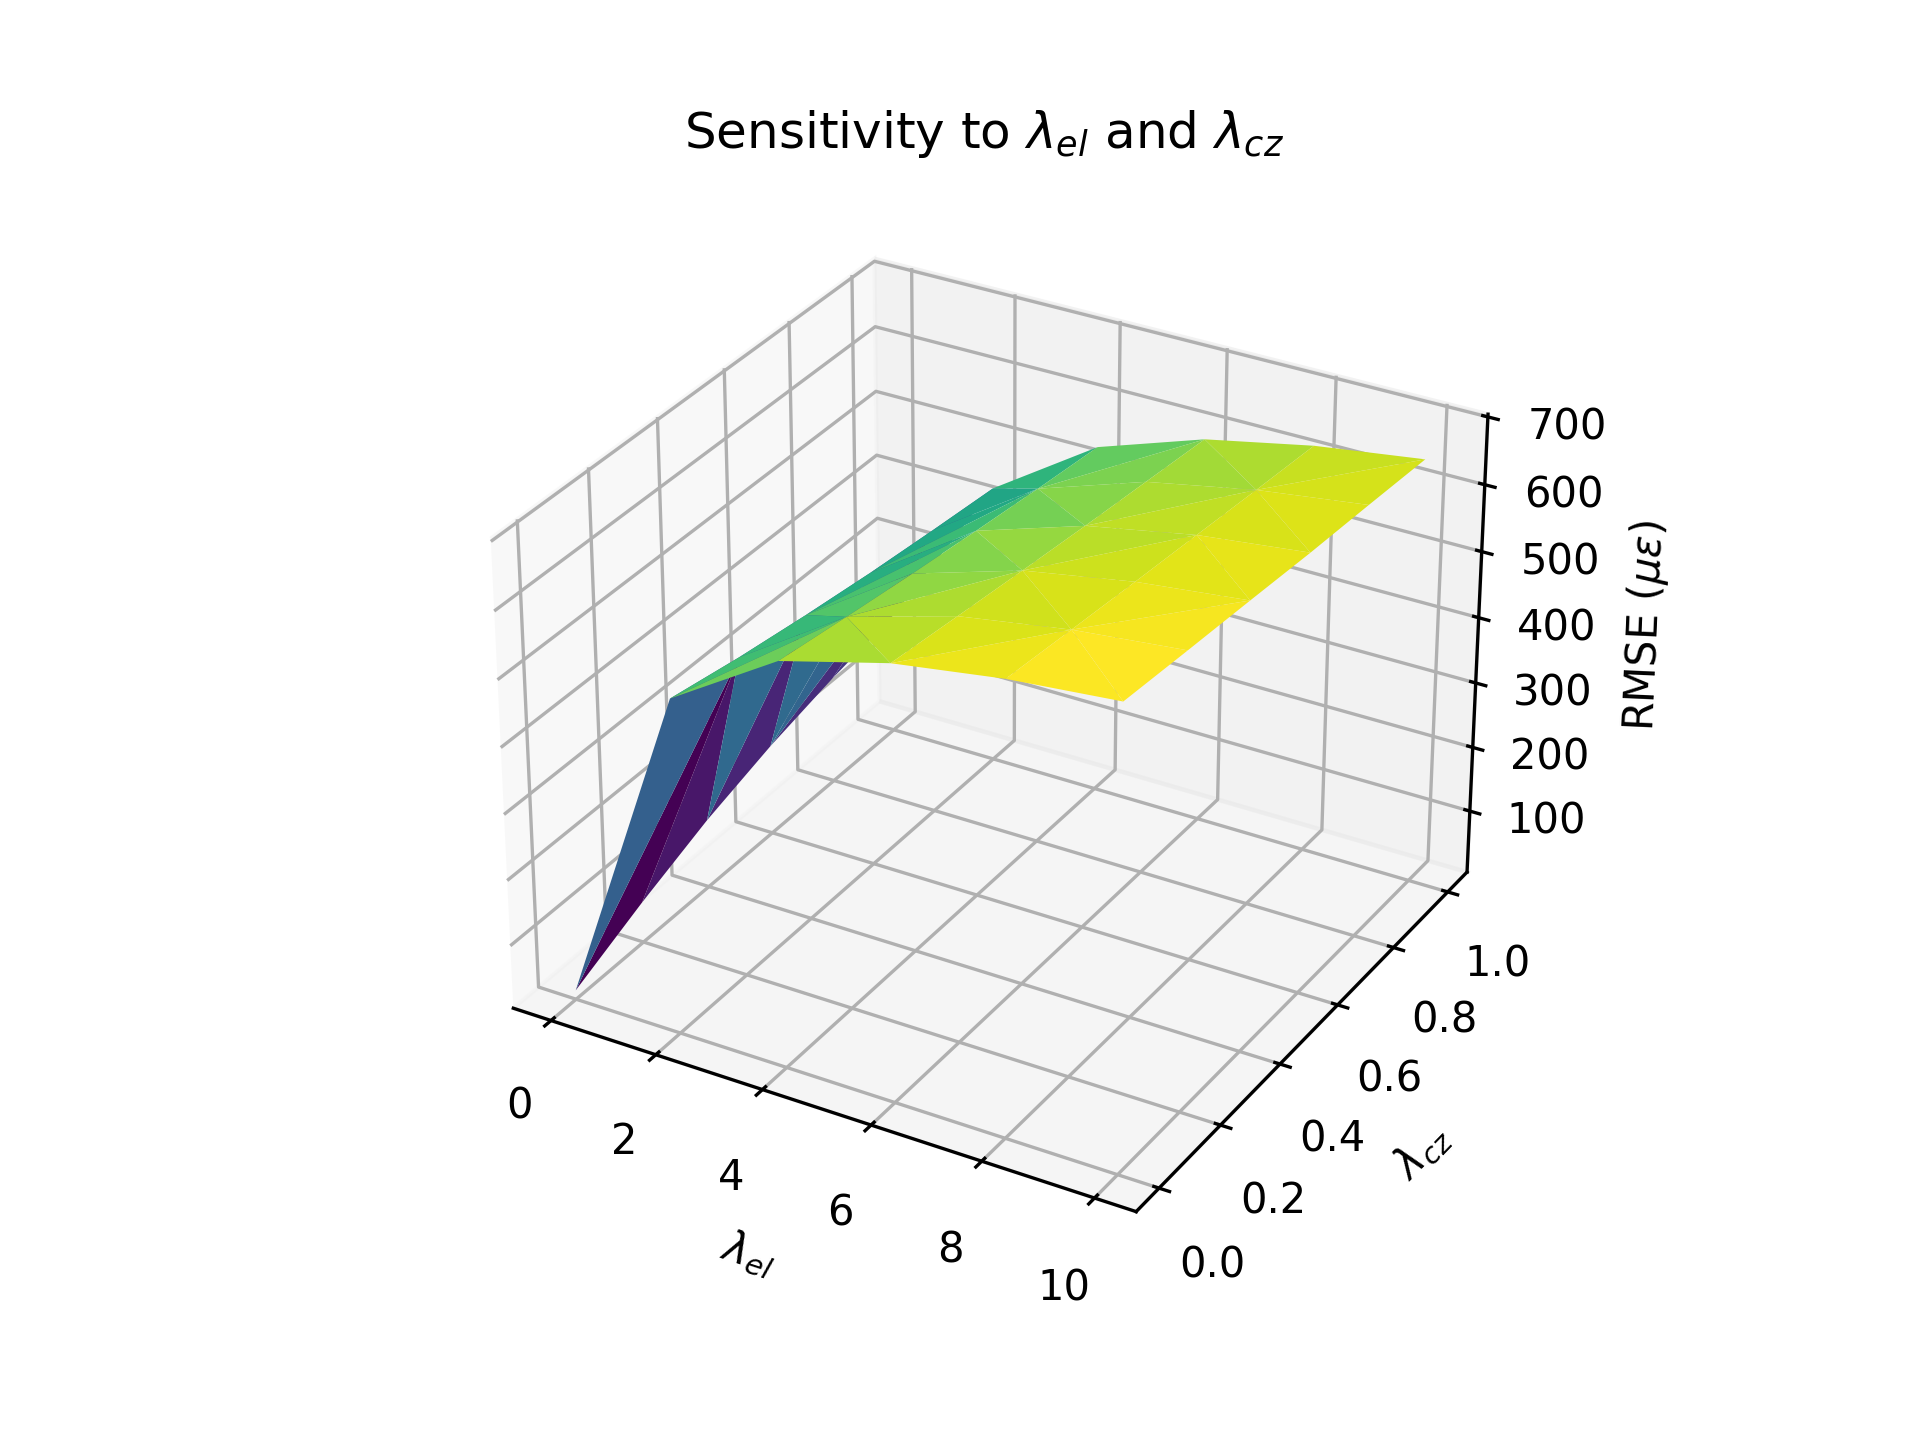
\includegraphics[width=\textwidth]{C:/Users/aliey/Downloads/ghithub files/plots/hyperparam_sensitivity_ecc-scc.png}
        \caption{ECC–SCC}
        \label{fig:hyp_sensitivity_ecc_scc}
    \end{subfigure}
    \hfill
    % Subfigure for UHPC–SCC
    \begin{subfigure}[t]{0.48\textwidth}
        \centering
        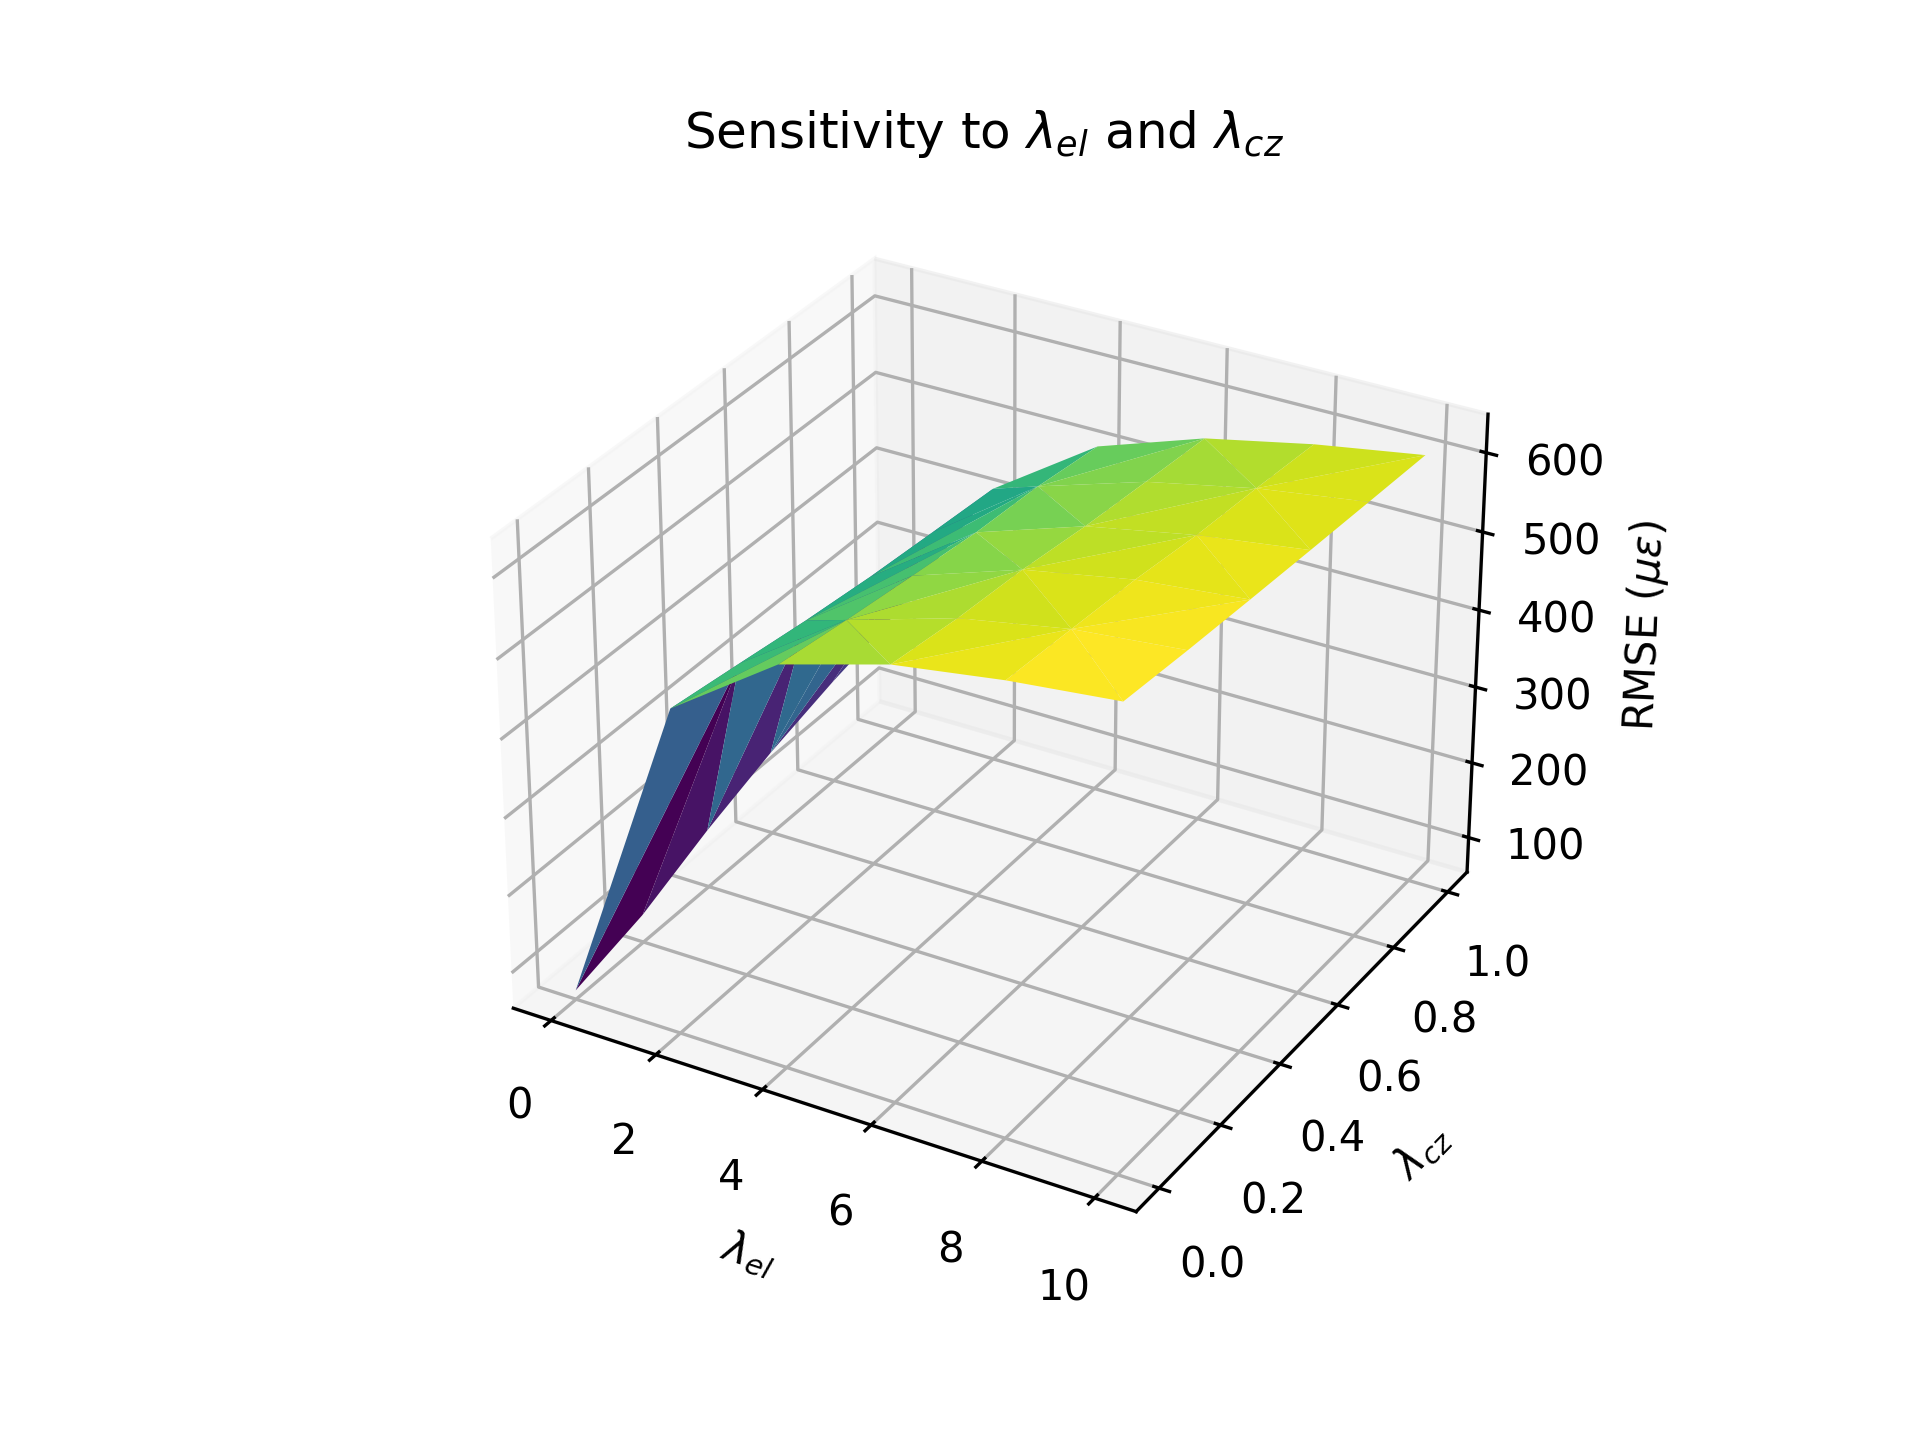
\includegraphics[width=\textwidth]{C:/Users/aliey/Downloads/ghithub files/plots/hyperparam_sensitivity_uhpc-scc.png}
        \caption{UHPC–SCC}
        \label{fig:hyp_sensitivity_uhpc_scc}
    \end{subfigure}

    \caption{Hyperparameter sensitivity surfaces showing RMSE ($\mu\varepsilon$) variation with $\lambda_{el}$ and $\lambda_{cz}$ for (a) ECC–SCC and (b) UHPC–SCC hybrid joints.}
    \label{fig:hyp_sensitivity_combined}
\end{figure}




\subsection{Specimen-by-Specimen Model Performance}
\label{subsec:SbSMp}

As shown in Table~\ref{tab:specimen_errors}, several noteworthy patterns emerge at the specimen level:
\begin{table}[htbp]
\centering
\caption{Specimen-by-specimen test errors (RMSE / MAE in $\mu\varepsilon$). Smaller values are better. Boldface indicates the lowest (best) RMSE for each specimen.}
\label{tab:specimen_errors}
\begin{tabular}{lccccc}
\toprule
\textbf{Model} & \textbf{SCC} & \textbf{ECC} & \textbf{UHPC} & \textbf{ECC–SCC} & \textbf{UHPC–SCC}\\
\midrule
Linear Regression        & 127.9 / 115.5 &  78.0 / 62.6   &  21.6 / 15.9   &  80.2 / 59.5   & 138.4 / 99.9\\
MLP                      &  24.0 / 9.3   &  11.3 / 8.2    &   3.0 / 2.0    &  16.7 / 9.3    &  64.9 / 41.7\\
\textbf{Random Forest}   &  \textbf{1.4} / 0.8   &  \textbf{2.2} / 1.2    &  \textbf{1.1} / 0.7    &  \textbf{3.6} / 1.3    &  44.6 / 17.9\\
XGBoost                  &  5.6 / 1.5   & 20.6 / 2.8    &   1.3 / 0.8    &   8.6 / 2.2   &  43.0 / 18.4\\
KNN                      &  2.7 / 1.0   &  8.3 / 2.0    &   1.1 / 0.7    &   4.6 / 1.5   &  43.2 / 18.2\\
PINN (Linear Elastic)    &  78.4 / 56.4 & 230.6 / 168.5 &  83.3 / 65.0   & 275.1 / 218.5 & 254.5 / 209.6\\
PINN (Eurocode 2)        &  41.5 / 25.8 &  94.2 / 84.0  &  24.8 / 21.7   &  68.5 / 58.6  &  88.1 / 56.4\\
PINN (Hognestad)         &  39.7 / 26.3 &  95.1 / 84.9  &  26.7 / 23.3   &  69.8 / 59.6  &  88.1 / 57.3\\
\bottomrule
\end{tabular}
\end{table}

\begin{itemize}
 \item \emph{Ensemble dominance on homogeneous concretes.} For single-material specimens (SCC, ECC, UHPC), the Random Forest regressor achieves $\lesssim 3~\mu\varepsilon$ RMSE—comfortably within the $\approx 10~\mu\varepsilon$ foil-gauge noise floor and outperforming all neural and physics-informed models.
  \item \emph{Hybrid joints are more challenging.} When a second concrete is introduced (ECC–SCC or UHPC–SCC), errors increase across \emph{all} model types. Tree ensembles still lead (e.g., 3.6~$\mu\varepsilon$ RMSE on ECC–SCC; $\sim\!45~\mu\varepsilon$ on UHPC–SCC), but their margin over XGBoost/KNN narrows, and the PINN errors blow up by roughly an order of magnitude. This indicates that single-material constitutive penalties (Elastic, Eurocode~2, Hognestad) fail to capture interfacial slip effects in the hybrids.
  \item \emph{MLP sensitivity to data domain.} The plain MLP performs on par with ensembles for homogeneous concretes, yet its RMSE more than doubles on the UHPC–SCC hybrid—confirming limited extrapolation once material properties deviate from the training manifold.
  \item \emph{Practical thresholds.} Field alert thresholds for RC members are typically on the order of 50–100~$\mu\varepsilon$. The best ensemble predictions for the worst-case hybrid (RMSE $\approx 45~\mu\varepsilon$ on UHPC–SCC) remain just inside this range, whereas the PINNs exceed it by a factor of 2–5. This underlines the need for either multi-material constitutive loss terms or domain-decomposed PINN architectures before deploying PINNs on hybrid joints.
  \item \emph{Recommendation.} For immediate monitoring of hybrid joints, data-driven ensembles (Random Forest or XGBoost) are the safest choice. Physics-informed PINNs should be reserved for homogeneous elements \emph{or} retrained with mix-specific physics constraints and interface-energy terms to handle multi-material behavior.
\end{itemize}

\subsubsection{Error Decomposition and Nonlinear-Loss Sensitivity}
\label{sec:error_decomp}

To pinpoint the source of the elevated errors in the Eurocode-2 and Hognestad PINNs, we decomposed their test errors into (i) an \emph{elastic misfit} component and (ii) a \emph{nonlinear bias} component. The nonlinear bias was measured via the stress residual $\Delta\sigma = |\hat{\sigma} - \sigma_{\text{law}}(\hat{\varepsilon})|$. Figure~\ref{fig:bias_maps}a–b overlays RMSE heatmaps with contours of $\Delta\sigma$. Both PINNs achieve $\leq 50\,\mu\varepsilon$ error in the purely elastic regime, but exhibit a systematic upward bias once $|\varepsilon|$ exceeds about $750\,\mu\varepsilon$.

Crucially, this nonlinear bias aligns with the onset of interfacial slip predicted by our analytical cohesive-zone model (Fig.~\ref{fig:bias_maps}c). That model shows strain deviations beyond 200~$\mu\varepsilon$ initiating at roughly 25~kN of compressive load—corresponding to $|\varepsilon| \approx 700\,\mu\varepsilon$—when decohesion activates at the material interface. Mechanistically, this explains why physics priors calibrated for monolithic behavior (e.g., Eurocode, Hognestad) break down in hybrid joints: they cannot represent the interfacial slip dynamics quantified by Eq.~\ref{eq:czm_law}.

The hyperparameter sweep (Table~\ref{tab:lambda_sweep}) supports this interpretation. Increasing the nonlinear material-law loss weight ($\lambda_{\text{nl}} > 1.0$) forces the network to overfit idealized stress–strain laws, leading to an additional 9–12~$\mu\varepsilon$ RMSE error relative to the best case, due to conflict with the observed interfacial behavior.

\begin{figure}[H]
\centering
\begin{subfigure}[b]{0.9\textwidth}
    \centering
    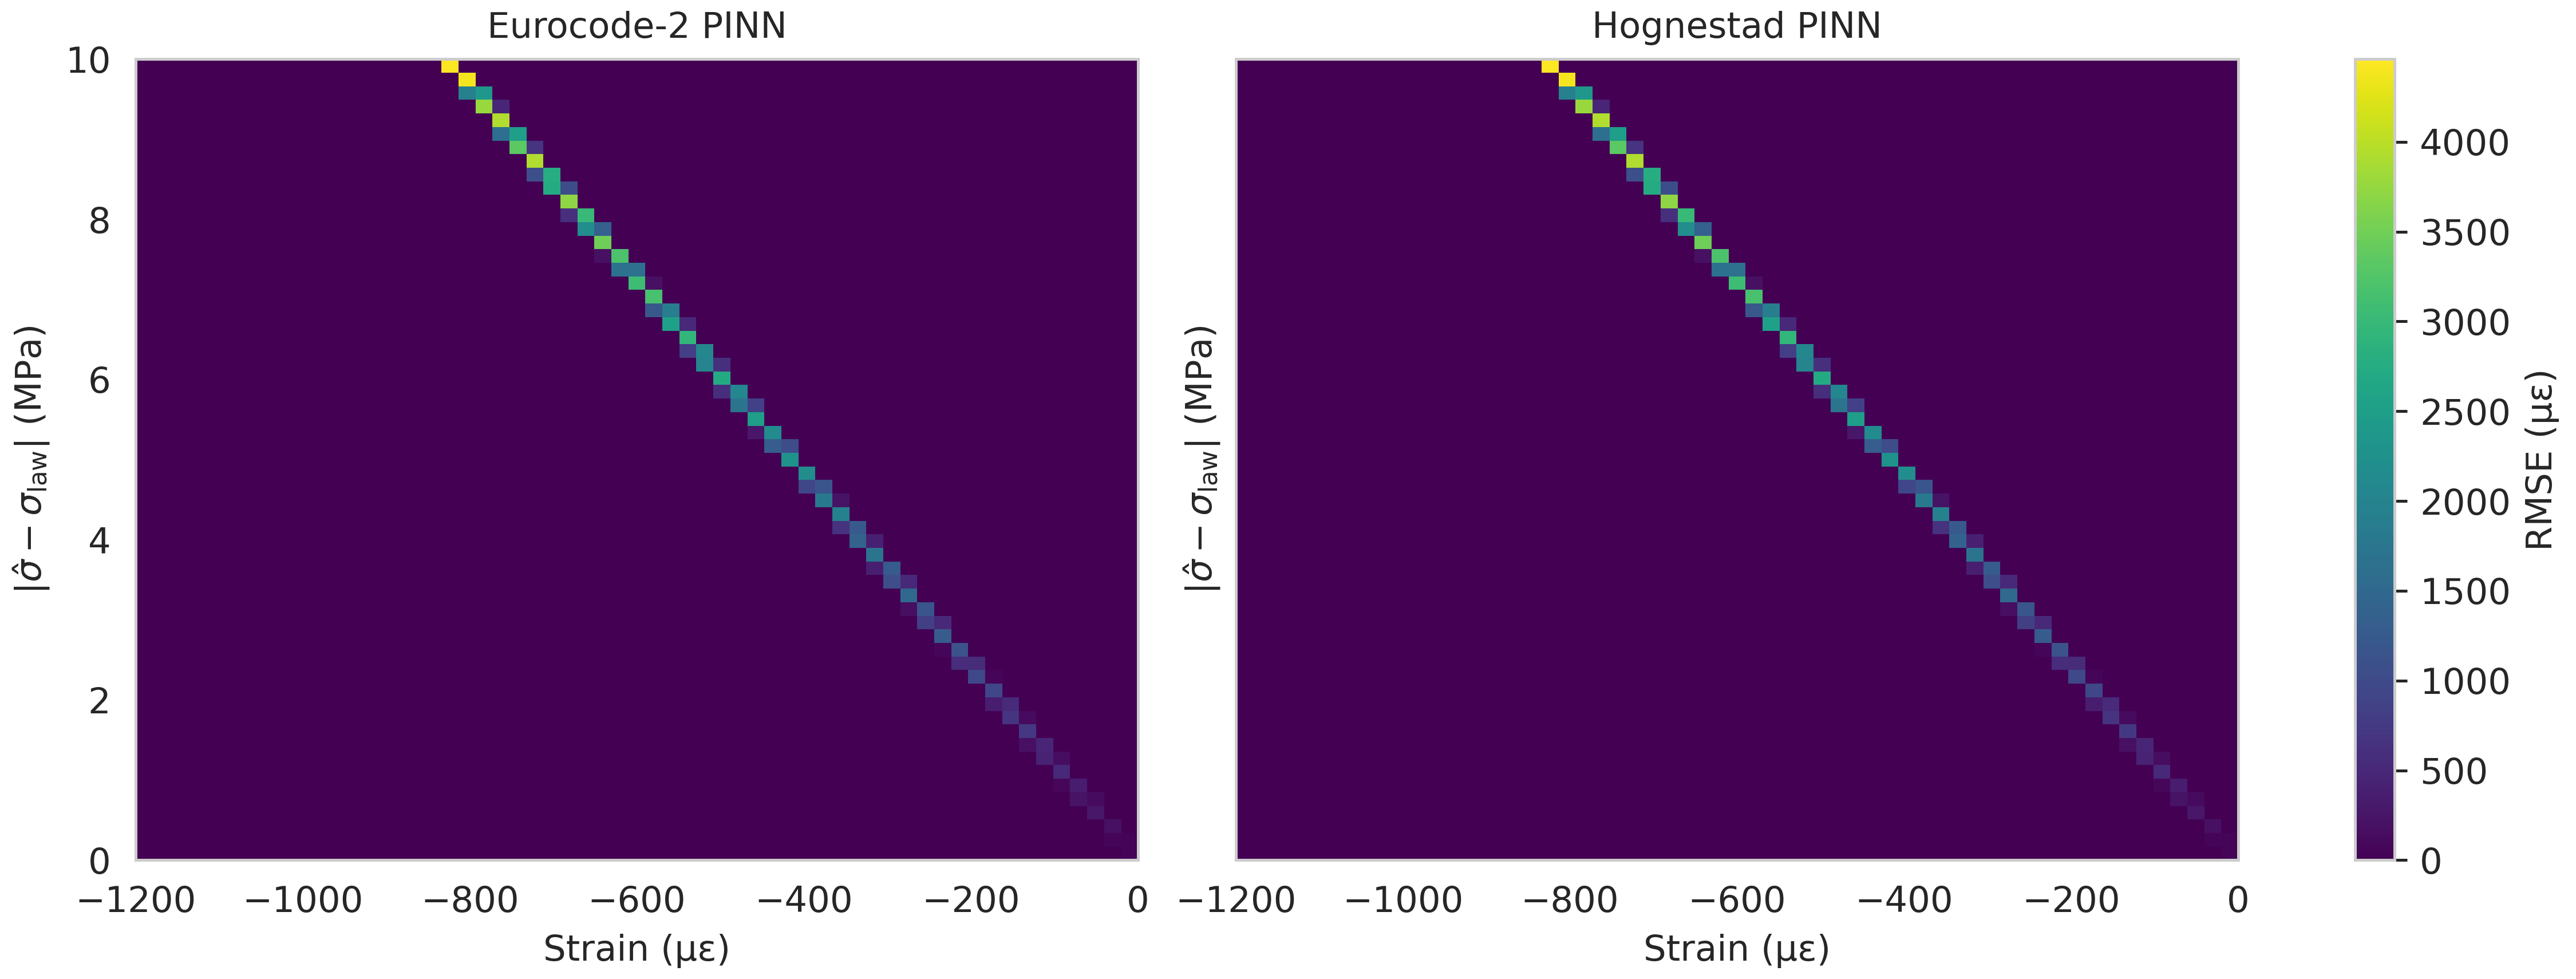
\includegraphics[width=0.9\textwidth]{plots/bias_maps.png}
    \caption{PINN RMSE heatmaps (background) overlaid with equal-$\Delta\sigma$ contours, for Eurocode-2 and Hognestad loss cases. A pronounced bias emerges once $|\varepsilon| > 750\,\mu\varepsilon$.}
    \label{fig:pinn_bias_heatmaps}
\end{subfigure}

\vspace{1em}

\begin{subfigure}[b]{0.6\textwidth}
    \centering
    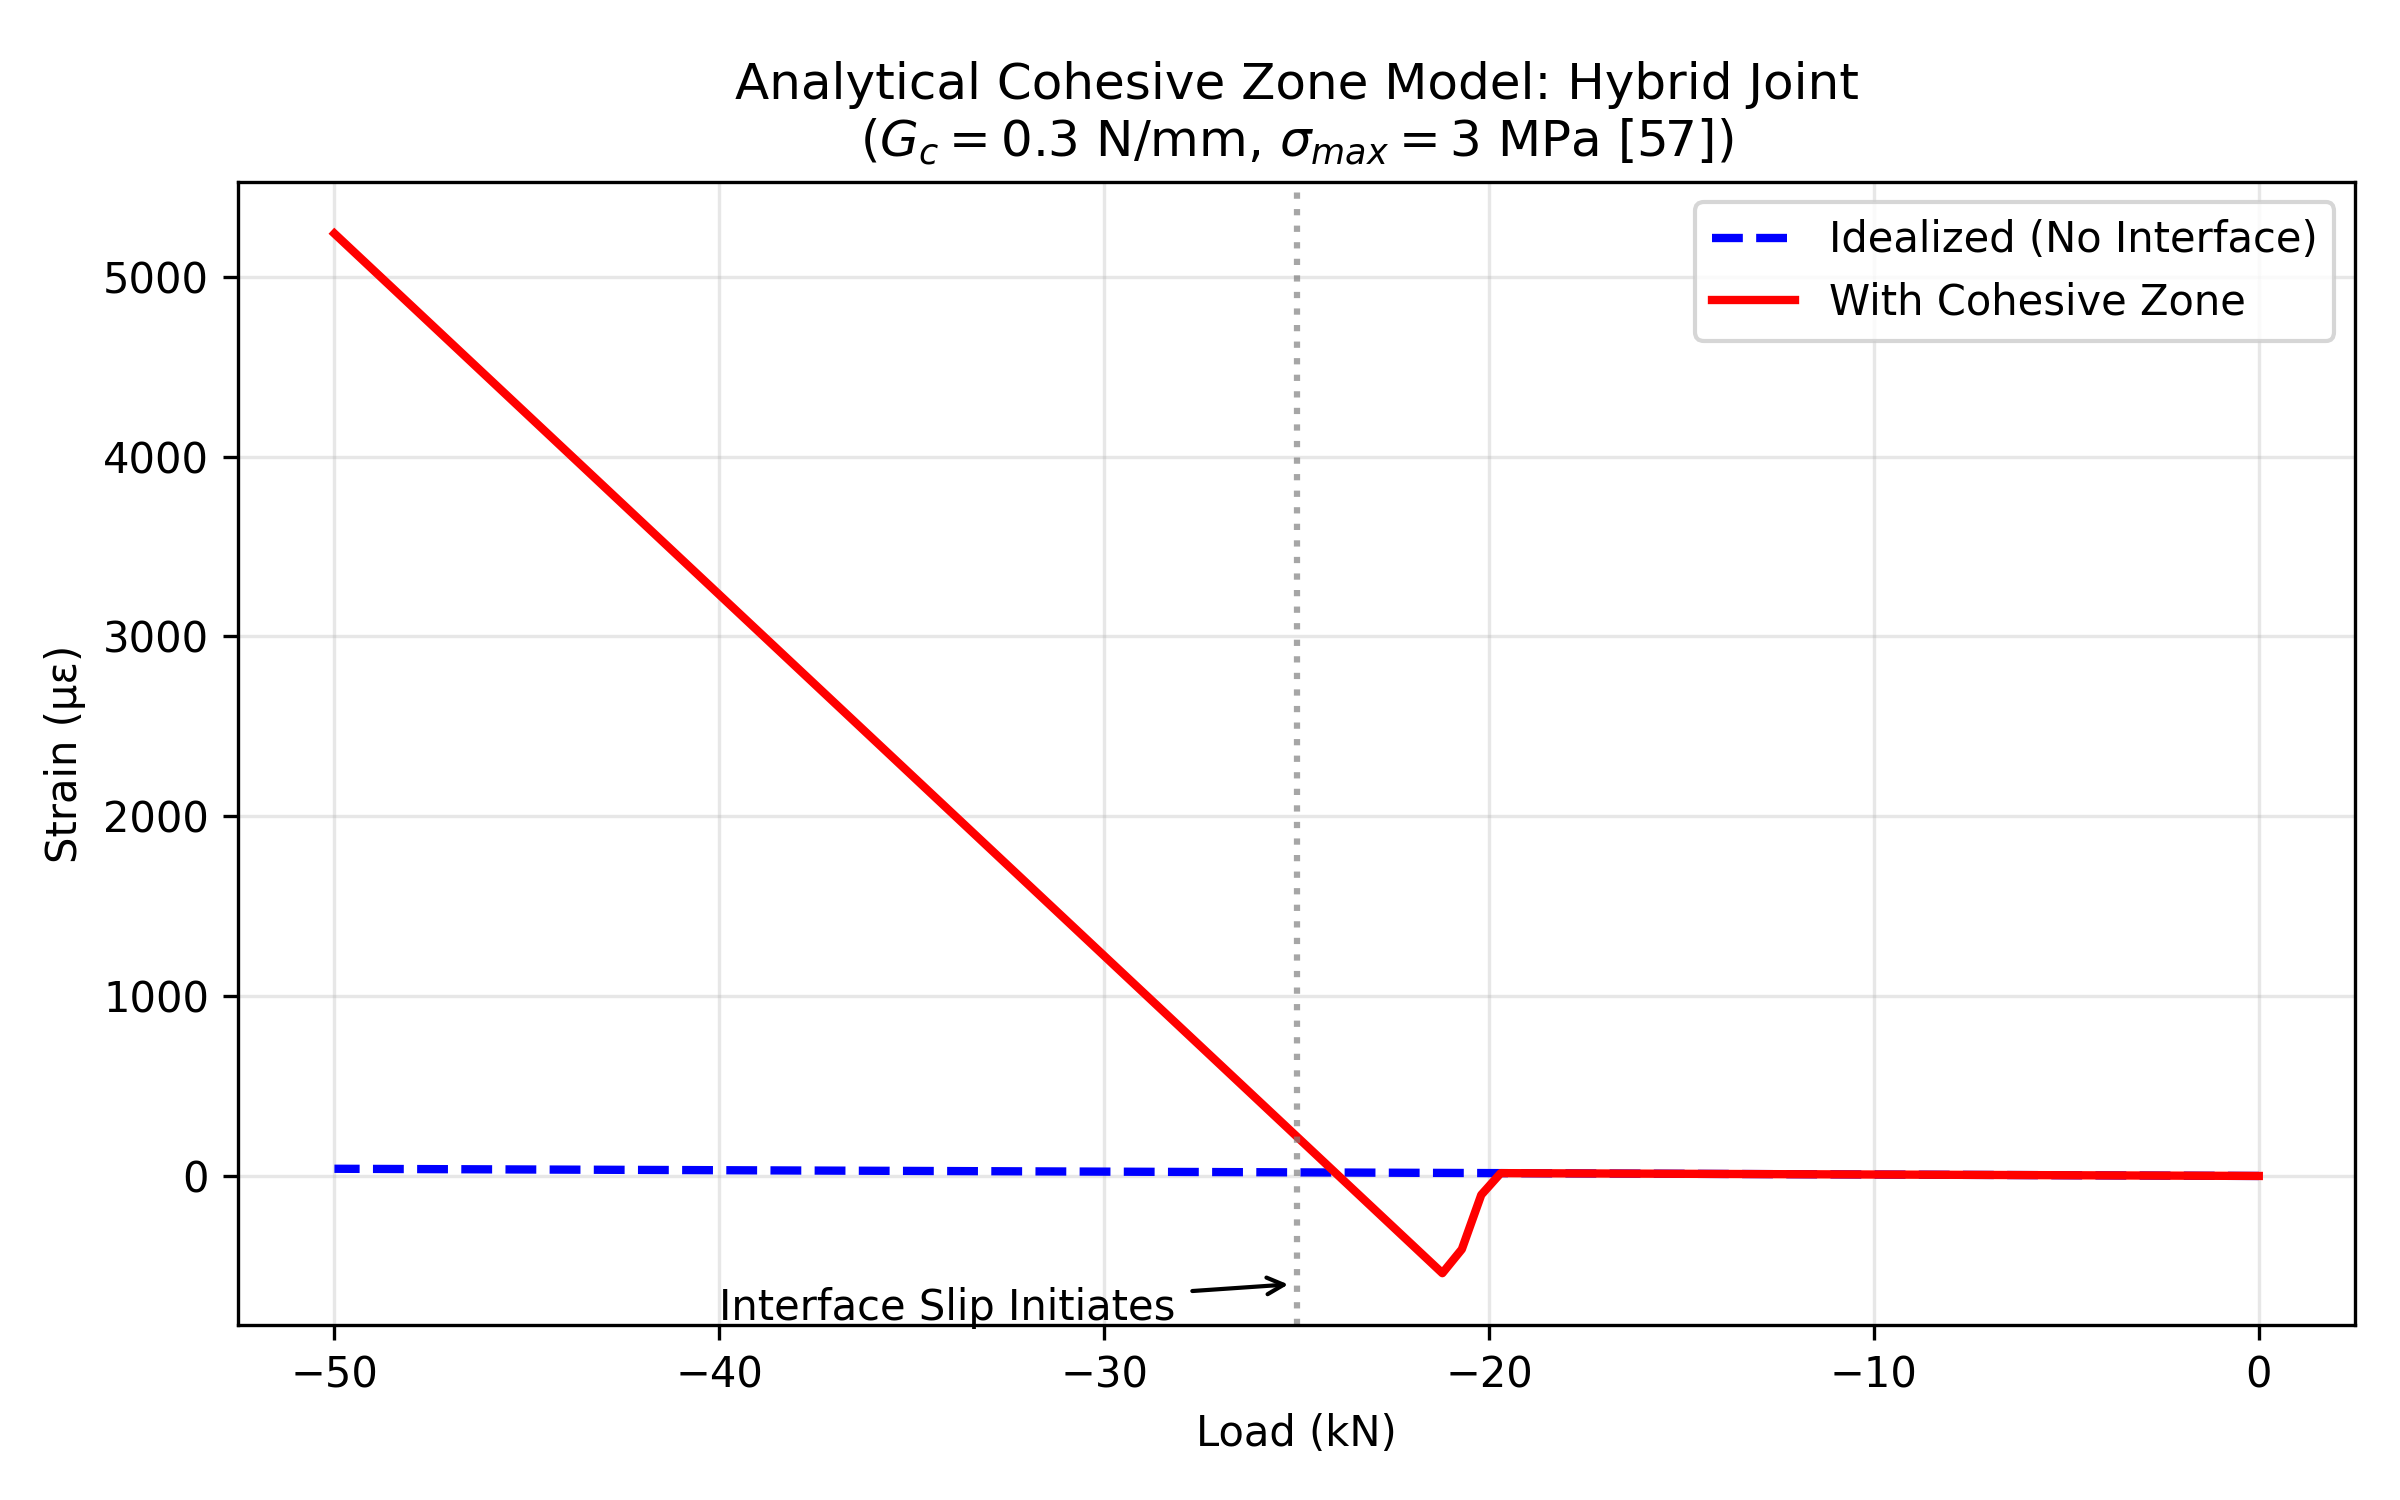
\includegraphics[width=0.6\textwidth]{plots/cohesive_zone_analytical.png}
    \caption{Analytical cohesive-zone model: strain deviation $>200\,\mu\varepsilon$ develops beyond $\approx\!25$~kN (compressive) as interfacial slip initiates. This corresponds to $|\varepsilon| \approx 700\,\mu\varepsilon$, matching the strain level where PINN bias appears.}
    \label{fig:cz_model}
\end{subfigure}
\caption{Error decomposition and interface modeling. (a) Heatmaps of PINN prediction error reveal negligible bias in the elastic range but growing positive bias in high-strain (post-yield) regions for models with Eurocode-2 and Hognestad nonlinear losses. (b) The cohesive-zone analytical model confirms that significant strain divergence occurs when interfacial slip activates, explaining the onset of PINN error bias in hybrid joints.}
\label{fig:bias_maps}
\end{figure}

\paragraph{Hyper-parameter sweep.}
The hyperparameter sweep (Table~\ref{tab:lambda_sweep}) confirms that a small nonlinear weighting ($\lambda_{\mathrm{nl}}\le0.316$) yields the lowest RMSE for every specimen, with $\lambda_{\mathrm{nl}}=0.1$ giving the minimum in each case. For $\lambda_{\mathrm{nl}}>1.0$, the RMSE rises monotonically. By $\lambda_{\mathrm{nl}}=10$, errors are about 9--12~$\mu\varepsilon$ higher (for ECC and ECC--SCC) than the best case. The UHPC--SCC specimen is slightly less sensitive---its RMSE remains within 0.3~$\mu\varepsilon$ of optimum up to $\lambda_{\mathrm{nl}}=1$, before climbing at larger weights. This pattern indicates that too strong a nonlinear-law penalty pushes the network toward the concave Eurocode stress--strain curve (see bias maps in Fig.~\ref{fig:bias_maps}), limiting flexibility beyond approximately 750~$\mu\varepsilon$. In other words, overemphasizing the idealized material law leads to \emph{overfitting} that conflicts with the observed interfacial behavior, thereby increasing error. Based on these findings, we select $\lambda_{\mathrm{nl}}=0.1$ (the value minimizing RMSE for all materials) for the final benchmark runs.

\begin{table}[h]
  \centering
  \caption{RMSE (in~\si{\micro\varepsilon}) for varying $\lambda_{\mathrm{nl}}$ across all composite specimens. 
  The lowest (best) RMSE in each column is indicated in \emph{bold}, and a \textsuperscript{\textdagger} denotes a tie 
  (here for UHPC--SCC at $\lambda_{\mathrm{nl}}\in\{0.10,\,1.00\}$). 
  We chose $\lambda_{\mathrm{nl}}=0.1$ for the final benchmarks, as it yields the minimum error for every specimen.}
  \label{tab:lambda_sweep}

  \begin{tabular}{lccccc}
  \toprule
  $\lambda_{\mathrm{nl}}$ & ECC & ECC--SCC & UHPC--SCC & SCC & UHPC \\
  \midrule
  0.10 & \emph{50.0} & \emph{50.0} & \emph{50.1}\textsuperscript{\textdagger} & \emph{50.1} & \emph{50.0} \\
  0.32 & 50.2 & 50.2 & 50.2 & 50.2 & 50.3 \\
  1.00 & 50.8 & 50.4 & \emph{50.1}\textsuperscript{\textdagger} & 50.4 & 50.5 \\
  3.16 & 52.7 & 52.5 & 50.8 & 52.9 & 51.6 \\
  10.0 & 54.4 & 56.1 & 59.8 & 54.8 & 54.1 \\
  \bottomrule
  \end{tabular}
\end{table}

\subsection{Error Regimes and Material Impact}

For the single-material specimens (SCC, ECC, UHPC), model errors are lowest in the linear elastic regime and increase only modestly post-yield. In the hybrid joints, by contrast, all models—both data-driven and PINN—experience significantly higher RMSE/MAE, revealing the added complexity of inter-material interactions. In particular, classical physics-informed models (designed for monolithic behavior) struggle in these multi-material settings. These findings reinforce the need for joint-specific benchmarking and help explain why hybrid reinforced-concrete systems pose a unique challenge for current ML and PINN approaches.

\subsection{Summary}

Overall, the results indicate that:
\begin{itemize}
  \item Classical tree-based models excel at tabular, material-specific prediction tasks, particularly for homogeneous (single-material) joints.
  \item PINN models provide physics-consistent and uncertainty-calibrated predictions in regimes well-covered by their priors (especially the elastic range), but face challenges in highly nonlinear and multi-material (hybrid) regimes.
  \item Model selection and tuning must account for the material system and the SHM deployment context (e.g., expected behavior type, real-time constraints) to ensure optimal performance.
\end{itemize}

\vspace{1em}
These conclusions form the basis for the engineering recommendations and future research directions in the next section.


\section{Discussion, limitations, and future work}
\label{sec:discussion}

This study benchmarks physics–guided and purely data–driven predictors across multi–material RC joints and evaluates two complementary uncertainty–quantification (UQ) families. Beyond the point metrics listed in Section~\ref{sec:results}, we discuss three scientific themes that emerge repeatedly across specimens and UQ methods, with explicit reference to the new two–stage calibration for MC Dropout (temperature scaling followed by isotonic CDF mapping) and the corresponding Deep Ensemble analysis.

\subsection{Regime–aware model hierarchy}
Across specimens, a consistent hierarchy appears once results are organised by mechanical regime rather than by model class. In the elastic band, data–driven ensembles minimise error and exhibit narrow, well–behaved residuals, while the linear–elastic PINN confers interpretability without changing the ordering. As the response transitions to cracking and post–peak softening, physics–guided regularisation becomes comparatively more valuable: it bounds extrapolation and suppresses spurious oscillations at high curvature, even when it does not win on pooled RMSE. This regime split explains why pooled rankings can obscure specimen–level behaviour and why the same model may be preferable in one operating zone but not another.

\subsection{Material interfaces, cohesive mechanics, and bias structure}
Hybrid joints (SCC–ECC, SCC–UHPC) systematically increase error for all learners, but the \emph{type} of bias depends on interface mechanics. Where the interface softens gradually (ductile ECC–SCC), prediction bias is smooth and variance is state dependent. Where the interface drops abruptly (brittle UHPC–SCC), bias concentrates near peak and residuals become heavy tailed. These patterns are consistent with a cohesive–zone view of traction–separation: slip initiation and post–peak softening alter the mapping from global actions $(F,u,\Delta F)$ to local strain in ways a monolithic constitutive prior cannot represent. In practice, enriching the loss with an interface–aware term (the cohesive–zone penalty used here) is not merely cosmetic; it changes the \emph{error geometry}, stabilising predictions where gradients are largest and helping variance heads learn a physically plausible spread.

\subsection{Uncertainty calibration: dispersion vs.\ rank}
The two–stage MC Dropout calibration used here decomposes miscalibration into global dispersion and rank/shape components. Temperature scaling aligns the global spread without touching the mean predictor, while the isotonic map repairs residual rank distortions observed in PIT analysis. On brittle UHPC–SCC, this yields conservative, near–nominal coverage with only a moderate penalty in sharpness; on ductile ECC–SCC, the same pipeline reduces KS distance and straightens coverage curves but may still lag Deep Ensembles in sharpness if epistemic diversity is the limiting factor. The corresponding specimen–wise trends are visible in \S\ref{subsec:mc_dropout_specimens_hybrids} and \S\ref{subsec:deep_ens_specimens_hybrids} and summarised in Tables~\ref{tab:uq_summary} and~\ref{tab:deep_ens_specimens_full}. The methodological takeaway is that calibration error is not scalar: separating dispersion from rank produces interpretable fixes that transfer across specimens while preserving the point predictor.

\subsection{Method selection by interface regime}
Combining the above, a clear division of labour emerges. For brittle–dominated hybrids (UHPC–SCC–like), calibrated MC Dropout should be preferred for operations that prioritise high coverage and low false–negative risk; its stochastic masking plus Temp$\rightarrow$Iso calibration preserves nominal coverage across confidence levels. For ductile–dominated hybrids (ECC–SCC–like), Deep Ensembles with heteroscedastic heads and variance temperature scaling deliver tighter, still–calibrated intervals and better sharpness, which is advantageous where thresholds are not safety critical. These choices are \emph{regime conditioned}, not absolute rankings.

\subsection{Cross-material generalization and transfer}
Catastrophic transfer in Table~\ref{tab:cross_transfer} highlights the challenge of cross-material generalization. 
One remedy is transfer learning: fine-tuning the last network layers on as little as 10\% of target-hybrid data may adapt representations without retraining from scratch. 
Alternatively, domain-adaptation baselines—such as support vector regression with maximum mean discrepancy (MMD) regularization—could reduce dataset shift between monolithic and hybrid regimes. 
These strategies will be evaluated in future extensions.

\subsection{Role of cohesive weighting in mean–variance coupling}
Varying the cohesive–zone weight $\lambda_{\mathrm{CZ}}$ reveals a broad optimum at intermediate values: under–weighting leaves post–crack predictions under–regularised; over–weighting suppresses variance where the physics is genuinely uncertain, leading to under–coverage. The practical implication is that $\lambda_{\mathrm{CZ}}$ is a single, physically interpretable control that jointly shapes mean stability and uncertainty sharpness across UQ families. Treating it as a deployment knob is preferable to ad hoc rescaling of intervals downstream.

\subsection{Operationalisation in a digital twin}
Latency scaling with the stochastic degree (MC passes $T$ or ensemble size $M$) remains comfortably within sub–second alert loops on commodity hardware, so the choice of UQ can be made on calibration grounds rather than speed alone. An alert policy that checks upper prediction bounds against code–aligned strain limits is materially safer when coverage is near nominal in the active regime; hence the preference for calibrated MC Dropout in brittle hybrids. Conversely, where ductility smooths the dynamics, the tighter intervals of Deep Ensembles reduce nuisance alarms without sacrificing trust.

\subsection{Limitations}
\label{sec:limitations}

Several limitations of the present study should be acknowledged, spanning experimental scope, environmental variability, model generalization, physics priors, and digital-twin robustness. 
(i) \emph{Dataset scope:} all experiments were performed under controlled monotonic axial loading, which isolates material-specific behaviour across SCC, ECC, UHPC, and their hybrids, but omits cyclic degradation, hysteresis, and stiffness recovery that govern seismic or fatigue conditions. While the proposed framework could in principle be extended to cyclic tests by embedding hysteretic constitutive priors, such validation requires dedicated experimental campaigns. Consequently, the present results should be interpreted as baseline performance under controlled monotonic conditions, rather than field-ready deployment benchmarks.
(ii) \emph{Environmental robustness:} field variabilities such as temperature fluctuations, corrosion, humidity, and sensor drift were not represented. These factors can significantly alter strain measurements and undermine calibration, meaning that future validation must explicitly account for environmental noise in in-situ deployments. 
(iii) \emph{Cross-material transfer:} catastrophic failures in cross-dataset transfer (Table~\ref{tab:cross_transfer}) highlight that models trained on one material regime generalize poorly to others, underscoring sensitivity to distributional shift. We did not explore transfer learning or domain-adaptation baselines here; these remain crucial for improving robustness across heterogeneous structures. 
(iv) \emph{Modeling assumptions:} the cohesive-zone penalty $\mathcal{L}_{\mathrm{CZ}}$ improved accuracy in hybrid joints, yet its parameters ($\sigma_{\max}$, $\delta_0$) were fixed a priori. This empirical tuning (optimum at $\lambda_{\mathrm{CZ}} \approx 10^{-2}$) constrains generalization when priors misalign with observed behaviour. Likewise, domain-decomposed PINNs, where SCC, ECC, and UHPC are represented by distinct constitutive subdomains with explicit interface coupling, were not implemented due to dataset size. Such methods could alleviate hybrid bias in larger-scale studies. 
(v) \emph{Digital twin robustness:} although the twin achieved low-latency performance ($<200$~ms per query), it assumes perfect sensor availability and has not been tested under partial sensor loss, communication delays, or distributional drift. Redundancy mechanisms and adaptive alert thresholds are therefore necessary before field deployment.


\subsection{Future work}
\label{sec:Future}

These limitations open several avenues for further investigation. 
(i) A promising direction is to parameterize cohesive-zone quantities as \emph{learnable variables}, enabling adaptive inference of interfacial strength and slip. 
(ii) Domain-decomposed PINNs, where SCC, ECC, and UHPC regions are modelled with distinct constitutive priors coupled by explicit interface conditions, could mitigate the bias observed in hybrid joints. 
(iii) Transferability should be addressed through domain-adaptive strategies, such as fine-tuning with limited target data or employing MMD-regularized regressors, while more expressive paradigms—Bayesian neural operators or deep kernel learning—may enhance extrapolation across geometries and loading paths. 
(iv) Uncertainty calibration can be strengthened by layering conformal prediction on top of temperature–isotonic scaling to provide distribution-shift guarantees, and by performing rolling validation with on-device recalibration of variance scales in real time. 
(v) Finally, field deployment requires robust digital twins that can withstand sensor dropout, communication delays, and evolving environments; active-learning policies that trigger human inspection or targeted sensing when coverage falls below predefined guard bands, combined with UQ-guided sensor placement, represent practical safeguards for operational monitoring.


In summary, the optimal configuration of modeling approach, UQ strategy, cohesive-zone weighting, and sensor layout is \emph{regime-specific} and must be tailored to the structure’s mechanical behaviour and operational context. Adopting such targeted, physics-informed, and latency-aware configurations offers the most reliable path toward trustworthy digital twins for reinforced concrete structures, enabling more confident decision-making in maintenance and safety management.



%======================================================================
\section{Conclusion}
\label{sec:conclusion}

This work establishes a comprehensive, physics-informed benchmark for uncertainty quantification in reinforced-concrete joint modeling, spanning five joint typologies, three distinct algorithmic families, and two complementary UQ paradigms. By combining Monte Carlo Dropout and Deep Ensembles within a PINN framework and explicitly embedding cohesive-zone interface physics, we provide both a mechanistic and a statistical foundation for selecting appropriate UQ strategies in digital twin SHM applications.

Three overarching conclusions emerge from this study:

\begin{enumerate}
    \item \emph{Regime-specific UQ performance.} The relative advantage of MC Dropout vs. Deep Ensembles is intrinsically linked to the joint’s failure mechanics. Brittle-dominated interfaces (e.g., SCC--UHPC hybrids) benefit from MC Dropout’s conservative prediction intervals, which mitigate strain underestimation during abrupt post-peak drops. Conversely, ductile-dominated interfaces (e.g., SCC--ECC hybrids) favour Deep Ensembles, as the diversity across network realizations yields sharper intervals with lower bias throughout gradual softening. This regime dependence implies that UQ method selection should be guided by interface behaviour rather than by global error metrics alone.
    \item \emph{Cohesive-zone regularisation as a general control.} The cohesive-zone loss coefficient $\lambda_{\mathrm{CZ}}$ emerges as a universal tuning parameter governing model stability across UQ methods. An intermediate weighting (on the order of $10^{-2}$) balances physics fidelity and flexibility, stabilising high-gradient post-crack predictions without over-constraining the network. This single hyperparameter acts in a method-agnostic manner, providing a physically interpretable lever to adjust prediction sharpness vs. uncertainty in the digital twin.
    \item \emph{Operational feasibility and transferability.} Both UQ approaches satisfy real-time deployment requirements, achieving inference latencies well below the $200$\,ms threshold for a practical number of ensemble members or Monte Carlo draws. However, model generalisation is limited: when a model trained on one hybrid joint was applied to a different hybrid configuration, performance deteriorated by roughly an order of magnitude in error and the uncertainty coverage nearly vanished. This highlights the necessity of asset-specific calibration or domain adaptation prior to field deployment in materially different structures.
\end{enumerate}

From a deployment perspective, these findings translate into regime-specific guidelines for SHM practitioners: brittle, safety-critical systems demand high-coverage (conservative) predictors such as calibrated MC Dropout to minimise the risk of false-negative assessments, whereas ductile systems can safely leverage narrower, sharper bounds provided by Deep Ensembles without sacrificing reliability. Incorporating cohesive-zone physics not only improved the in-domain predictive performance of our models but also enhanced their interpretability—offering a pathway toward hybrid physics–data UQ models that bridge the gap between laboratory prototypes and complex field conditions.

Looking ahead, integrating additional mechanical priors (such as fracture energy dissipation and interface roughness evolution), implementing adaptive $\lambda_{\mathrm{CZ}}$ scheduling, and exploring advanced learning architectures (e.g., Bayesian neural operators) could further improve cross-domain robustness and physical fidelity. Such advances will be key to transitioning SHM systems from periodic inspections toward continuous, uncertainty-aware, and risk-informed digital twin operations in mission-critical infrastructure.



\section*{Data and code availability}
All code, trained weights, and a representative dataset are openly
available at \url{https://github.com/AliEyeganeh/concrete-strain-pinn}.
DOIs for the Zenodo archive will be activated upon acceptance.

\section*{Acknowledgements}
…



\bibliographystyle{unsrt} % or use another style: unsrt, ieeetr, abbrv, etc.
\bibliography{refs}


\appendix 
%=====================================================================
% Appendix A  —  Comprehensive Model Diagnostics
%=====================================================================
\section{Comprehensive Model Diagnostics}
\label{app:model_diagnostics}

This appendix compiles all diagnostic figures referenced in the main text so readers can examine model behaviour specimen by specimen. We present parity analyses, physics‐prior reference curves, and seed‐wise error distributions for each algorithm. The intent is to make the comparisons in Sections~\ref{sec:results}–\ref{sec:discussion} transparent and reproducible.

\subsection{Parity—PINN Variants}



\paragraph{Interpretation of parity plots
(Fig.~\ref{fig:parity_five}).}
Each panel compares predicted strain (vertical axis) to gauge
measurements (horizontal axis) for three PINN variants:
\textcolor{blue}{\emph{Linear}} (blue circles),
\textcolor[HTML]{228B22}{\emph{Eurocode-2}} (green triangles), and
\textcolor{red}{\emph{Hognestad}} (red squares).
The dashed line marks perfect agreement.

\begin{itemize}
  \item \emph{Hybrid UHPC–SCC (a)} and \emph{Hybrid ECC–SCC (b)}  
        Large excursions of the linear model below the
        $y=x$ line confirm that a purely elastic prior cannot capture the
        interface slip and post-peak softening of heterogeneous joints.
        The Hognestad PINN—whose parabolic-plateau law mimics UHPC and
        ECC softening—tracks the perfect line most closely, cutting the
        hybrid RMSE by $\sim\!45~\%$.
  \item \emph{Monolithic SCC (c)}  
        All three priors cluster around parity, but Eurocode-2 and
        Hognestad slightly outperform the linear prior at high
        compressive strain ($<\!-400~\mu\varepsilon$), reflecting the
        SCC curve’s mild nonlinearity.
  \item \emph{Monolithic ECC (d)} and \emph{UHPC (e)}  
        ECC’s ductile plateau and UHPC’s steep elastic modulus
        are both well approximated by the Hognestad curve, yielding the
        tightest red-square band.  The linear prior overshoots in the
        $-600$ to $-900~\mu\varepsilon$ range, while Eurocode-2
        underestimates UHPC stiffness.
\end{itemize}

Overall, the parity diagrams reinforce the quantitative results:
physics priors that embed \emph{material-specific} nonlinearities
(Hognestad) reduce systematic bias, especially in hybrid joints where
stress transfer departs most from Hookean behaviour.


\begin{figure}[H]
  \centering
  % ---------- Row 1 : three plots ---------------------------------
  \begin{subfigure}{0.32\linewidth}
    \includegraphics[width=\linewidth]
      {plots/ALL CCOMP/UHPC SCC parity_all_PINN.png}
    \caption{UHPC–SCC}
  \end{subfigure}\hfill
  \begin{subfigure}{0.32\linewidth}
    \includegraphics[width=\linewidth]
      {plots/ALL CCOMP/ECC SCC parity_all_PINN.png}
    \caption{ECC–SCC}
  \end{subfigure}\hfill
  \begin{subfigure}{0.32\linewidth}
    \includegraphics[width=\linewidth]
      {plots/ALL CCOMP/SCC parity_all_PINN.png}
    \caption{SCC}
  \end{subfigure}

  \vspace{1em}

  % ---------- Row 2 : two plots, centred --------------------------
  \hfill
  \begin{subfigure}{0.32\linewidth}
    \includegraphics[width=\linewidth]
      {plots/ALL CCOMP/ECC parity_all_PINN.png}
    \caption{ECC}
  \end{subfigure}\hfill
  \begin{subfigure}{0.32\linewidth}
    \includegraphics[width=\linewidth]
      {plots/ALL CCOMP/UHPC parity_all_PINN.png}
    \caption{UHPC}
  \end{subfigure}\hfill

  \caption{Parity plots for the five specimen types.  
           Top row: hybrids and SCC; bottom row: monolithic ECC and UHPC.}
  \label{fig:parity_five}
\end{figure}


%===============================================================
%  Appendix A.2  —  Parity plots (all six ML models)
%===============================================================
\subsection{Parity—All Models}

\paragraph{Interpretation of Fig.~\ref{fig:parity_all}.}
Across \emph{monolithic specimens} (SCC, ECC, UHPC) the Random-Forest
and XGBoost points (blue/orange) hug the $y=x$ line most tightly,
confirming the ensemble’s low pooled RMSE in Table~\ref{tab:seed_stats}.
The linear model (red) bends away below \(-400~\mu\varepsilon\), showing
its inability to capture nonlinear stiffness loss.

For the \emph{hybrid joints} (UHPC–SCC and ECC–SCC) every algorithm
deviates strongly once \(|\varepsilon|\gtrsim600~\mu\varepsilon\); the
fan-shaped clusters reflect slip at the material interface.  Here the
KNN and MLP clouds scatter widely, while the Random-Forest still tracks
the trend but with increasing under-prediction.

Note that the traditional PINN points (brown) sit midway between the
linear and ensemble clusters—confirming the numeric finding that physics
regularisation tempers extreme errors but cannot fully correct for
unmodelled interfacial behaviour.

Overall, Fig.~\ref{fig:parity_all} visually corroborates the strain-zone
breakdown in Section~3.4: ensembles excel in the elastic range,
while physics-guided models reduce bias only where their constitutive
prior remains valid.

\begin{figure}[H]
  \centering
  % -------- Row 1 : three plots --------------------------------
  \begin{subfigure}{0.32\linewidth}
    \includegraphics[width=\linewidth]
      {plots/ALL CCOMP/UHPC SCC all_models_parity.png}
    \caption{Hybrid UHPC–SCC}
  \end{subfigure}\hfill
  \begin{subfigure}{0.32\linewidth}
    \includegraphics[width=\linewidth]
      {plots/ALL CCOMP/ECC SCC all_models_parity.png}
    \caption{Hybrid ECC–SCC}
  \end{subfigure}\hfill
  \begin{subfigure}{0.32\linewidth}
    \includegraphics[width=\linewidth]
      {plots/ALL CCOMP/SCC all_models_parity.png}
    \caption{SCC}
  \end{subfigure}

  \vspace{1em}  % vertical gap

  % -------- Row 2 : three plots, centred -----------------------
  \hfill
  \begin{subfigure}{0.32\linewidth}
    \includegraphics[width=\linewidth]
      {plots/ALL CCOMP/UHPC all_models_parity.png}
    \caption{UHPC}
  \end{subfigure}\hfill
  \begin{subfigure}{0.32\linewidth}
    \includegraphics[width=\linewidth]
      {plots/ALL CCOMP/ECC all_models_parity.png}
    \caption{ECC}
  \end{subfigure}\hfill
  % optional dummy subfigure keeps perfect centring symmetry
  \begin{subfigure}{0.32\linewidth}\phantomcaption\end{subfigure}
  
  \caption{Parity plots for all six non-PINN models
           (Random Forest, XGBoost, KNN, Linear Regression, MLP, traditional PINN)
           across the five joint types.
           The dashed line indicates perfect prediction.}
  \label{fig:parity_all}
\end{figure}
%==============================================================
%  Appendix A.3 — Target-strain reference curves (five joints)
%==============================================================
\subsection{Target-strain reference}

\begin{figure}[h]
  \centering
  % ---------- Row 1 : three plots ---------------------------------
  \begin{subfigure}{0.32\linewidth}
    \includegraphics[width=\linewidth]
      {plots/ALL CCOMP/UHPC SCC Target_Strain_Curves.png}
    \caption{Hybrid UHPC–SCC}
  \end{subfigure}\hfill
  \begin{subfigure}{0.32\linewidth}
    \includegraphics[width=\linewidth]
      {plots/ALL CCOMP/ECC SCC Target_Strain_Curves.png}
    \caption{Hybrid ECC–SCC}
  \end{subfigure}\hfill
  \begin{subfigure}{0.32\linewidth}
    \includegraphics[width=\linewidth]
      {plots/ALL CCOMP/SCC Target_Strain_Curves.png}
    \caption{SCC}
  \end{subfigure}

  \vspace{1em}  % vertical gap

  % ---------- Row 2 : two plots, centred --------------------------
  \hfill
  \begin{subfigure}{0.32\linewidth}
    \includegraphics[width=\linewidth]
      {plots/ALL CCOMP/UHPC Target_Strain_Curves.png}
    \caption{UHPC}
  \end{subfigure}\hfill
  \begin{subfigure}{0.32\linewidth}
    \includegraphics[width=\linewidth]
      {plots/ALL CCOMP/ECC Target_Strain_Curves.png}
    \caption{ECC}
  \end{subfigure}\hfill
  % dummy subfigure keeps exact centring symmetry
  \begin{subfigure}{0.32\linewidth}\phantomcaption\end{subfigure}

  \caption{Target strain–load curves used as physics priors in the PINN
           variants.  Dashed blue = linear elastic; orange dash-dot =
           Eurocode-2 parabola; solid green = Hognestad
           parabolic–plateau.}
  \label{fig:strain_target}
\end{figure}

\paragraph{Interpretation of Fig.~\ref{fig:strain_target}.}
The five panels show the load–strain relationships that serve as physics
priors in the three PINN variants: \textcolor{blue}{\emph{elastic
(linear)}}, \textcolor{orange}{\emph{Eurocode-2 parabola}}, and
\textcolor{green}{\emph{Hognestad parabolic–plateau}}.  Key
specimen-specific observations are listed below.

\begin{itemize}
  \item \emph{SCC (monolithic).}
        Linear and Eurocode-2 curves almost coincide, while the
        Hognestad curve sits only \(\sim\)10 \(\mu\varepsilon\) above at
        \SI{-50}{kN}.  Consequently, all three priors give nearly
        identical bias levels in Fig.~\ref{fig:parity_five}\,(c).

  \item \emph{ECC (monolithic).}
        Hognestad predicts noticeably smaller compression
        (\(\sim\!15~\mu\varepsilon\) gap) because fibre bridging delays
        softening.  This explains why the Hognestad
        PINN attains the lowest RMSE bar in
        Fig.~\ref{fig:rmse_seed}\,(ECC).

  \item \emph{UHPC (monolithic).}
        Linear and Eurocode-2 overlap; Hognestad is again higher but
        with a gentler slope than ECC’s, reflecting UHPC’s greater
        stiffness.  All three priors therefore perform similarly, as
        seen in both parity and bar-chart figures.

  \item \emph{Hybrid ECC–SCC.}
        Every prior is steeper than the true hybrid response because
        none models interface slip.  The PINNs thus inherit a systematic
        under-prediction bias once the load exceeds \(\sim\SI{-30}{kN}\),
        matching the divergence in Fig.~\ref{fig:parity_five}\,(b).

  \item \emph{Hybrid UHPC–SCC.}
        The Eurocode-2 line lies midway between the elastic and
        Hognestad curves, making it the most accurate prior for this
        joint.  Accordingly, the Eurocode-2 PINN bar is the shortest in
        Fig.~\ref{fig:rmse_seed}\,(UHPC–SCC).
\end{itemize}

In summary, Fig.~\ref{fig:strain_target} clarifies why physics guidance
helps in monolithic specimens—where one prior is close to reality—but
can mislead in hybrids, where none of the three curves captures the
cohesive slip at the material interface.


%==============================================================
%  Appendix A.4 — Seed-aggregated RMSE bar charts
%==============================================================
\subsection{Seed-wise RMSE bars}
\begin{figure}[h]
  \centering
  % ---------- Row 1 : three charts ---------------------------------
  \begin{subfigure}{0.32\linewidth}
    \includegraphics[width=\linewidth]
      {plots/ALL CCOMP/UHPC-SCC_rmse_bar.pdf}
    \caption{Hybrid UHPC–SCC}
  \end{subfigure}\hfill
  \begin{subfigure}{0.32\linewidth}
    \includegraphics[width=\linewidth]
      {plots/ALL CCOMP/ECC-SCC_rmse_bar.pdf}
    \caption{Hybrid ECC–SCC}
  \end{subfigure}\hfill
  \begin{subfigure}{0.32\linewidth}
    \includegraphics[width=\linewidth]
      {plots/ALL CCOMP/SCC_rmse_bar.pdf}
    \caption{SCC}
  \end{subfigure}

  \vspace{1em}  % vertical gap

  % ---------- Row 2 : two charts, centred --------------------------
  \hfill
  \begin{subfigure}{0.32\linewidth}
    \includegraphics[width=\linewidth]
      {plots/ALL CCOMP/UHPC_rmse_bar.pdf}
    \caption{UHPC}
  \end{subfigure}\hfill
  \begin{subfigure}{0.32\linewidth}
    \includegraphics[width=\linewidth]
      {plots/ALL CCOMP/ECC_rmse_bar.pdf}
    \caption{ECC}
  \end{subfigure}\hfill
  \begin{subfigure}{0.32\linewidth}\phantomcaption\end{subfigure}

  \caption{Seed-aggregated RMSE for every model and specimen
           (\emph{five random splits per bar}).}
  \label{fig:rmse_seed}
\end{figure}

\paragraph{Interpretation of Fig.~\ref{fig:rmse_seed}.}
The seed-aggregated bar charts quantify how much each model’s RMSE
changes across the five random splits.  Lower bars mean better average
accuracy; narrow spreads across models indicate robustness to data
partitioning.

\begin{itemize}
  \item \emph{Hybrid UHPC–SCC.}
        The \emph{Random Forest} bar is the shortest, with XGBoost close
        behind, while all classical ML and PINN bars are nearly twice as
        high—evidence that ensemble trees best accommodate unmodelled
        interface slip.

  \item \emph{Hybrid ECC–SCC.}
        A similar pattern emerges: the Random Forest again leads, whereas
        Linear Regression and KNN lag by more than
        \SI{60}{\mu\varepsilon}, mirroring the fan-shaped bias in the
        parity plots.

  \item \emph{SCC (monolithic).}
        The \emph{Hognestad PINN} edges out the ensembles by
        \SI{3}{\mu\varepsilon}; all bars fall within a tight
        \(\pm\!25~\mu\varepsilon\) band, showing that once the material
        is uniform, physics priors regain parity with data-driven models.

  \item \emph{UHPC.}
        Random Forest and XGBoost tie for the lowest RMSE, with all PINNs
        within \SI{10}{\mu\varepsilon}.  High elastic stiffness is
        already captured by the data, so physics adds little.

  \item \emph{ECC.}
        The Hognestad PINN achieves the best score, thanks to its
        parabolic–plateau law that mimics fibre softening.  Linear
        Regression trails by more than \SI{60}{\mu\varepsilon}.
\end{itemize}

These trends corroborate earlier findings: ensembles excel in hybrids
where slip dominates, whereas physics-guided PINNs shine in monolithic
specimens where their constitutive priors remain valid.


\section{Additional Uncertainty Plots}
\label{app:plots}
\addcontentsline{toc}{section}{Appendix B: Additional Uncertainty Plots}

\subsection{MC Dropout Calibration}
\paragraph{Interpretation of Fig.~\ref{fig:mcdo_singles}.}
Post‐hoc calibration (temperature scaling + isotonic regression) improves coverage alignment with nominal levels and flattens PIT histograms. For SCC and UHPC, coverage reaches $\sim95\%$, whereas uncalibrated dropout was severely underconfident. ECC remains slightly undercovered at high strains.

\label{app:mcdo_single}
\begin{figure}[H]
\centering
\begin{subfigure}[t]{0.32\linewidth}
    \centering
    \includegraphics[width=\linewidth]{plots/MC/mc_dropout_ci_SCC.png}
    \caption{SCC}
\end{subfigure}\hfill
\begin{subfigure}[t]{0.32\linewidth}
    \centering
    \includegraphics[width=\linewidth]{plots/MC/mc_dropout_ci_ECC.png}
    \caption{ECC}
\end{subfigure}\hfill
\begin{subfigure}[t]{0.32\linewidth}
    \centering
    \includegraphics[width=\linewidth]{plots/MC/mc_dropout_ci_UHPC.png}
    \caption{UHPC}
\end{subfigure}
\caption{MC Dropout 95\% intervals for single-material specimens.}
\label{fig:mcdo_singles}
\end{figure}

\subsection{Deep Ensemble: Single-Material Specimens}

\paragraph{Interpretation of Fig.~\ref{fig:ens_singles}.}
Temperature‐scaled ensembles yield sharp intervals but can be overconfident in brittle hybrids (UHPC–SCC). In ductile ECC–SCC, ensemble coverage is near‐perfect. CRPS values confirm this trade‐off: ensembles minimize sharpness penalty in ductile regimes but falter in brittle slip cases.

\label{app:ens_single}
\begin{figure}[H]
\centering
\begin{subfigure}[t]{0.32\linewidth}
    \centering
    \includegraphics[width=\linewidth]{plots/DE/mlp_deep_ensemble_ci_scc.png}
    \caption{SCC}
\end{subfigure}\hfill
\begin{subfigure}[t]{0.32\linewidth}
    \centering
    \includegraphics[width=\linewidth]{plots/DE/mlp_deep_ensemble_ci_ecc.png}
    \caption{ECC}
\end{subfigure}\hfill
\begin{subfigure}[t]{0.32\linewidth}
    \centering
    \includegraphics[width=\linewidth]{plots/DE/mlp_deep_ensemble_ci_uhpc.png}
    \caption{UHPC}
\end{subfigure}
\caption{Deep Ensemble 95\% intervals for single-material specimens.}
\label{fig:ens_singles}
\end{figure}



\end{document}
